\documentclass{beamer}
\usetheme[subsectionpage=progressbar, background=white]{metropolis}
\usepackage[utf8]{inputenc}
\usepackage{graphicx,color}
\usepackage{amsfonts}
\usepackage{amsmath}
\usepackage{amssymb}
\usepackage{verbatim}
\usepackage{fancyhdr}
\usepackage{epigraph}
\usepackage{transparent}
\usepackage{caption}
\usepackage{psfrag}
\usepackage{afterpage}
\usepackage{cancel}
\usepackage[backend=biber, style=nature]{biblatex}
\addbibresource{../bibTex/thesis-library.bib}
\useinnertheme{circles}
\graphicspath{{../figures/}}
%\setbeamercovered{transparent}
\newcommand{\Note}[1]{{\bf \color{red}#1}}    %Anotaciones
\newcommand{\esc}{\!\cdot\!}
\newcommand{\llangle}{\left\langle}
\newcommand{\rrangle}{\right\rangle}
\newcommand{\llg}{\left\lgroup}
\newcommand{\rlg}{\right\rgroup}
\newcommand{\bra}{\llbracket}
\newcommand{\ket}{\rrbracket}
\newcommand{\cc}{\!\parallel\!}
\newcommand{\GK}[2]{\langle#1 \cc #2\rangle}
\newcommand{\GKrest}[2]{\langle#1 \cc #2\rangle^0}

\title{Nanoscale hydrodynamics near solids}
\date{July 2019}
\author{Diego Duque Zumajo}
\institute{Departamento Física Fundamental \\Universidad Nacional de Educación a Distancia}

% logo of my university
\titlegraphic{%
\begin{picture}(0,0)
\put(308,-119){\makebox(0,0)[rt]{
\includegraphics[width=1.5cm]{logo}}}
\end{picture}}

\begin{document}
\maketitle

\begin{frame}{Motivation}
  \begin{itemize}
    \item<1-> Great interest in the study of fluids in contact with solids in the nanoscale.
        \item<2-> Density layering $\rightarrow$ DFT for equilibrium situations $\rightarrow$ DDFT for the study of the dynamic behaviour of the fluid. 
        \item<3-> Slip boundary condition
          \begin{align}
            \delta\frac{\partial v}{\partial z}=v_{\rm slip}, && \delta =\frac{\eta}{\gamma} \nonumber
          \end{align}
        \item<4-> Bocquet and Barrat \cite{Bocquet1993}
\begin{align}
  \gamma=\frac{1}{Sk_BT}\int_0^{\tau} dt \llangle \hat{F}^x(t)\hat{F}^x\rrangle
\nonumber
\end{align}
      \item<5-> Petravic and Harrowell \cite{Petravic2007} disagree with the expression obtained by Bocquet and Barrat.
      \item<6-> The expression for $\gamma$ suffers from the plateau problem. 
    \end{itemize}
\end{frame}

\begin{frame}{Roadmap}
  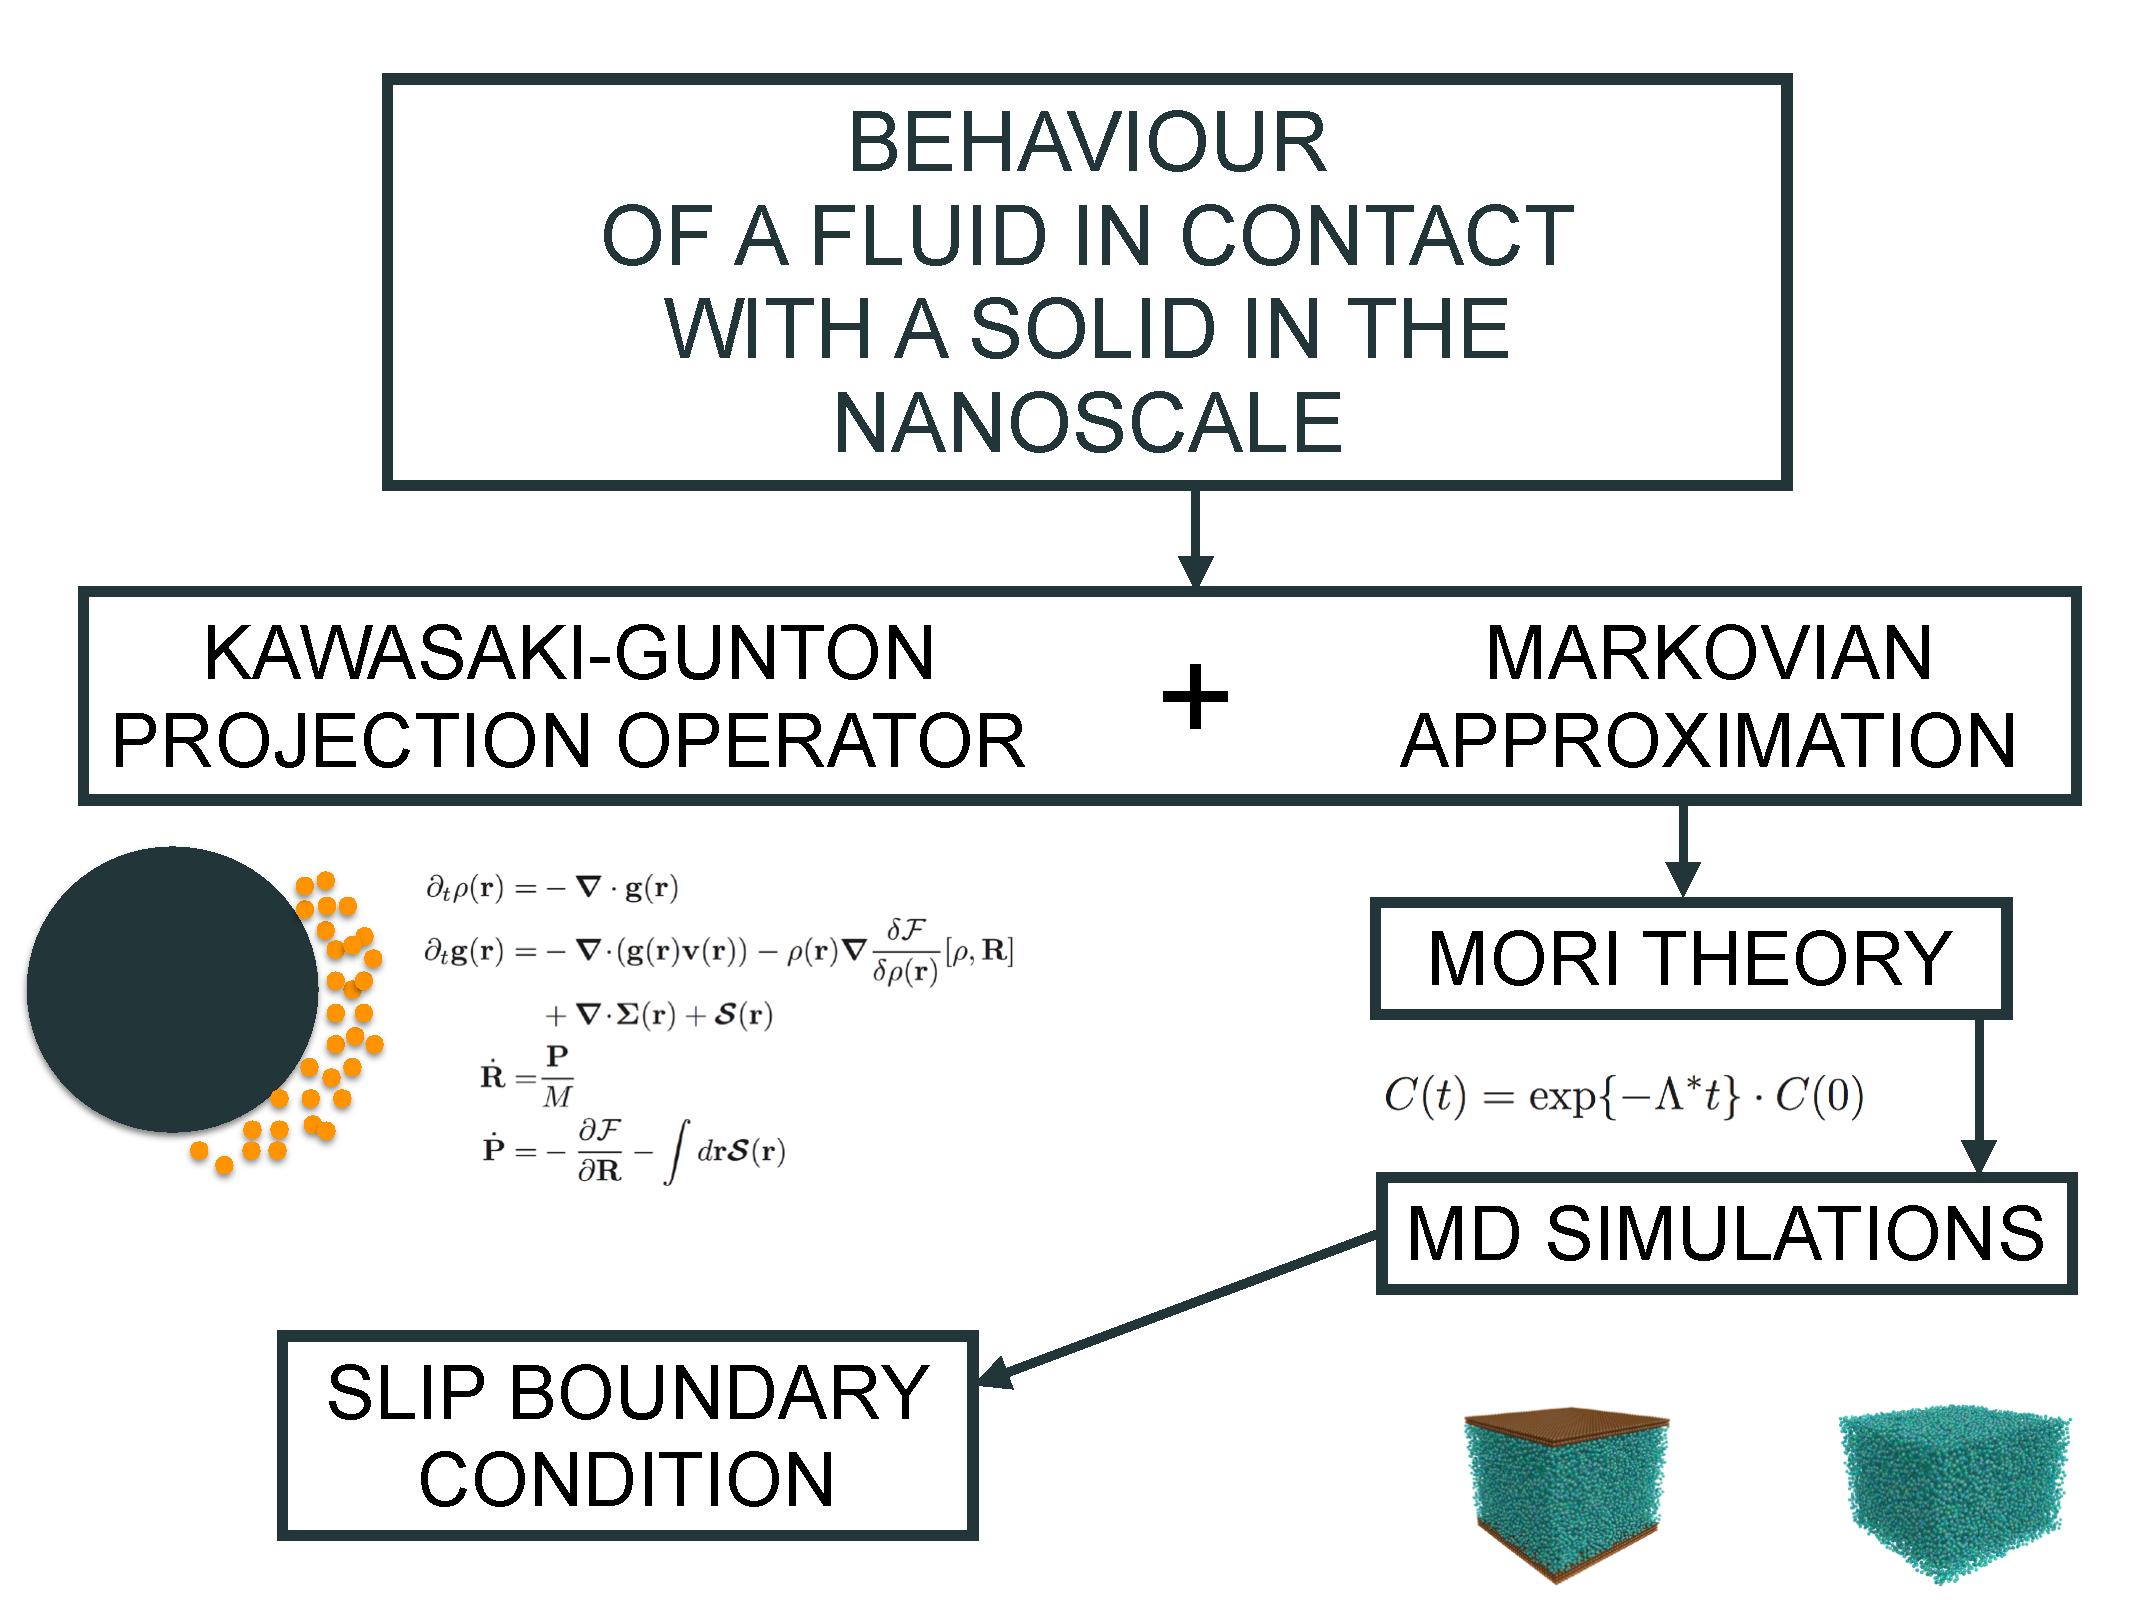
\includegraphics[width=\linewidth]{scheme-thesis}
\end{frame}

\begin{frame}{Roadmap}
  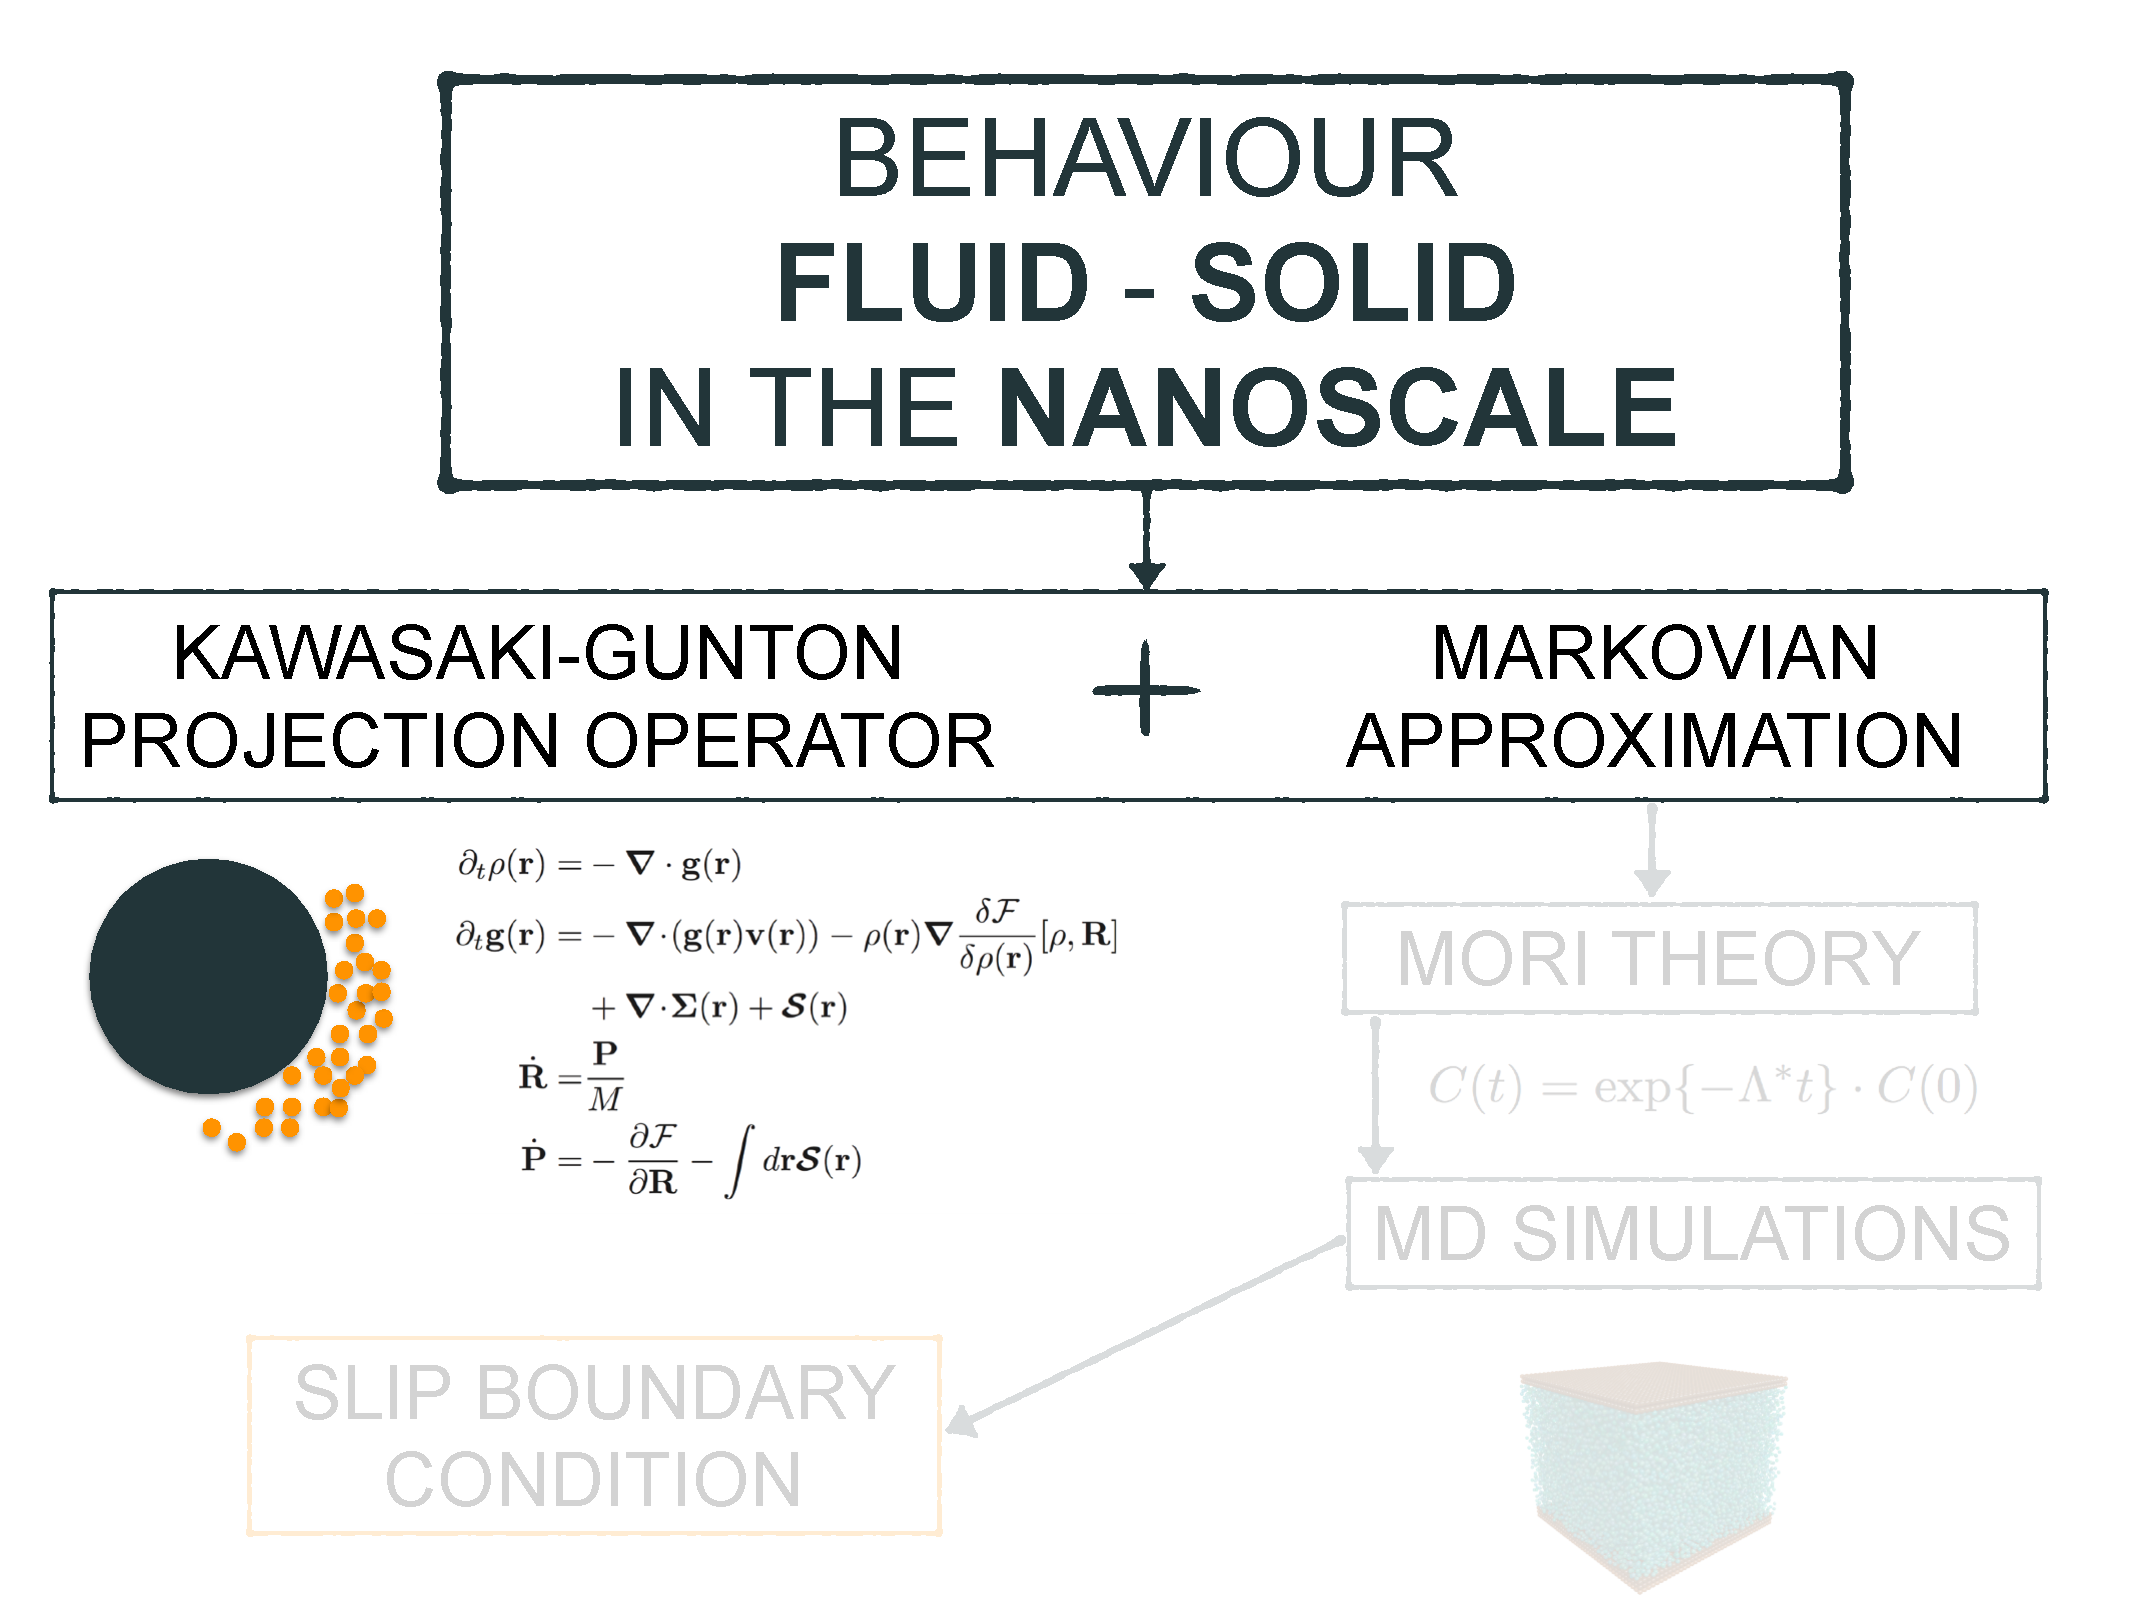
\includegraphics[width=\linewidth]{scheme-thesis-kawasaki}
\end{frame}

\section{Hydrodynamics theory for liquids near solids}
\begin{frame}{The system and the relevant variables}
  \begin{itemize}
    \item<1-> We study a fluid with $N$ particles in contact with a solid sphere of $N'$ particles.
    %\item $z= ({\bf q}_i, {\bf p}_i)$ and $z'= ({\bf q}_{i'}, {\bf p}_{i'})$
    \item<2-> The relevant variables 
      \begin{align}
        \hat{\rho}_{\bf r}(z) &=\sum^{N}_im\delta({\bf r}-{\bf q}_i)
      &&\hat{\bf R}(z)=\frac{1}{N'}\sum_{i'}^{N'}{\bf q}_{i'}
      \nonumber\\
        \hat{\bf g}_{\bf r}(z) &=\sum^{N}_i{\bf p}_i\delta({\bf r}-{\bf q}_i)
      &&\hat{\bf P}(z)=\sum_{i'}^{N'}{\bf p}_{i'}
      \nonumber
      \end{align}
    \item<3-> The derivatives of the relevant variables
      \begin{align}
        i{\cal L} \hat{\rho}_{\bf r}(z) &= -\boldsymbol{\nabla}\esc\hat{\bf g}_{\bf r}(z)
        && i{\cal L}\hat{\bf R}(z) =\frac{\hat{\bf P}(z)}{M}
      \nonumber\\
      i{\cal L}\hat{\bf g}_{\bf r}(z)
          &=-\boldsymbol{\nabla}\cdot \hat{\boldsymbol{\sigma}}_{\bf r}(z)+\hat{{\bf F}}^{\rm s\to l}_{\bf r}(z) 
        &&i{\cal L}\hat{\bf P}(z) =-\int  d{\bf r} \hat{\bf F}^{\rm s\to l}_{\bf r}(z)
         \nonumber
\end{align}
    \end{itemize}
\end{frame}

\begin{frame}{Kawasaki-Gunton projection operator}
  \begin{itemize}
     \item<1-> Separation of timescales between the evolution of the averages of the CG variables, $a_i$, and the decay of the memory kernel 
\begin{equation}
  \frac{\partial}{\partial t}a_i(t) = {\color{blue} v_i(t)} {\color{red} +\sum_j D_{ij}(t) \lambda_j(t)}
\nonumber
\end{equation}
\item<2-> {\color{blue} Reversible term}: $v_i={\rm Tr}[\overline{\rho}_t i{\cal L}\hat{A}_i]$ 
\item<3-> The relevant ensemble: 
  \begin{equation}
  \overline{\rho}(z) = \frac{1}{Z[\lambda]} \rho_0\exp\{-\lambda\!\cdot\!\hat{A}(z)\}
  \nonumber
  \end{equation}
\item<4-> {\color{red} The  dissipative matrix}  is  given  by  the Green-Kubo  formula
\begin{equation}
D_{ij}(t)=\int_0^{\Delta t} dt'\left\langle 
{\cal Q}_t i{\cal L}\hat{A}_j\exp\{i{\cal L}t'\}{\cal Q}_t i{\cal L}\hat{A}_i
\right\rangle^{\lambda(t)}
\label{dij}
\nonumber
\end{equation}
\item<5-> The Kawasaki-Gunton projection operator is given by 
  \begin{align}
    {\cal Q}_{t'}\hat{F}(z) &= \hat{F}(z)- {\rm Tr}[\overline{\rho}_{t'} \hat{F}]
  -\sum_i(\hat{A}_i(z)-a_i(t'))\frac{\partial }{\partial a_i(t')}
  {\rm Tr}[\overline{\rho}_{t'} \hat{F}]
  \label{Q}
  \nonumber
  \end{align}
\end{itemize}
\end{frame}

\begin{frame}{Equations of nanohydrodynamics}
\begin{align}
  \partial_t\rho({\bf r})=&{\color{blue} -\boldsymbol{\nabla}\cdot{\bf g}({\bf r})}
\nonumber\\
\partial_t{\bf g}({\bf r})=&{\color{blue} -\boldsymbol{\nabla}\esc{\left({\bf g}({\bf r}){\bf v}({\bf r})\right)}
-\rho({\bf r})\boldsymbol{\nabla}\frac{\delta {\cal F}}{\delta\rho({\bf r})}[\rho,{\bf R}]}
{\color{red} +\boldsymbol{\nabla}\esc\boldsymbol{\Sigma}({\bf r})+\boldsymbol{{\cal S}}({\bf r})}
\nonumber\\
\dot{\bf R}=&{\color{blue} \frac{\bf P}{M}}
\nonumber\\
\dot{\bf P}=&{\color{blue} -\frac{\partial {\cal F}}{\partial {\bf R}}}
{\color{red} -\int d {{\bf r}}\boldsymbol{{\cal S}}({\bf r})}
\nonumber
\end{align}

\begin{itemize}
  \item ${\cal F}[\rho, {\bf R}]$: free energy density functional of a fluid in the presence of a solid sphere.
  \item $\Sigma({\bf r})$: fluid stress tensor.
  \item ${\cal S}({\bf r})$: irreversible surface force density on the fluid.
\end{itemize}
\end{frame}

\begin{frame}{The fluid stress tensor and the irreversible force}
  \begin{itemize}
    \item<1-> The fluid stress tensor ${\color{red} \Sigma({\bf r})}$ is given by 
  \begin{align}
  \boldsymbol{\Sigma}^{\alpha\beta}({\bf r})&=
\int d{\bf r}'
\boldsymbol{\eta}^{\alpha\beta\alpha'\beta'}_{{\bf r}{\bf r}'}
\boldsymbol{\nabla}_{{\bf r}'}^{\beta'}{\bf v}^{\alpha'}({\bf r}')
\nonumber
\end{align}
\item<2-> The irreversible surface force density on the fluid ${\color{red} {\cal S}({\bf r})}$
\begin{align}
  \boldsymbol{{\cal S}}^\alpha({\bf r})=&
-\int d{\bf r}'{\bf G}^{\alpha\alpha'\beta'}_{{\bf r}{\bf r}'}
\boldsymbol{\nabla}_{{\bf r}'}^{\beta'} {\bf v}^{\alpha'}({\bf r}')
+\boldsymbol{\nabla}_{{\bf r}}^{\beta}\int d{\bf r}'{\bf H}^{\alpha\beta\alpha'}_{{\bf r}{\bf r}'}
( {\bf v}^{\alpha'}({\bf r}')-{\bf V}^{\alpha'})
\nonumber\\
&-\int d{\bf r}'
\boldsymbol{\gamma}^{\alpha\alpha'}_{{\bf r}{\bf r}'}( {\bf v}^{\alpha'}({\bf r}')
-{\bf V}^{\alpha'})
\nonumber
\end{align}
\end{itemize}
\end{frame}

\begin{frame}{The transport kernels}
\begin{align}
  \boldsymbol{\eta}_{{\bf  r}{\bf r}'} &\equiv
\frac{1}{k_BT}\int_0^{\Delta t} dt'\langle 
{\cal Q}_t\hat{\boldsymbol{\sigma}}_{{\bf r}}(t')
{\cal Q}_t\hat{\boldsymbol{\sigma}}_{{\bf r}'}\rangle^{\lambda(t)}
\nonumber \\
{\bf H}_{{\bf r}{\bf r}'}&\equiv\frac{1}{k_BT}\int_0^{\Delta t} dt'
\langle {\cal Q}_t\hat{\boldsymbol{\sigma}}_{{\bf r}}(t')
{\cal Q}_t\hat{\bf F}^{\rm s\to l}_{{\bf r}'}\rangle^{\lambda(t)}
\nonumber\\
{\bf G}_{{\bf r}{\bf r}'}&\equiv\frac{1}{k_BT}\int_0^{\Delta t} dt'
\langle {\cal Q}_t\hat{\bf F}^{\rm s\to l}_{{\bf r}}(t')
{\cal Q}_t\hat{\boldsymbol{\sigma}}_{{\bf r}'}\rangle^{\lambda(t)}
\nonumber\\
\boldsymbol{\gamma}_{{\bf  r}{\bf r}'}&\equiv\frac{1}{k_BT}\int_0^{\Delta t} dt'
\langle 
{\cal Q}_t\hat{\bf F}^{\rm s\to l}_{{\bf r}}(t')
{\cal Q}_t\hat{\bf F}^{\rm s\to l}_{{\bf r}'}\rangle^{\lambda(t)}
\nonumber
\end{align}
\end{frame}


\begin{frame}{Discrete basis function I}
  %\begin{itemize}
    %\item 
  $N_{\rm bin}$ bins with dimensions $L_x$, $L_y$, $\Delta z$. ($\Delta z = \frac{L_z}{N_{\rm bin}}$). 
      \begin{center}
        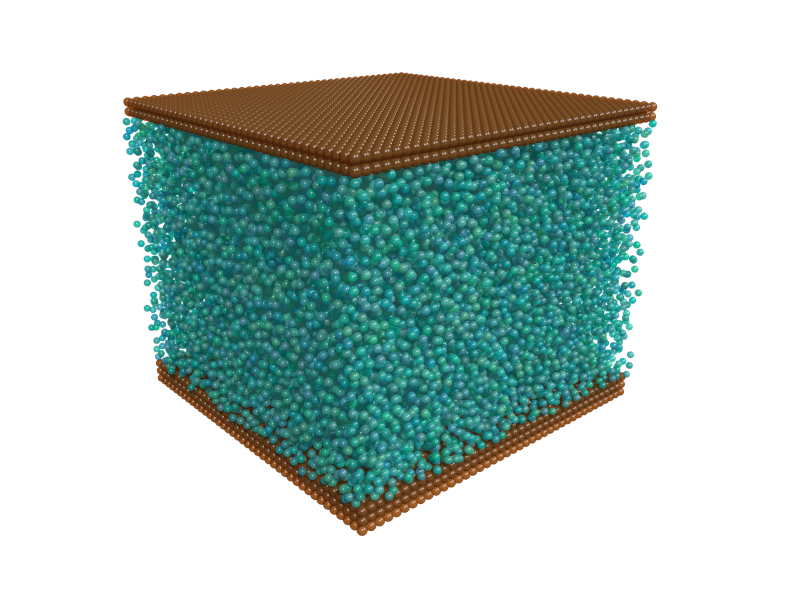
\includegraphics[width=.5\linewidth]{PRL3_gold2_wo_layers_wo_diffuse}
        %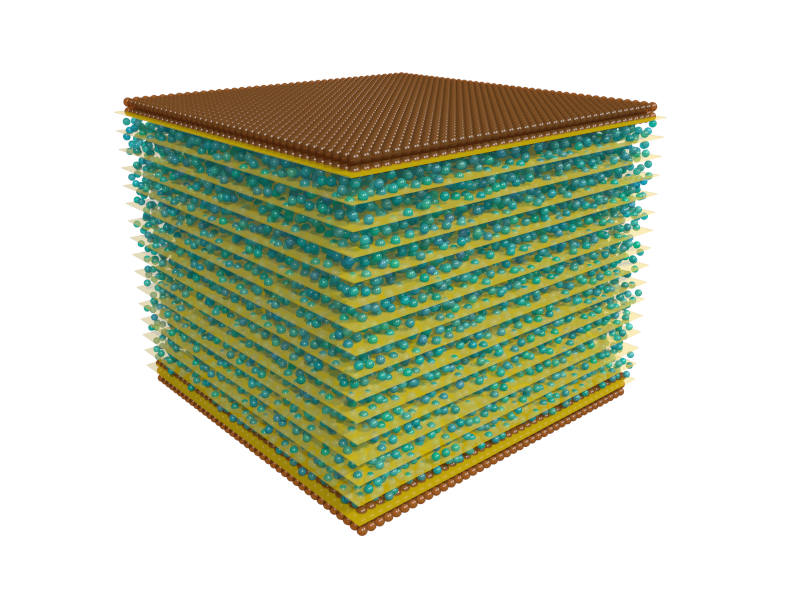
\includegraphics[width=.5\linewidth]{PRL3_gold2_wo_diffuse}
        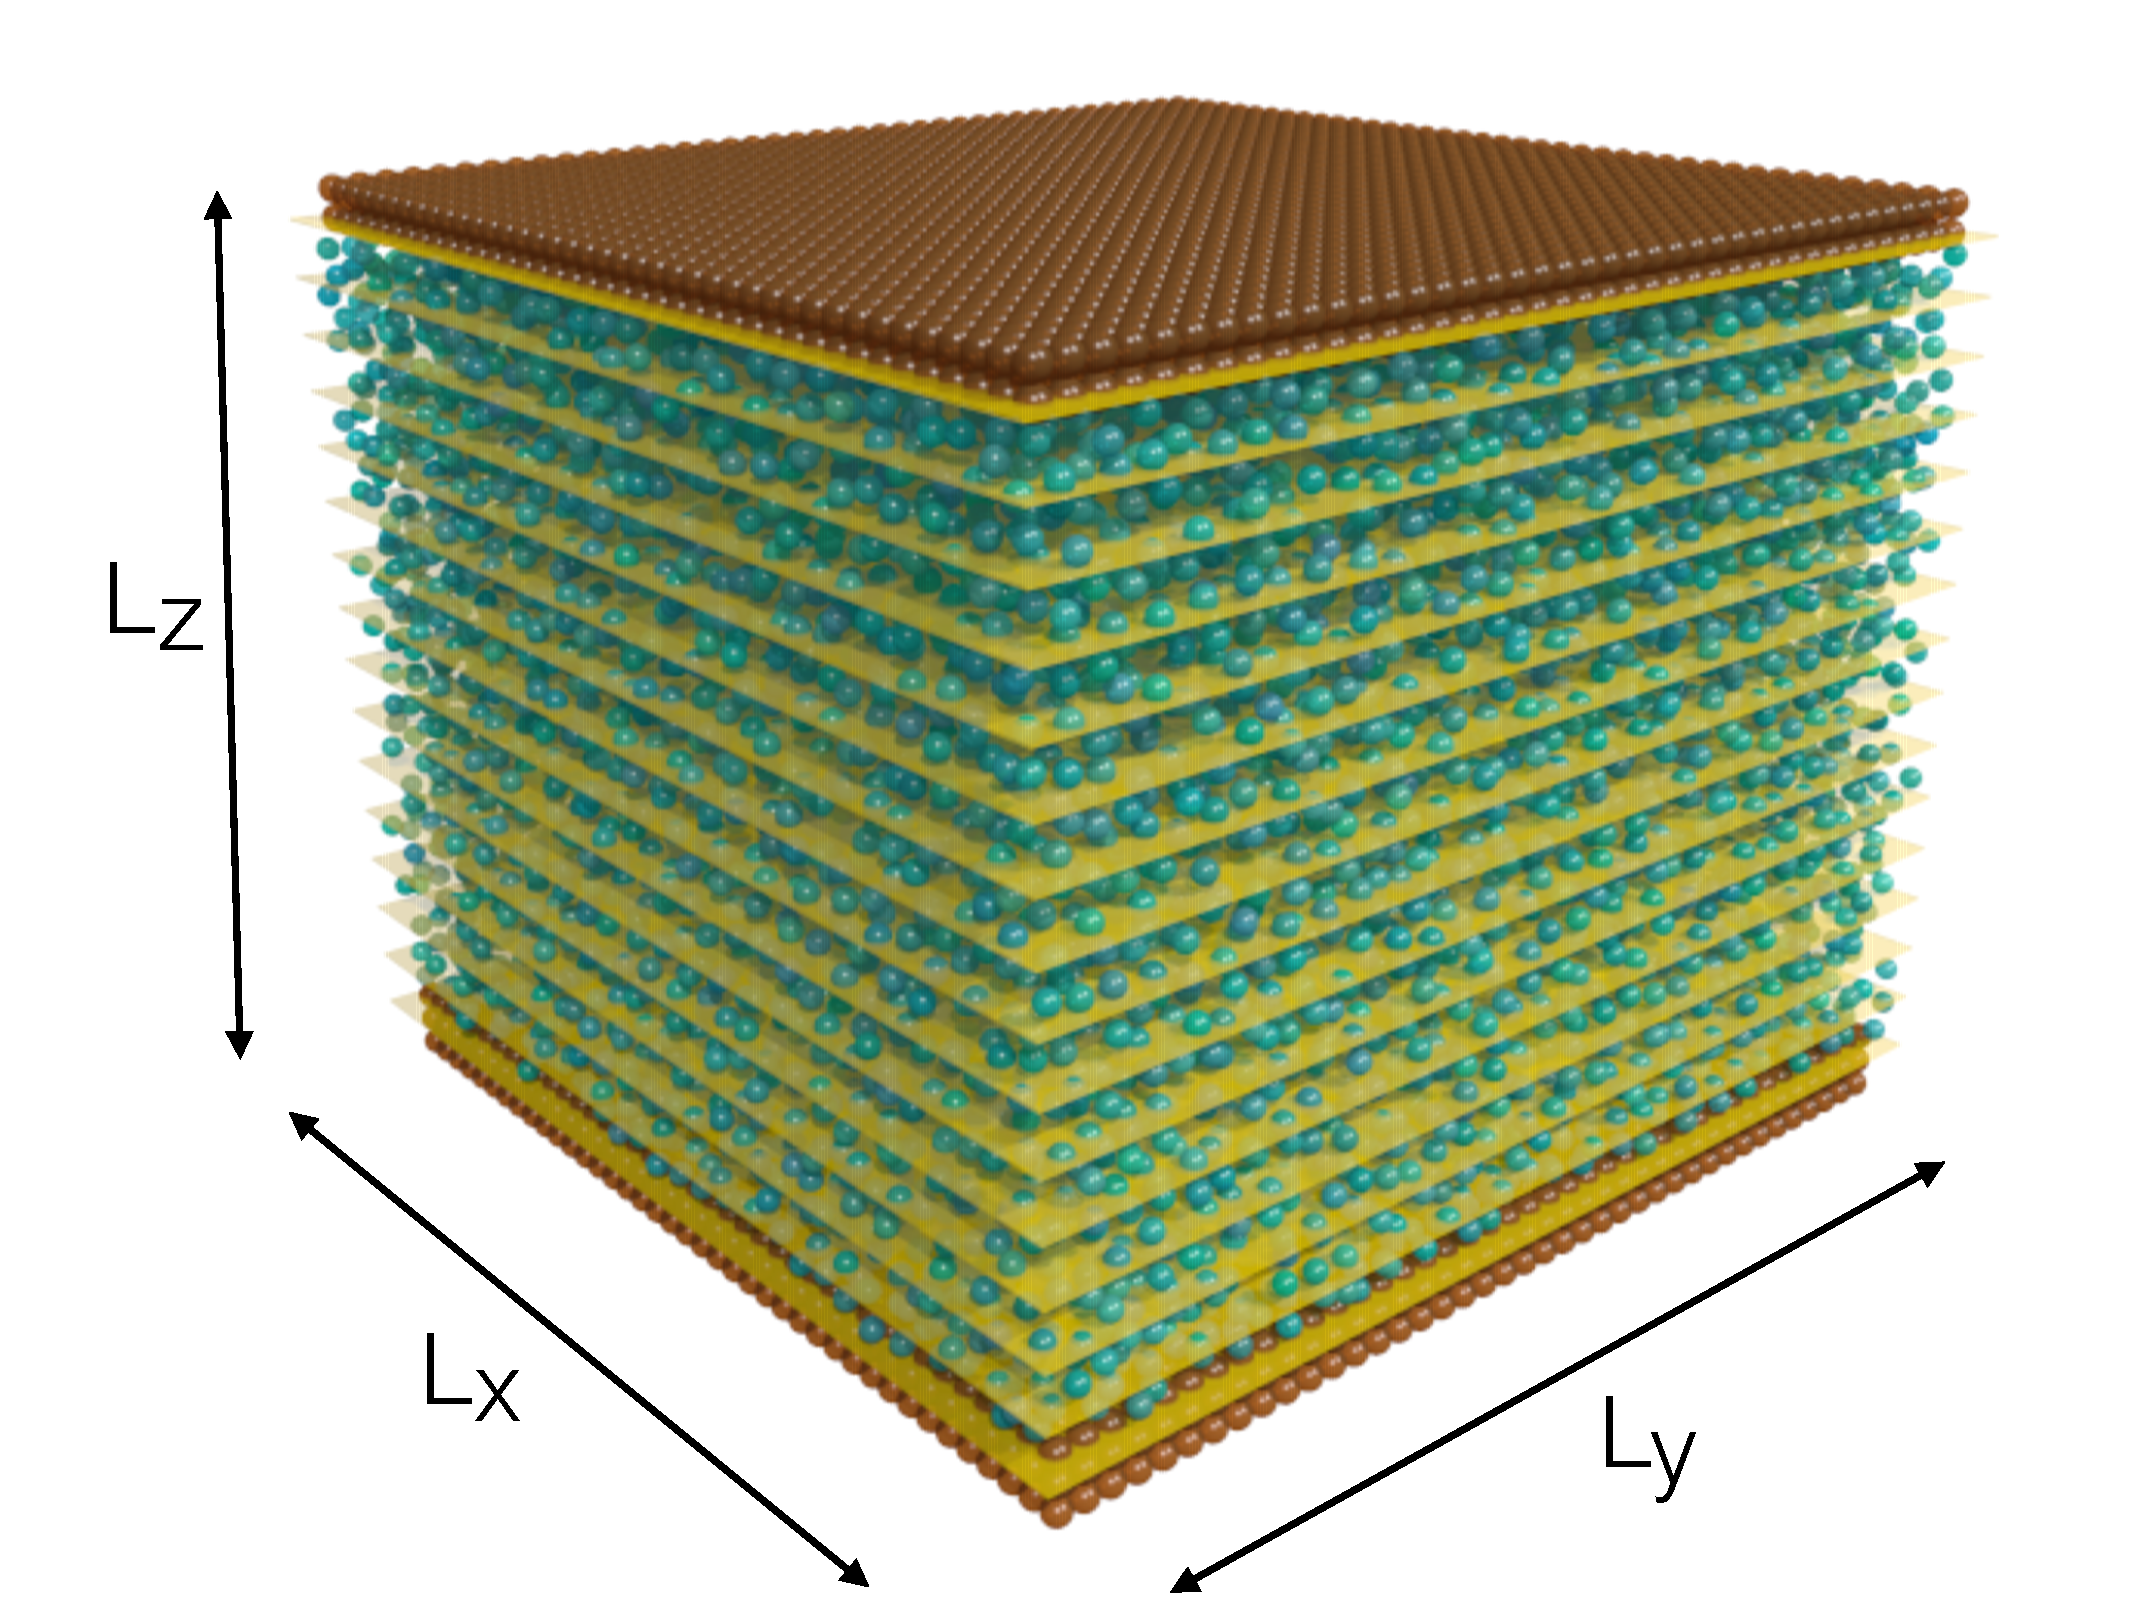
\includegraphics[width=.45\linewidth]{scheme-bines}
      \end{center}
  \end{frame}
\begin{frame}{Discrete basis function II}
    %\item  
  Characteristic function $\chi_{\mu}({\bf r})$ and finite element linear basis function $\Phi_{\mu}({\bf r})$
    \begin{align}
    \chi_\mu({\bf r})&=\theta(z_{\mu+ 1}-z)\theta(z-z_\mu)=\chi_\mu(z)
    \nonumber
    \end{align}
    \begin{align}
      \Phi_\mu({\bf r})=\chi_\mu(z)\frac{z_{\mu+1}-z}{\Delta z}+\chi_{\mu-1}(z)\frac{z-z_{\mu-1}}{\Delta z}
      \nonumber
    \end{align}
    \begin{center} 
      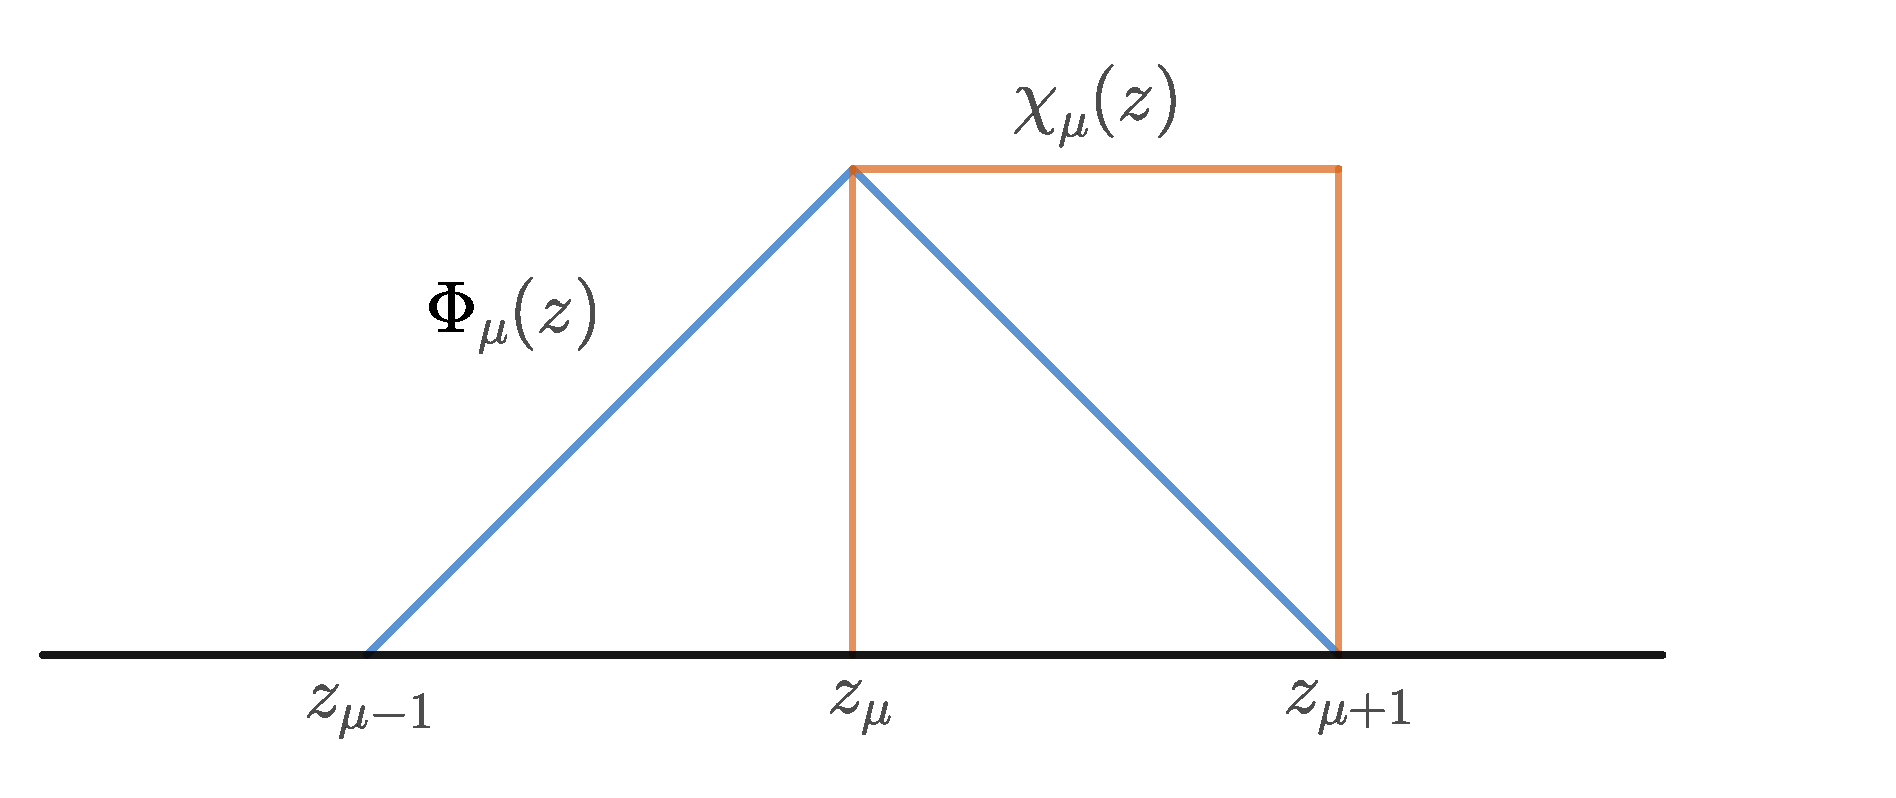
\includegraphics[width = \linewidth]{psichi}
      %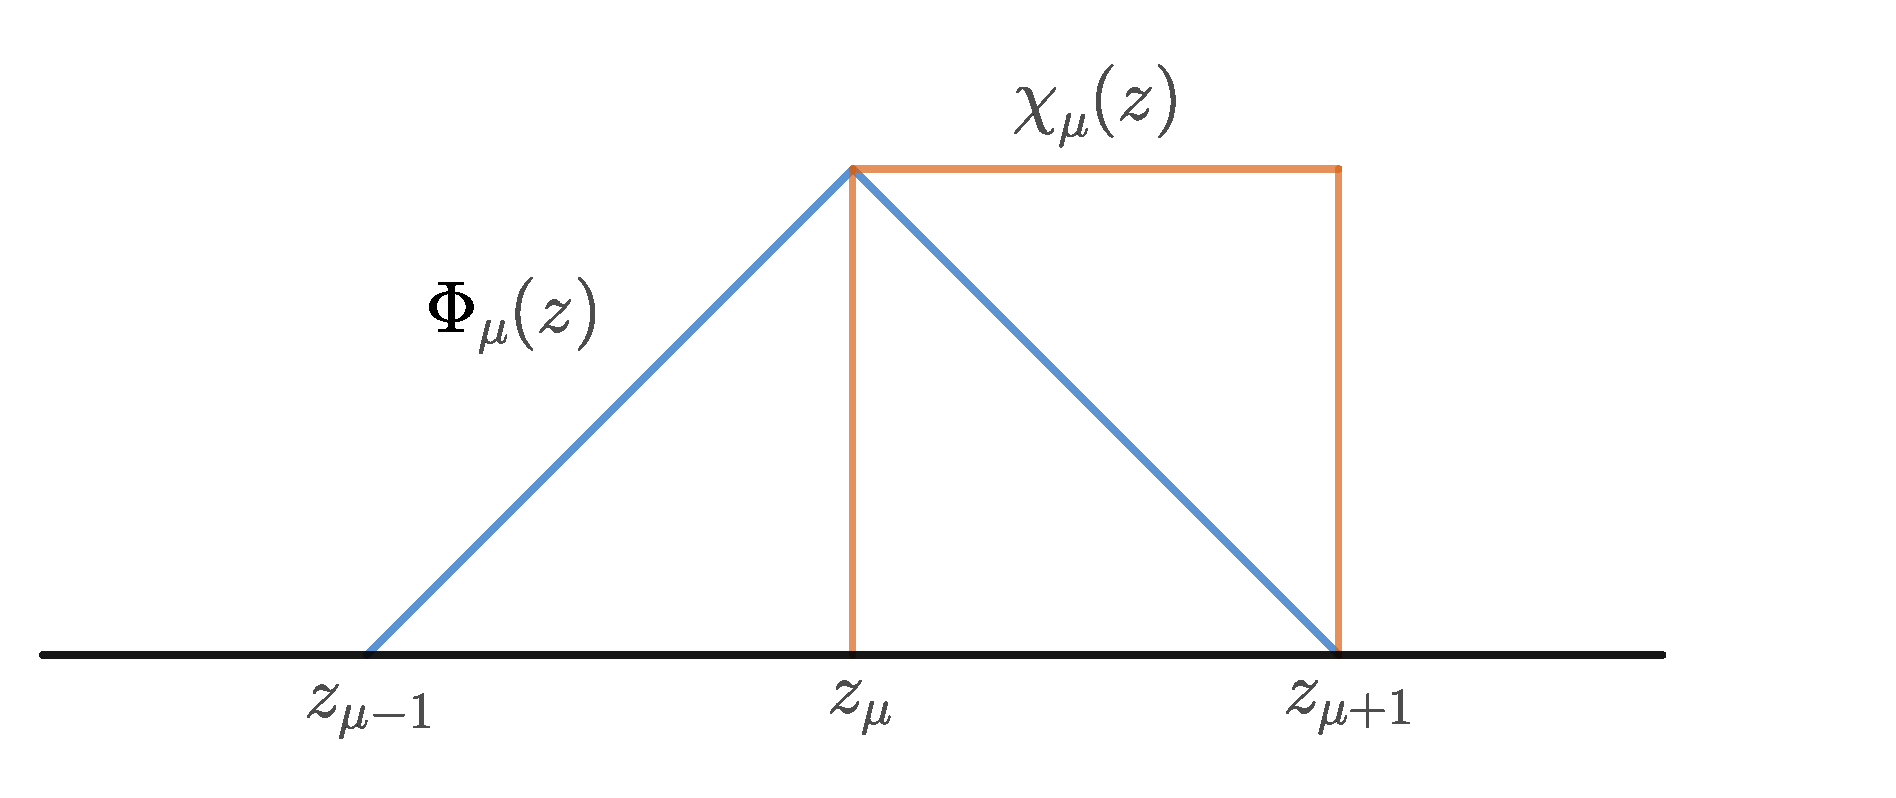
\includegraphics[scale=0.16]{psichi}
    \end{center}
  %\end{itemize}
\end{frame}

%\begin{frame}{Dual basis functions and mass matrix}
%  \begin{itemize}
%  \item We can contruct continuum and discrete fields from dual basis functions $\delta_{\mu}({\bf r})$ and $\psi_\mu({\bf r})$ 
%    \begin{align}
%      v_\mu=\int d{\bf r}v({\bf r})\delta_\mu({\bf r}),&&
%        \overline{v}({\bf r}) =\sum_{\mu}v_\mu\psi_\mu({\bf r})
%    \nonumber
%    \end{align}
%    \item The usual mass matrix of the finite element method is
%      \begin{align}
%      M^\Phi_{\mu\nu}&=\llg\Phi_\mu\Phi_\nu\rlg  
%      \nonumber
%      \end{align}
%      where we have introduce the notation $\llg\cdots\rlg=\int d{\bf r}...$
%    \item We introduce the discrete velocity field in terms of $M^\Phi_{\mu\nu}$
%      \begin{align}
%        \tilde{{\bf v}}_{\mu}=\sum_{\nu}{\cal V}_{\mu}[M^{\Phi}]^{-1}_{\mu\nu}{\bf v}_{\nu}
%        \nonumber
%      \end{align}
%  \end{itemize}
%\end{frame}

\begin{frame}{Discrete equations of nanohydrodynamics}
\begin{align}
  %\frac{d}{dt}\rho_\mu&=  {\color{blue} \llg\overline{\rho} \; \overline{\bf v}\boldsymbol{\nabla}\delta_\mu \rlg}
  \frac{d}{dt}\rho_\mu&=  {\color{blue} \int d{\bf r}\overline{\rho} \; \overline{\bf v}\boldsymbol{\nabla}\delta_\mu }
\nonumber\\
\frac{d}{dt}{\bf g}_\mu&=
%{\color{blue} \llg\overline{\rho} \overline{\bf v}\;\overline{\bf v}\esc\boldsymbol{\nabla}\delta_{\mu}\rlg
  {\color{blue} \int d{\bf r}\overline{\rho} \overline{\bf v}\;\overline{\bf v}\esc\boldsymbol{\nabla}\delta_{\mu}
%-\sum_\nu\llg\overline{\rho}\delta_{\mu}\boldsymbol{\nabla}\delta_{\nu}\rlg
%\frac{\partial  F}{\partial \rho_{\nu}}(\rho)}
  -\sum_\nu\int d{\bf r}\overline{\rho}\delta_{\mu}\boldsymbol{\nabla}\delta_{\nu}
\frac{\partial  F}{\partial \rho_{\nu}}(\rho)}
\nonumber\\
&{\color{red}-\sum_{\nu}{\cal V}_\nu \frac{{\bf n}\esc\left[\boldsymbol{\eta}_{\mu\nu}-\boldsymbol{\eta}_{\mu-1\nu}-\boldsymbol{\eta}_{\mu\nu-1}+\boldsymbol{\eta}_{\mu-1\nu-1}\right]}{\Delta z^2}:{\bf n}\tilde{\bf v}_\nu}
\nonumber\\
&{\color{red}+\sum_{\nu}{\cal V}_\nu\frac{\left[{\bf G}_{\mu\nu}-{\bf G}_{\mu\nu-1}\right]}{\Delta z}\esc{\bf n}\tilde{\bf v}_\nu}
\nonumber\\
&{\color{red}+\sum_{\nu}{\cal V}_\nu\frac{{\bf n}\esc\left[{\bf H}_{\mu\nu}-{\bf H}_{\mu-1\nu}\right]}{\Delta z}\esc\tilde{\bf v}_\nu}
\nonumber\\
&{\color{red}-\sum_{\nu}{\cal V}_\nu\boldsymbol{\gamma}_{\mu\nu}\esc\tilde{\bf v}_\nu}
\nonumber
\end{align}
\end{frame}

\begin{frame}{Simpler theory}
  \begin{itemize}
    \item<1-> The amount of information to compute the hydrodynamic equations is exceedingly large:
      \begin{itemize}
        \item $\boldsymbol{\eta}$ has 36 independent components. 
        \item ${\bf G}$ and ${\bf H}$ have 21 independent components. 
        \item $\boldsymbol{\gamma}$ has 9 independent components. 
      \end{itemize}
    \item<2-> Two simplifications
      \begin{enumerate}
    \item The interactions felt by the fluid due to the walls are statistically planar and isotropic (planar walls).
    \item Planar flows: the hydrodynamic flow depends only on the coordinate perpendicular to the walls. 
      \end{enumerate}
    \item<3-> Under the simplification we may separate the evolution of the selected variables in two contribution: normal and tangent.
    %\item<3-> In order to compare the hydrodynamic equations with the MD simulations we need a discrete version of the theory. 
    \end{itemize}
\end{frame}

%\begin{frame}{Normal and tangent evolution}
%\begin{itemize}
%  \item The normal evolution 
%\begin{align}
%  \frac{d}{dt}\rho_\mu=&  {\color{blue} \llg\overline{\rho} \; \overline{v}^{z}{\nabla}^{z}\delta_\mu \rlg}
%\nonumber\\
%    \frac{d}{dt}{{\bf g}}^{z}_\mu=&
%{\color{blue} \llg\overline{\rho}\; \overline{v}^{z}\;\overline{v}^{z}{\nabla}^{z}\delta_{\mu}\rlg
%-\llg\overline{\rho}\delta_{\mu}{\nabla}^{z}\delta_{\nu}\rlg
%\frac{\partial  F}{\partial \rho_{\nu}}(\rho)}
%{\color{red} +M_{\mu\nu}^{\bot}{\cal V}_\nu\tilde{v}^{z}_\nu}
%\nonumber
%\end{align}
%  \item The parallel evolution for $\alpha=x,y$  
%\begin{align}
%  \frac{d}{dt}{{\bf g}}^\alpha_\mu=&{\color{red}-M_{\mu\nu}^{||}{\cal V}_\nu\tilde{v}^\alpha_\nu}
%\nonumber
%\end{align}
%\item The dissipative matrix for $\odot=||,\bot$
%\begin{align}
%M^{\odot}_{\mu\nu} 
%=&-\frac{\eta^{\odot}_{\mu\nu}-\eta^{\odot}_{\mu-1\nu}-\eta^{\odot}_{\mu\nu-1}+\eta^{\odot}_{\mu-1\nu-1}}{\Delta z^2}
%+\frac{{G}^{\odot}_{\mu\nu}-{G}^{\odot}_{\mu\nu-1}}{\Delta z} \nonumber \\
%&+\frac{{H}^{\odot}_{\mu\nu}-{H}^{\odot}_{\mu-1\nu}}{\Delta z}
%-{\gamma}^{\odot}_{\mu\nu}
%\nonumber
%\end{align}
%\end{itemize}
%\end{frame}

\begin{frame}{The discrete transport kernels}
\begin{align}
\eta^{||}_{\mu\nu}&
=\frac{1}{k_BT}\int_0^\tau  dt\left\langle 
{\cal Q}\hat{\boldsymbol{\sigma}}^{xz}_\mu(t){\cal Q}\hat{\boldsymbol{\sigma}}^{xz}_\nu
\right\rangle&&
%\nonumber\\
\eta^{\bot}_{\mu\nu}
= \frac{1}{k_BT}\int_0^\tau  dt\langle 
{\cal Q}\hat{\boldsymbol{\sigma}}^{zz}_\mu(t)
{\cal Q}\hat{\boldsymbol{\sigma}}^{zz}_\nu\rangle
\nonumber\\
G^{||}_{\mu\nu}&
=\frac{1}{k_BT} \int_0^\tau  dt
\left\langle{\cal Q}\hat{\bf F}^{x}_\mu(t)
{\cal Q}\hat{\boldsymbol{\sigma}}^{xz}_\nu
\right\rangle&&
%\nonumber\\
G^{\bot}_{\mu\nu}=\frac{1}{k_BT} \int_0^\tau  dt
\left\langle {\cal Q}\hat{\bf F}^{z}_\mu(t)
{\cal Q}\hat{\boldsymbol{\sigma}}^{zz}_\nu
\right\rangle
\nonumber\\
H^{||}_{\mu\nu}&
=\frac{1}{k_BT} 
\int_0^\tau  dt
\left\langle{\cal Q}\hat{\boldsymbol{\sigma}}^{xz}_\mu(t){\cal Q}\hat{\bf F}^{x}_\nu\right\rangle&&
%\nonumber\\
H^\bot_{\mu\nu}=\frac{1}{k_BT} 
\int_0^\tau  dt\left\langle {\cal Q}\hat{\boldsymbol{\sigma}}^{zz}_\mu(t){\cal Q}\hat{\bf F}^{z}_\nu\right\rangle
\nonumber\\
\gamma^{||}_{\mu\nu}&=
\frac{1}{k_BT} \int_0^\tau  dt
\left\langle 
{\cal Q}\hat{\bf F}^{x}_\mu(t)
{\cal Q}\hat{\bf F}^{x}_\nu\right\rangle&&
%\nonumber\\
\gamma^{\bot}_{\mu\nu}=
\frac{1}{k_BT} \int_0^\tau  dt\left\langle 
{\cal Q}\hat{\bf F}^{z}_\mu(t){\cal Q}\hat{\bf F}^{z}_\nu
\right\rangle
\nonumber
\end{align}
\end{frame}

\begin{frame}{Roadmap}
  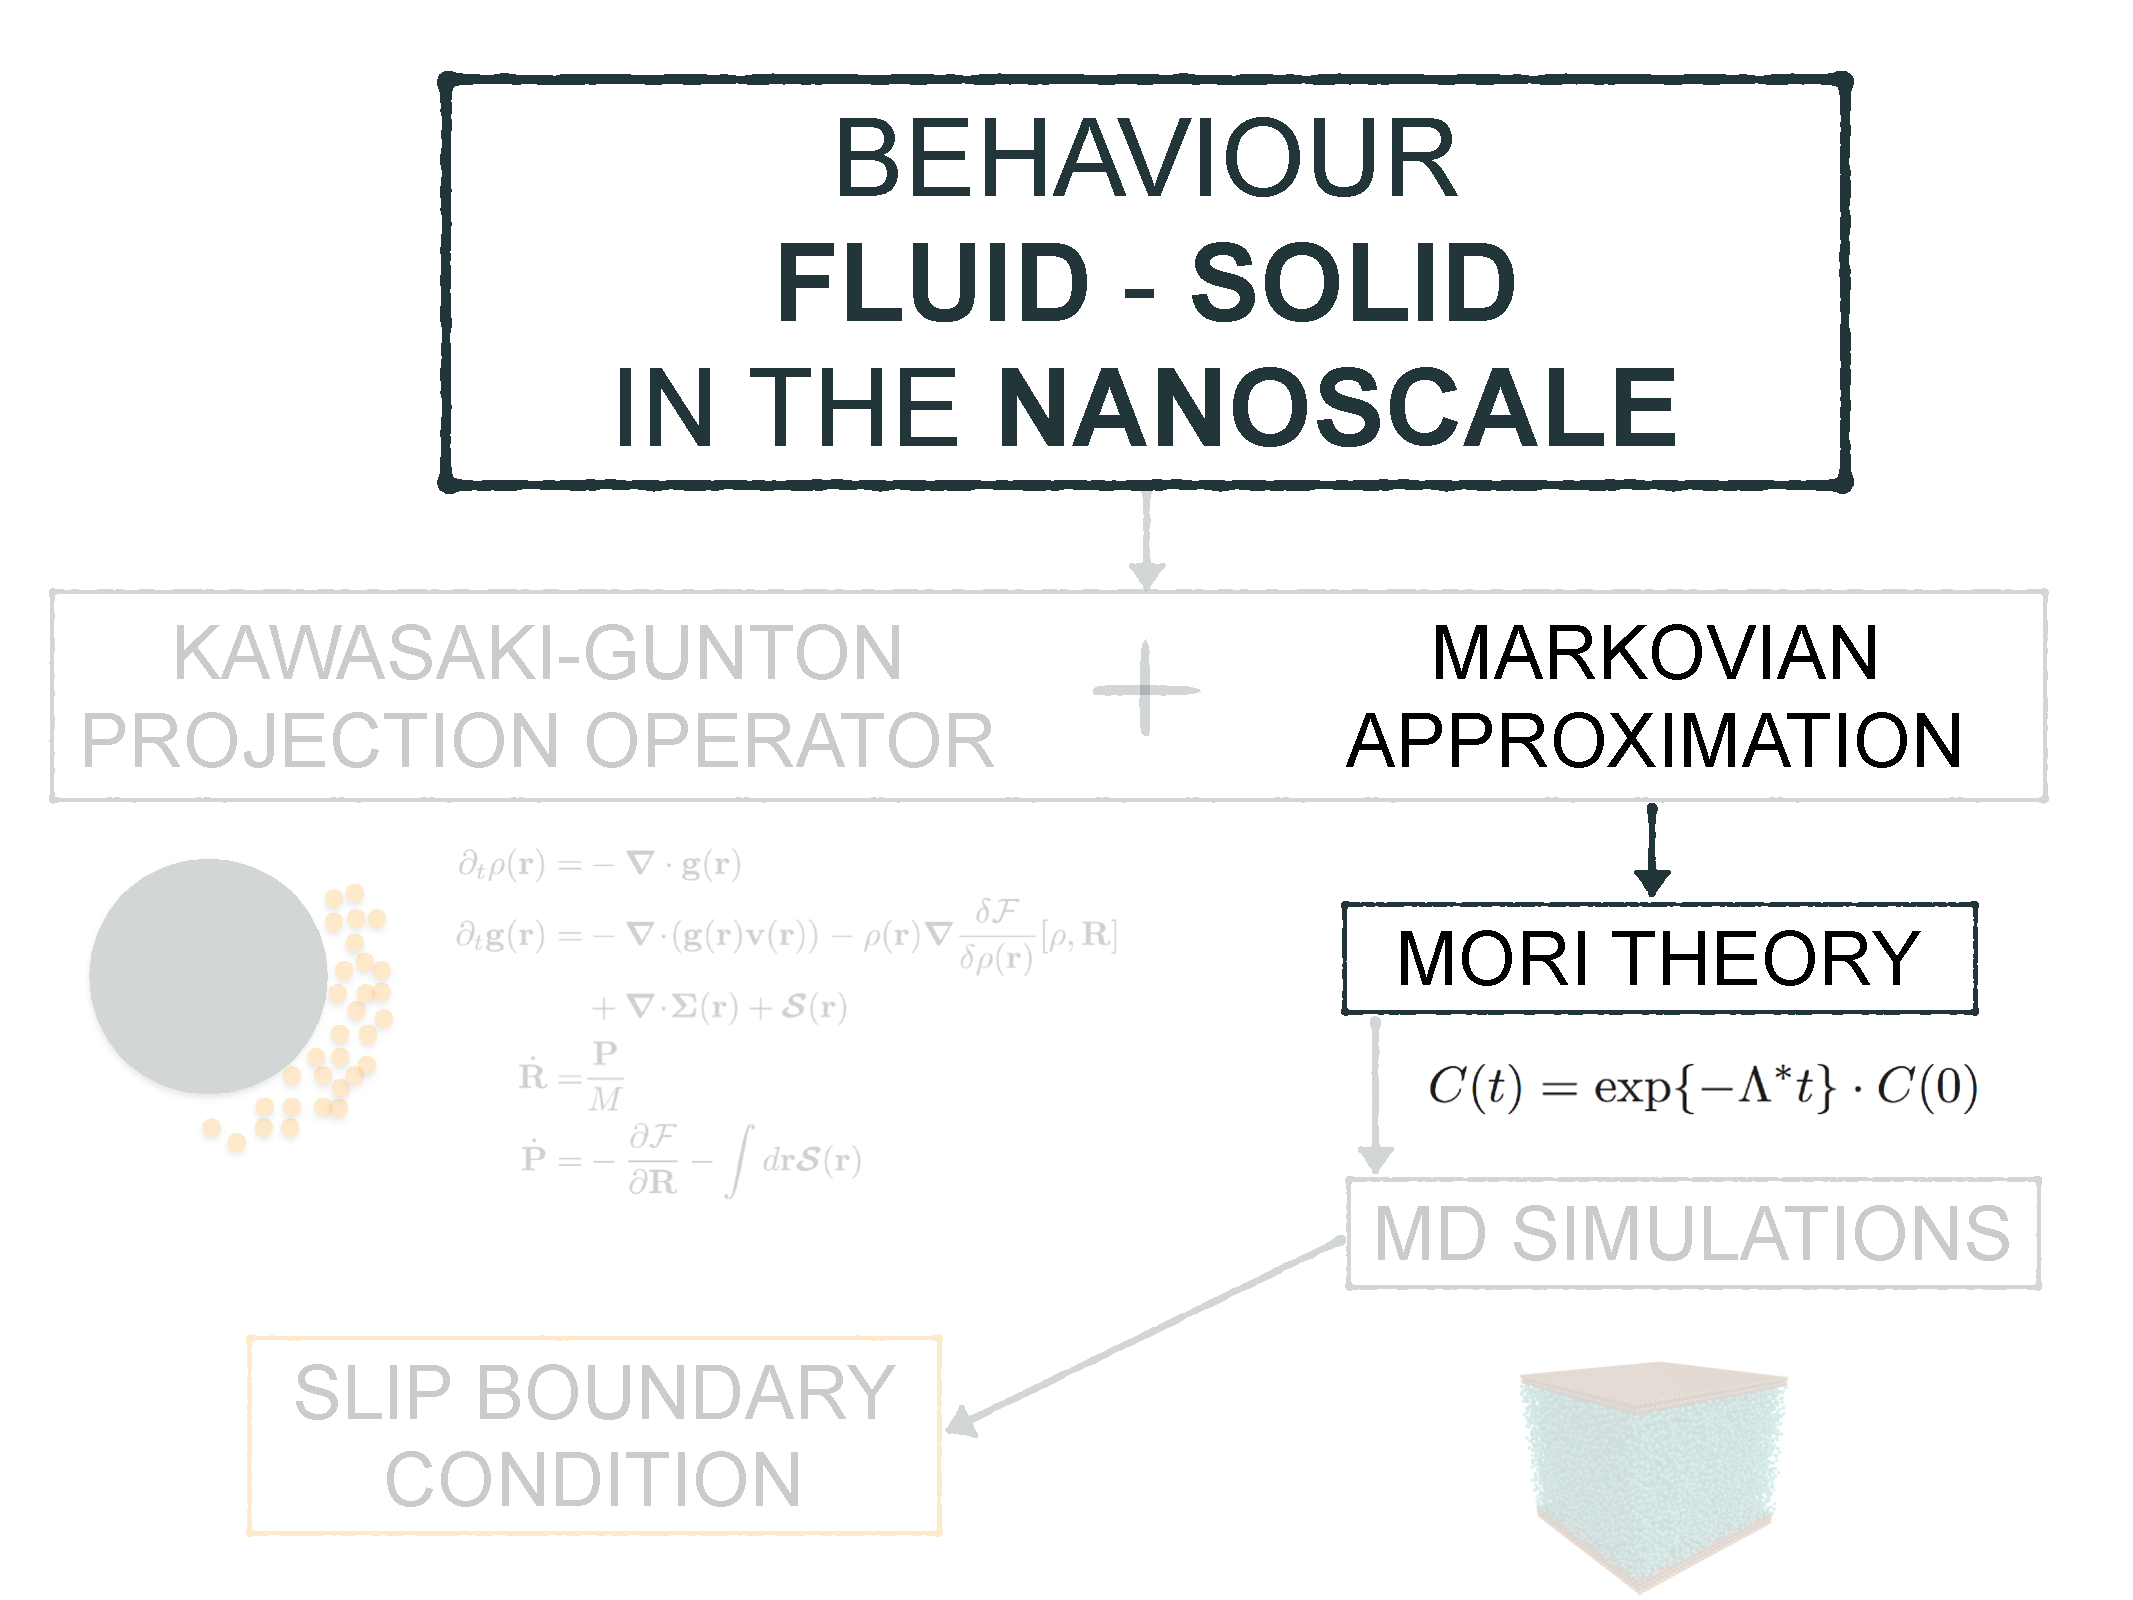
\includegraphics[width=\linewidth]{scheme-thesis-markovian}
\end{frame}

\section{Space and time locality for unconfined fluids}
\begin{frame}{Mori's theory}
  \begin{itemize}
    \item<1-> Linear dynamic equations for the correlations of $\hat{A}(t)$
\begin{align}
  \frac{d}{dt}C(t)&=-L\esc C^{-1}(0)\esc C(t)
  -{\color{red}\int_0^tdt' \Gamma(t-t')\esc C^{-1}(0)\esc  C(t')}
\nonumber
\end{align}
where  $L=\langle \hat{A}i{\cal L}\hat{A}^T\rangle$.
%where the following matrices have been introduced
%\begin{align}
%  L&=\langle \hat{A}i{\cal L}\hat{A}^T\rangle \nonumber \\
%  C(0)&=\langle \hat{A}\hat{A}^T\rangle \nonumber \\
%\Gamma(t)&=\langle F^+(t)F^{+T}(0)\rangle
%\nonumber
%\end{align}
%\item<2-> The projected forces are given by
%\begin{align}
%F^+(t)&= \exp\{{\cal Q}i{\cal L}t\} {\cal Q}i{\cal L}\hat{A}  
%\nonumber
%\end{align}
%\item<3-> ${\cal Q}=1-{\cal P}$ where  ${\cal P}$  is Mori's  projector 
%\begin{align}
%  {\cal P}\hat{F}(z) = \langle \hat{F}\rangle+ \langle \hat{F}\hat{A}^T \rangle\esc  C^{-1}(0)\esc  \hat{A}(z)
%\nonumber
%\end{align}
%\end{itemize}
%\end{frame}

%\begin{frame}{Markovian approximation}
%  \begin{itemize}
    %\item Memory-less term 
    \item Markovian approximation
  \begin{align}
{\color{red}\int_0^tdt' \Gamma(t-t')\esc C^{-1}(0)\esc  C(t')} \simeq M^* C^{-1}(0)C(t)
\nonumber
\end{align}
\item Mori's equation and Markovian approximation
\begin{align}
  \frac{d}{dt}C(t) &= - (L+M^*)\esc C^{-1}(0)\esc C(t) 
                     \equiv \Lambda^*\esc C(t)
  \nonumber
\end{align}
%\item For a linear Markovian theory the only possibility for a correlation is to decay in an exponential matrix way
\item Exponential matrix decay 
\begin{align}
  C(t)=\exp\{-\Lambda^* (t-\tau)\}\esc C(\tau)
\nonumber
\end{align}
\item {\bf We need to find a constant matrix $\boldsymbol{\Lambda^*}$}.
\end{itemize}
\end{frame}

\begin{frame}{Unconfined fluid. Simulation set up}
  \begin{center}
  %\begin{itemize}
  %\item The system
  \begin{figure}
    %\includegraphics[width=0.5\linewidth]{temp_wo_walls}
    %\includegraphics[width=0.5\linewidth]{temp_wo_walls}
    \includegraphics[width=0.5\linewidth]{sim-pbc-box}
%    \includegraphics[width=0.5\linewidth]{temp_wo_walls_w_layers2}
\end{figure}
%\item The relevant variable
%\begin{align}
%  \hat{\bf g}_\mu(z)= \sum_i^N{\bf p}_i\delta_\mu({\bf r}_i)
%%  i{\cal L}  \hat{g}_{\mu}(z)=-\frac{\hat{\sigma}^{xz}_{\mu}-\hat{\sigma}^{xz}_{\mu-1}}{\Delta z}
%\nonumber
%\end{align}
%\end{itemize}
    \begin{itemize}
     \item<1-> $L_{x}=40$, $L_{y}=40$, $L_{z}=30$.
     \item<2-> $28749$ particles.
     \item<3-> LJ potential truncated at $\sigma=2.5$.
     \item<4-> $dt=2\cdot 10^{-3}$ in reduced units. 
    \end{itemize}
  \end{center}
\end{frame}


\begin{frame}{Unconfined fluid. Simulation set up}
  \begin{figure}
    \includegraphics[width=0.5\linewidth]{sim-pbc-box-bin}
  \end{figure}
   \begin{itemize}
     %\item Simulation of $28749$ particles interacting with a LJ potential truncated at $\sigma=2.5$.
     %\item Box size $40x40x30$.
     \item<1-> Equilibration stage
       \begin{itemize}
         \item Langevin thermostat for $10^5$ timesteps: $T=2.0$, $\rho=0.6$.
         \item NVE microcanonical conditions for a further $10^5$ timesteps.
          \end{itemize}
        \item<2-> Production stage
       \begin{itemize}
         \item $1.5\times10^6$ timesteps.
         \item $z$ axis binned in $60$ bins $\mu$. {$\boldsymbol{\Delta} {\bf z=0.5}\boldsymbol{\sigma}$}.
         \item $g_{\mu}^x(t)$ recorded every $10$ timesteps.
         \end{itemize}
     \end{itemize}
 \end{frame}

% \begin{frame}{Building the correlation matrix $C(t)$}
%\begin{figure}[h!]
%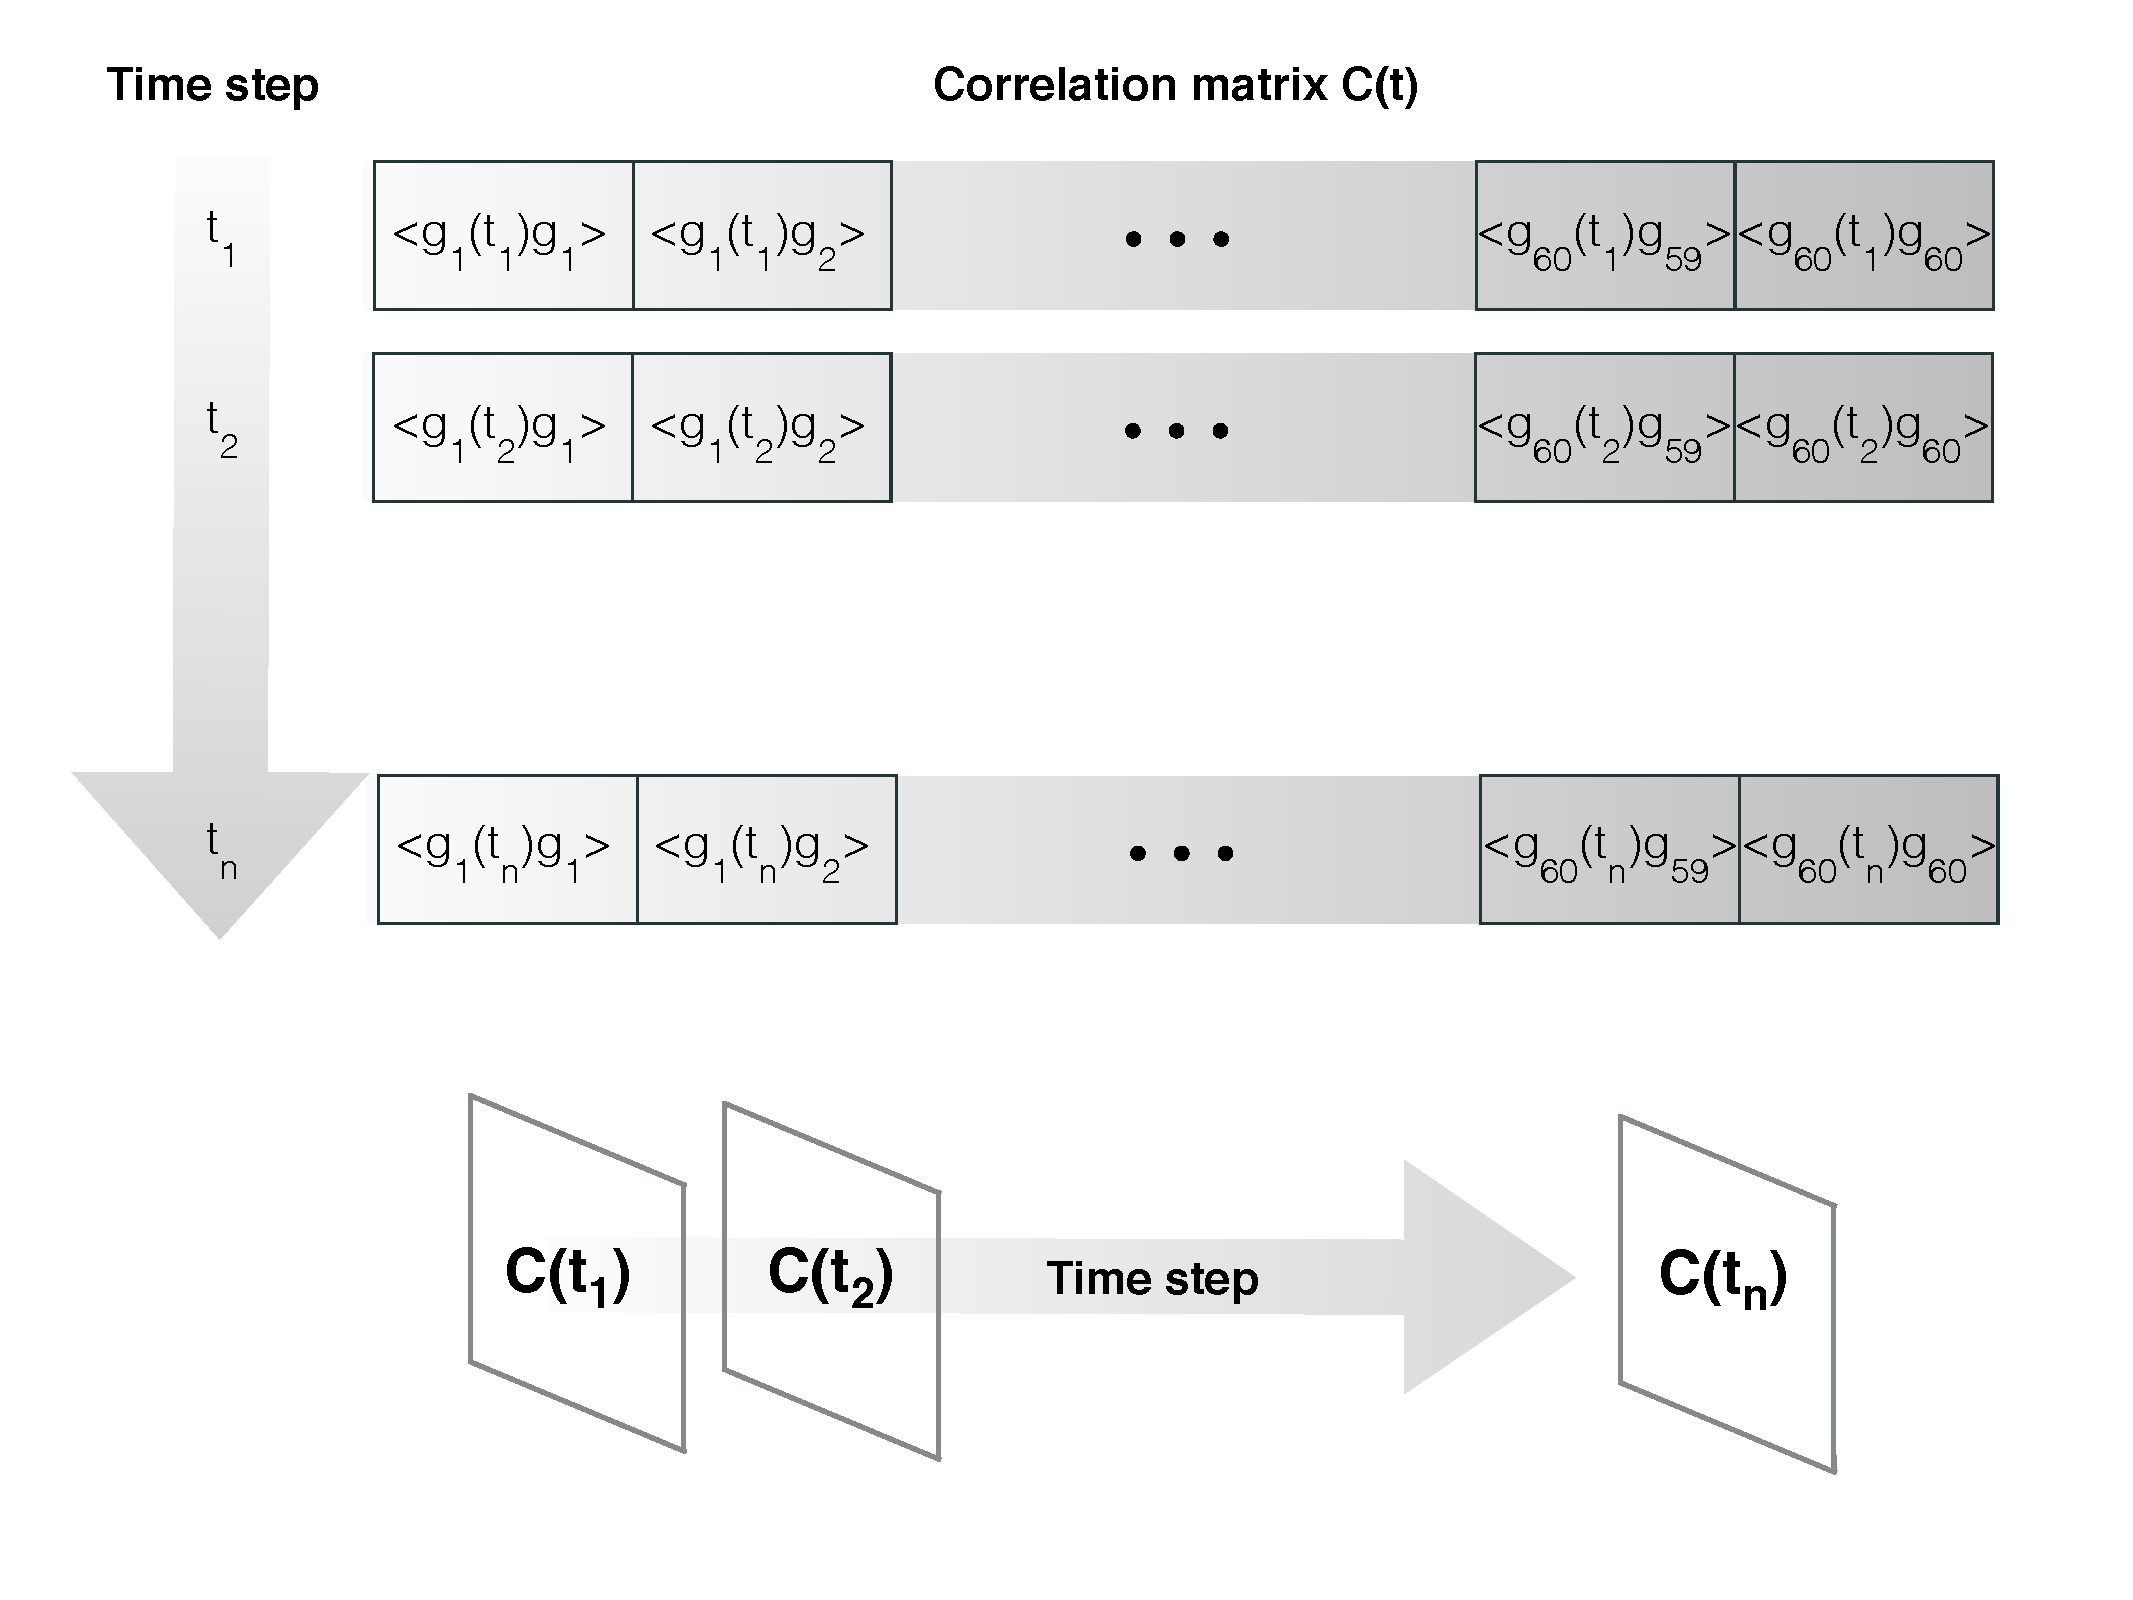
\includegraphics[width=\linewidth]{lammps-python}
%\end{figure}
% \end{frame}
 
 \begin{frame}{The correlation matrix $C(t)$ and its eigenvalues $\tilde{C}_{\mu\mu}$}
   \begin{itemize}
 \item<1->
   The correlation matrix $C(t)$ at $t=0$ (left) and $t=0.6$ (right)
\begin{figure}[h!]
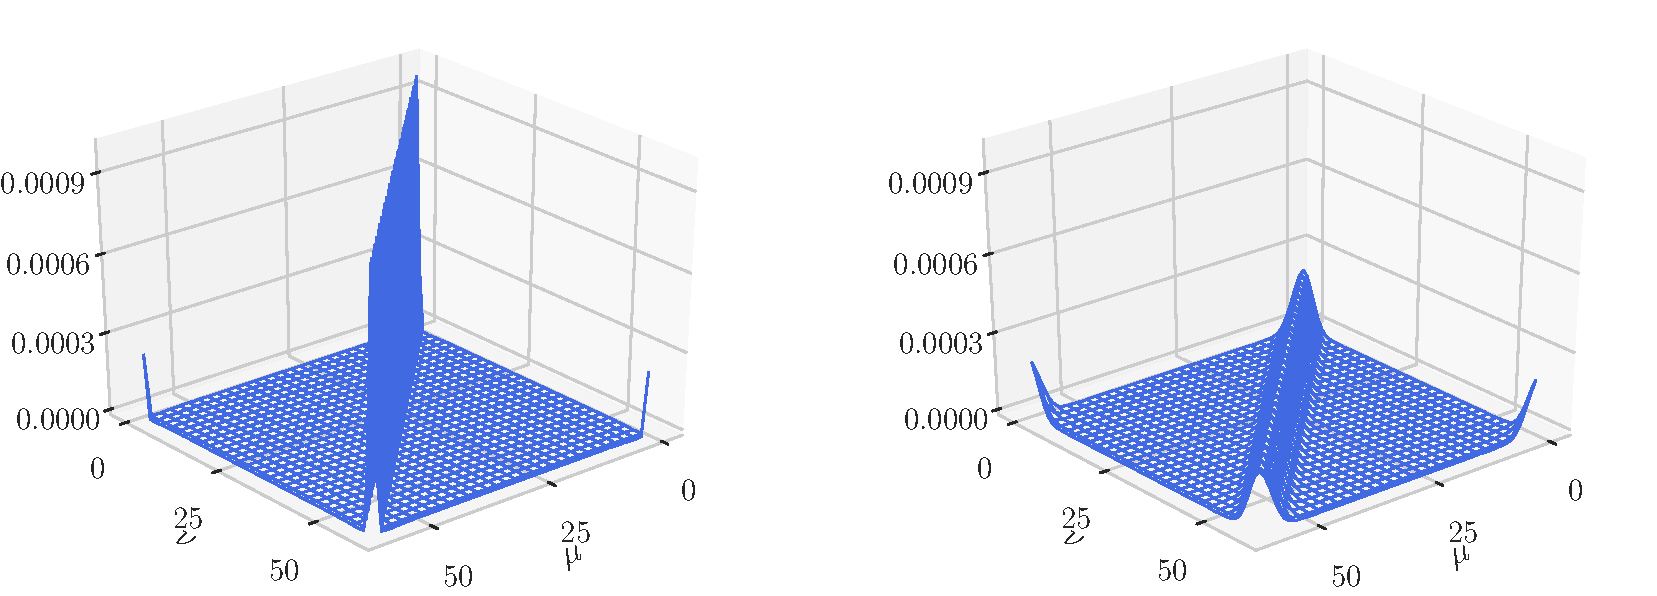
\includegraphics[width=\linewidth]{Ct-matrix-PBC}
\end{figure}
\item<2->  The evolution of the different eigenvalues $\tilde{C}_{\mu\mu}(t)$. %The horizontal  line  at  the   value  $2\times10^{-5}$,  signaling  the
  %threshold below which statistical errors give spurious results.
\begin{figure}[h!]
  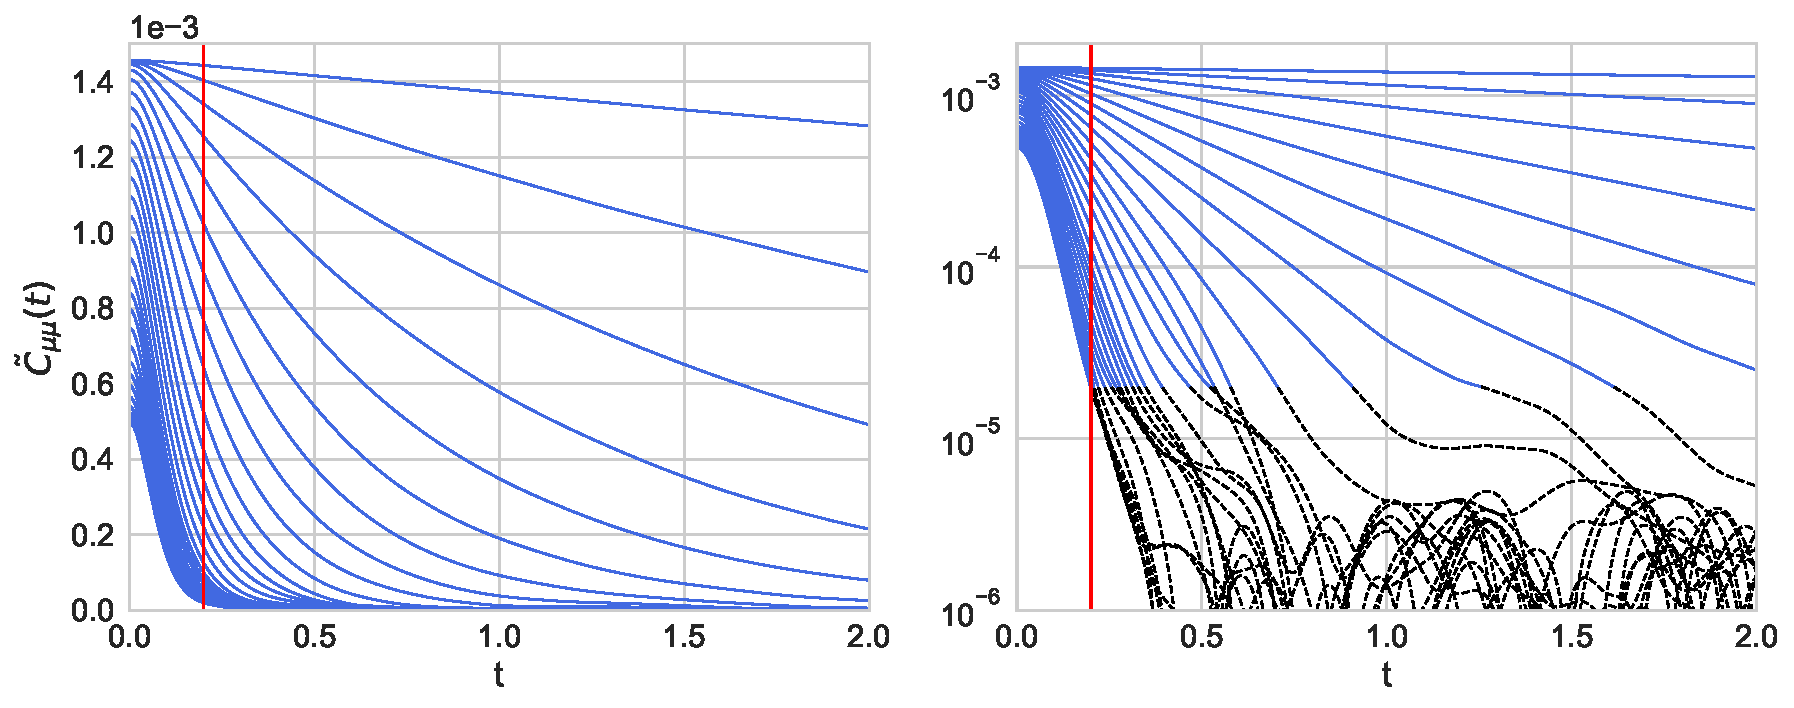
\includegraphics[width=\linewidth]{CtFourier-PBC-exp}
\end{figure}
\end{itemize}
\end{frame}

\begin{frame}{Validation of the Markovian approximation}
\begin{align}
  \tilde{\Lambda}_{\mu\mu}=-\frac{1}{\tilde{C}_{\mu\mu}(t)}\frac{d\tilde{C}_{\mu\mu}}{dt}(t)
  \nonumber
\end{align}
\begin{figure}[h!]
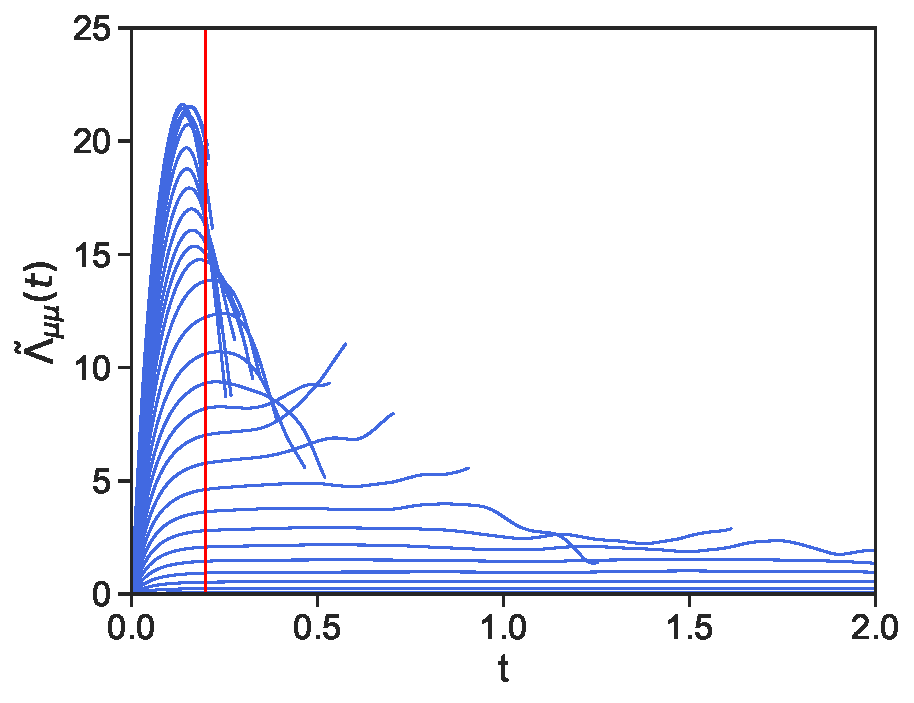
\includegraphics[width=\linewidth]{LambdatFourier-PBC-defense}
\end{figure}
  Left:
  in ascending  order times  go  from $t=0$  to $t=0.20$  in
  intervals of $0.02$.  Right: time evolution of $\tilde{\Lambda}_{\mu\mu}(t)$.
\end{frame}

\section{Markovian behaviour near solids}
\begin{frame}{The system and the CG variables}
\begin{itemize}
  \item The system
\begin{figure}
    \centering
    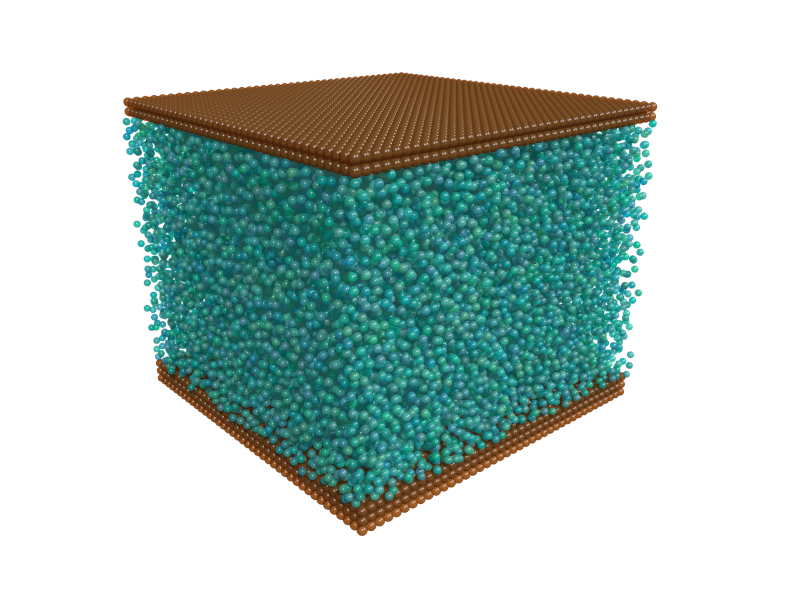
\includegraphics[width=0.45\linewidth]{PRL3_gold2_wo_layers_wo_diffuse}
    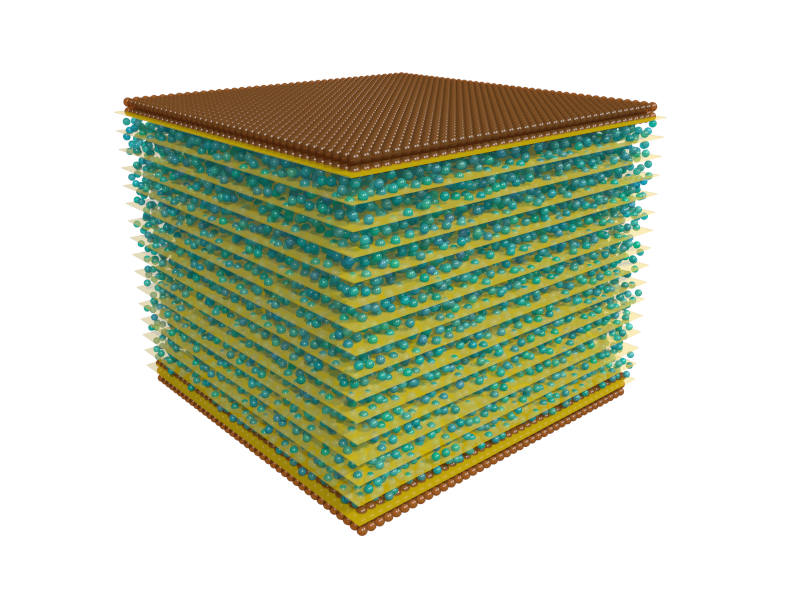
\includegraphics[width=0.45\linewidth]{PRL3_gold2_wo_diffuse}
\end{figure}
\item The CG variables and its correlation
\begin{align}
  \hat{\bf g}^x_\mu= \sum_i^N{\bf p}_i\delta_\mu({\bf q}_i), && 
  \hat{g}^T=(\hat{\bf   g}^x_1,\cdots,\hat{\bf  g}^x_{N_{\rm   bin}}), &&
  C(t)=\llangle \hat{g}(t) \hat{g}^T\rrangle 
\nonumber
\end{align}
\end{itemize}
\end{frame}

\begin{frame}{Simulation set up}
   \begin{itemize}
     \item Simulation of $28175$ fluid particles interacting with a LJ potential truncated at $\sigma=2.5$.
     \item Two solid walls in the $xy$ plane confine the fluid.  
     \item Box size $40x40x33$. 
     \item $dt=0.002$ in reduced units.
     \item Equilibration stage
       \begin{itemize}
         \item Langevin thermostat for $10^5$ timesteps: $T=2.0$, $\rho=0.6$.
         \item NVE microcanonical conditions for a further $10^5$ timesteps.
          \end{itemize}
        \item Production stage
       \begin{itemize}
         \item $12\times10^6$ timesteps.
         \item $z$ axis binned in $66$ bins $\mu$ $\boldsymbol{\Delta} {\bf z=0.5}\boldsymbol{\sigma}$ or $33$ bins $\mu$ $\boldsymbol{\Delta} {\bf z=2} \boldsymbol{\sigma}$.
         \item $g_{\mu}^x(t)$ recorded every $2$ timesteps. 
         \end{itemize}
     \end{itemize}
\end{frame}

\begin{frame}{Reciprocal space}
  \begin{itemize}
    \item Eigenvalues $\tilde{C}_{\mu}$ and eigenvectors $u_{\mu}$
\begin{align}
  C(t)&=\sum_\mu^{N_{\rm bin}}\tilde{C}_\mu(t) u_\mu(t) \otimes u_\mu^T(t)
\nonumber
\end{align}
    \item Unitary matrix $E(t)$
\begin{align}
  E^{-1}(t)\esc C(t)\esc E(t)=\tilde{C}(t)
\nonumber
\end{align}
\item We observed that $\dot{E}\simeq 0$.
\item The predictions of $C(t)$ in the reciprocal space
\begin{align}
  \tilde{C}_\mu(t)&=\exp\{-\tilde{\Lambda}_{\mu\mu} (t-\tau)\}  \tilde{C}_\mu(\tau)
  \nonumber
\end{align}
    \end{itemize}
\end{frame}

\begin{frame}{Thin bins ($\Delta z=0.5\sigma$)}
  \begin{itemize}
    \item $C_{\mu\nu}(t)$ for  $t=0$ (left) and $t=0.6$ (right).
\begin{figure}[h!]
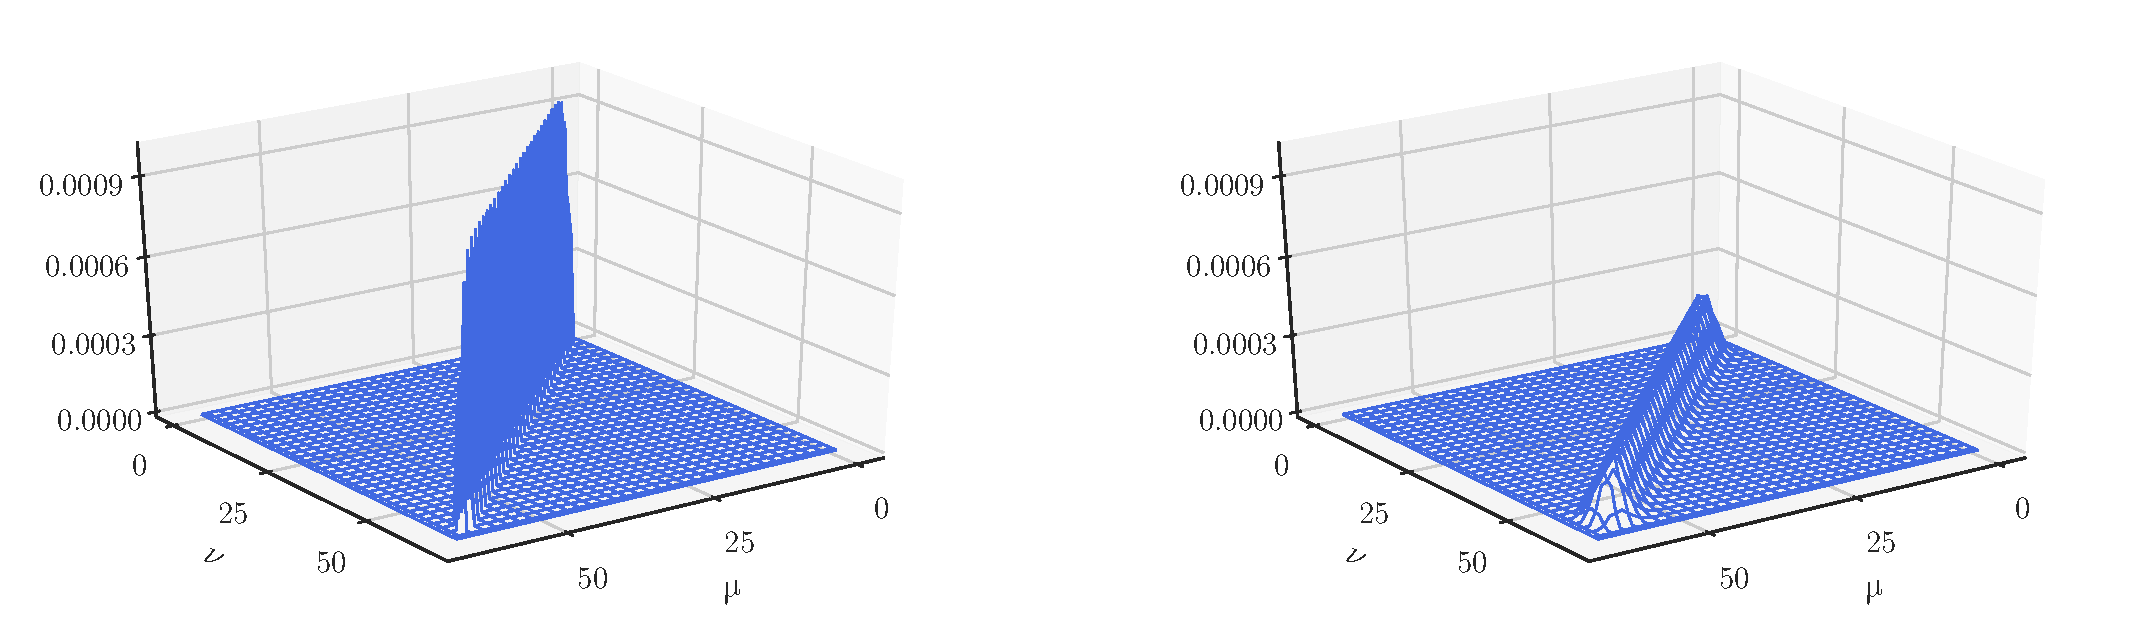
\includegraphics[width=\linewidth]{Ct-matrix-WALLS-66nodes}
\end{figure}
\item Evolution of different eigenvalues $\tilde{C}_{\mu\nu}(t)$
\begin{figure}[h!]
  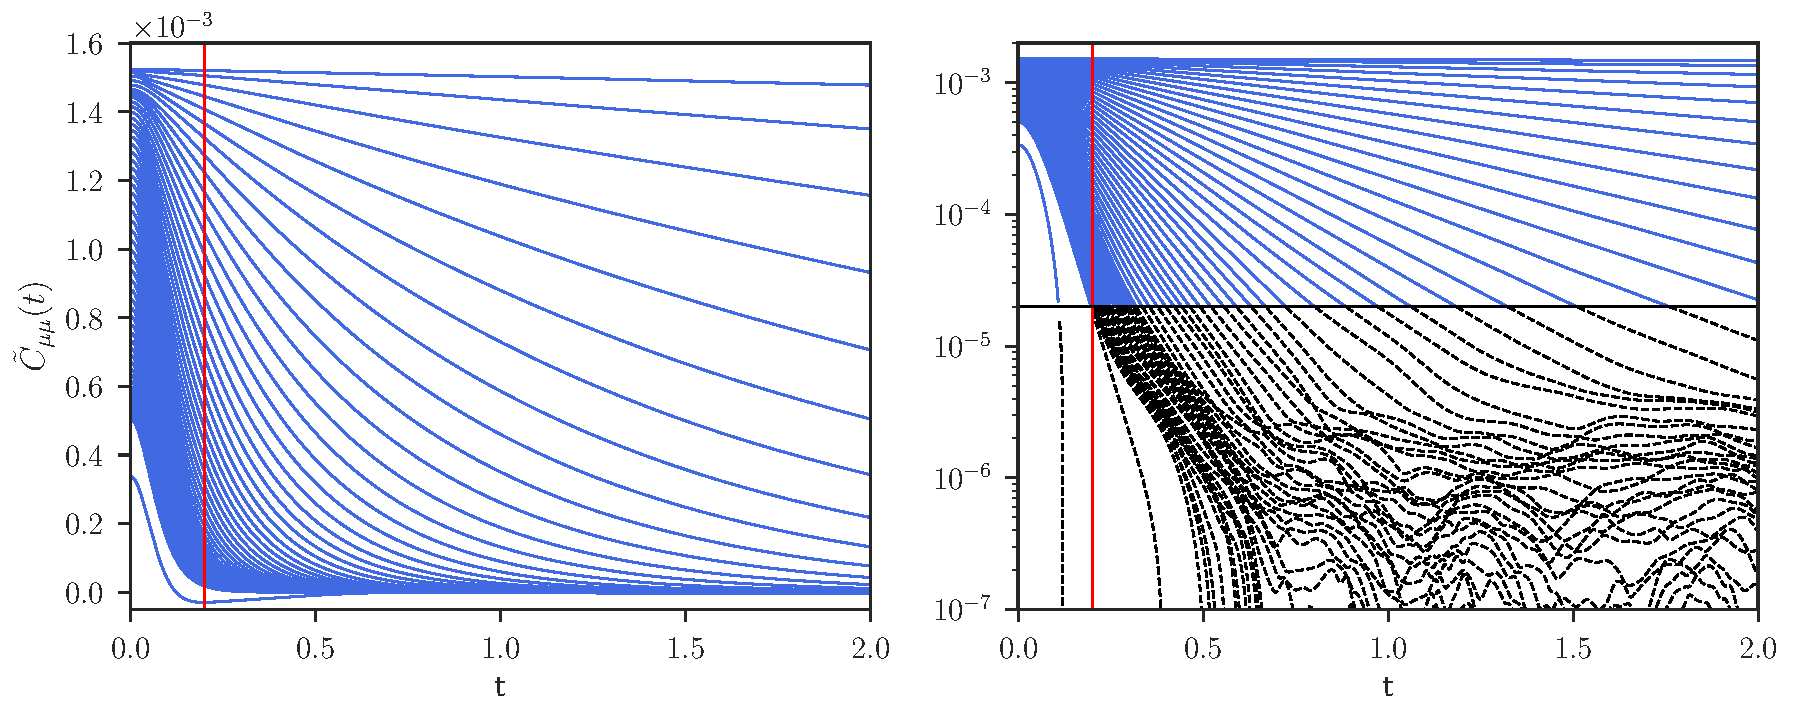
\includegraphics[width=\linewidth]{CtRec-WALLS-66nodes-exp}
\end{figure}
\end{itemize}
\end{frame}

\begin{frame}{Eigenvalues and eigenvectors near the walls ($\Delta z=0.5\sigma$)}
    The eigenvalues $\tilde{C}_{\mu}(t)$ of the correlation matrix $C(t)$ for $\mu=59,60$ which are identical and superimpose (left) and the corresponding eigenvectors $u_{\mu}$ in blue and orange, respectively (right).
  \begin{figure}[h!]
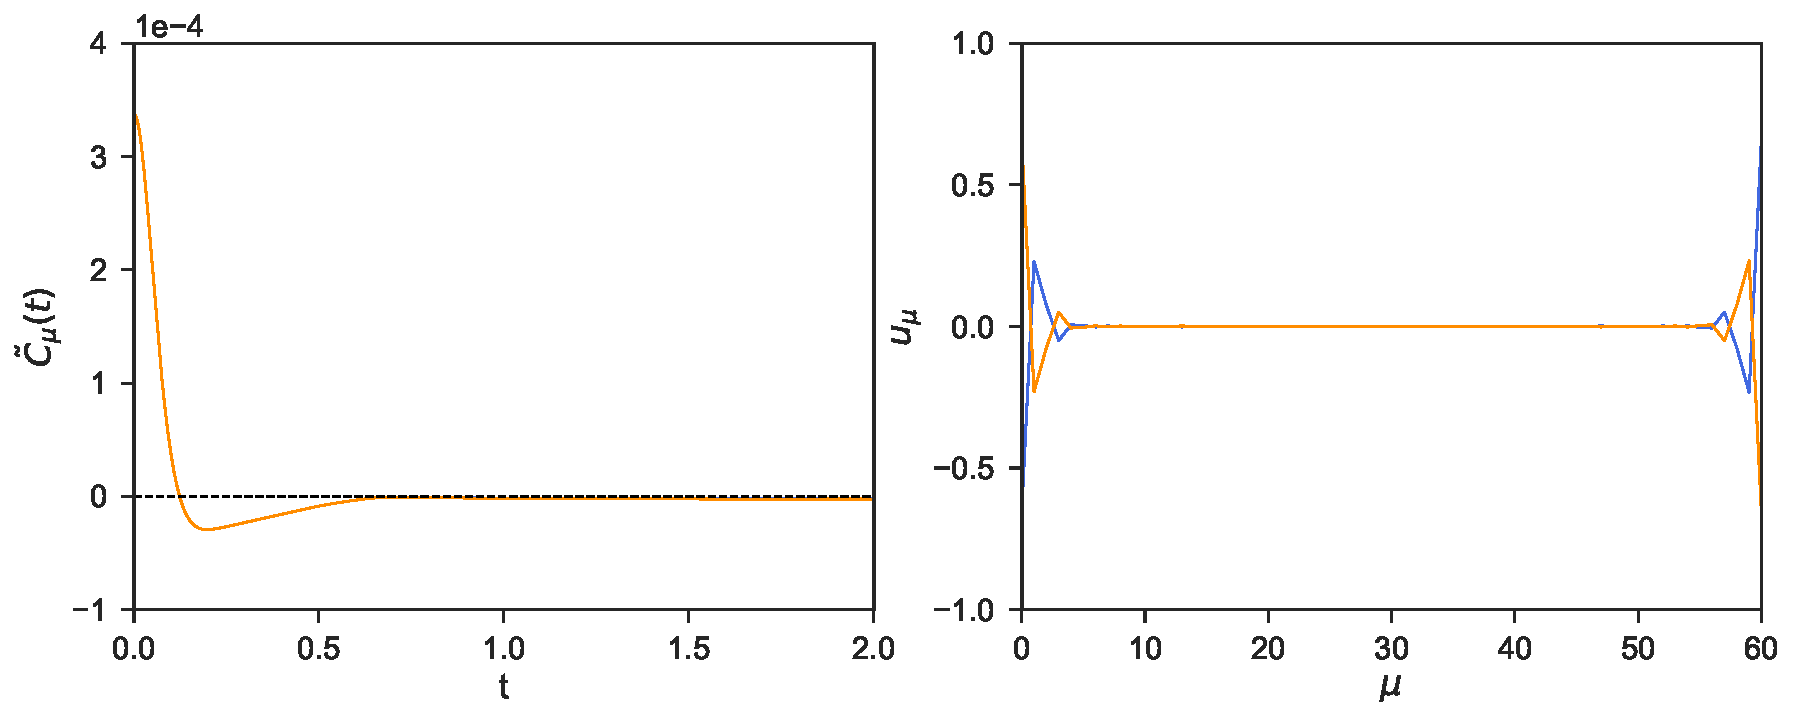
\includegraphics[width=1\linewidth]{EigenvaluesVectors-WALLS-66nodes}
\end{figure}
\end{frame}

\begin{frame}{$\tilde{\Lambda}(t)$ ($\Delta z=0.5\sigma$)}
Diagonal elements  $\tilde{\Lambda}_{\mu\mu}(t)$ of $\Lambda(t)$ in the reciprocal space. After a time $\tau=0.2$ we observe a nice plateau for the lower modes. 
\begin{figure}[h!]
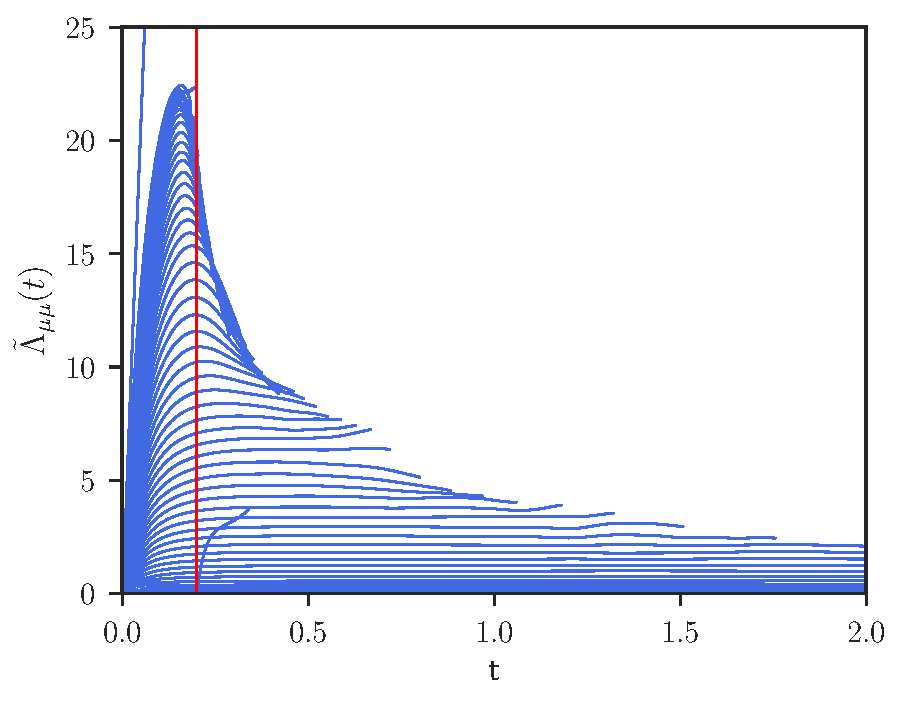
\includegraphics[width=0.7\linewidth]{LambdatRec-WALLS-66nodes}
\end{figure}
\end{frame}

\begin{frame}{Predicted correlations in the bulk ($\Delta z=0.5\sigma$)}
  In the middle of the canal the {\color{orange} predicted} correlation fits perfectly the {\color{blue} measured} correlation after a time $\tau=0.2$
\begin{figure}[h!]
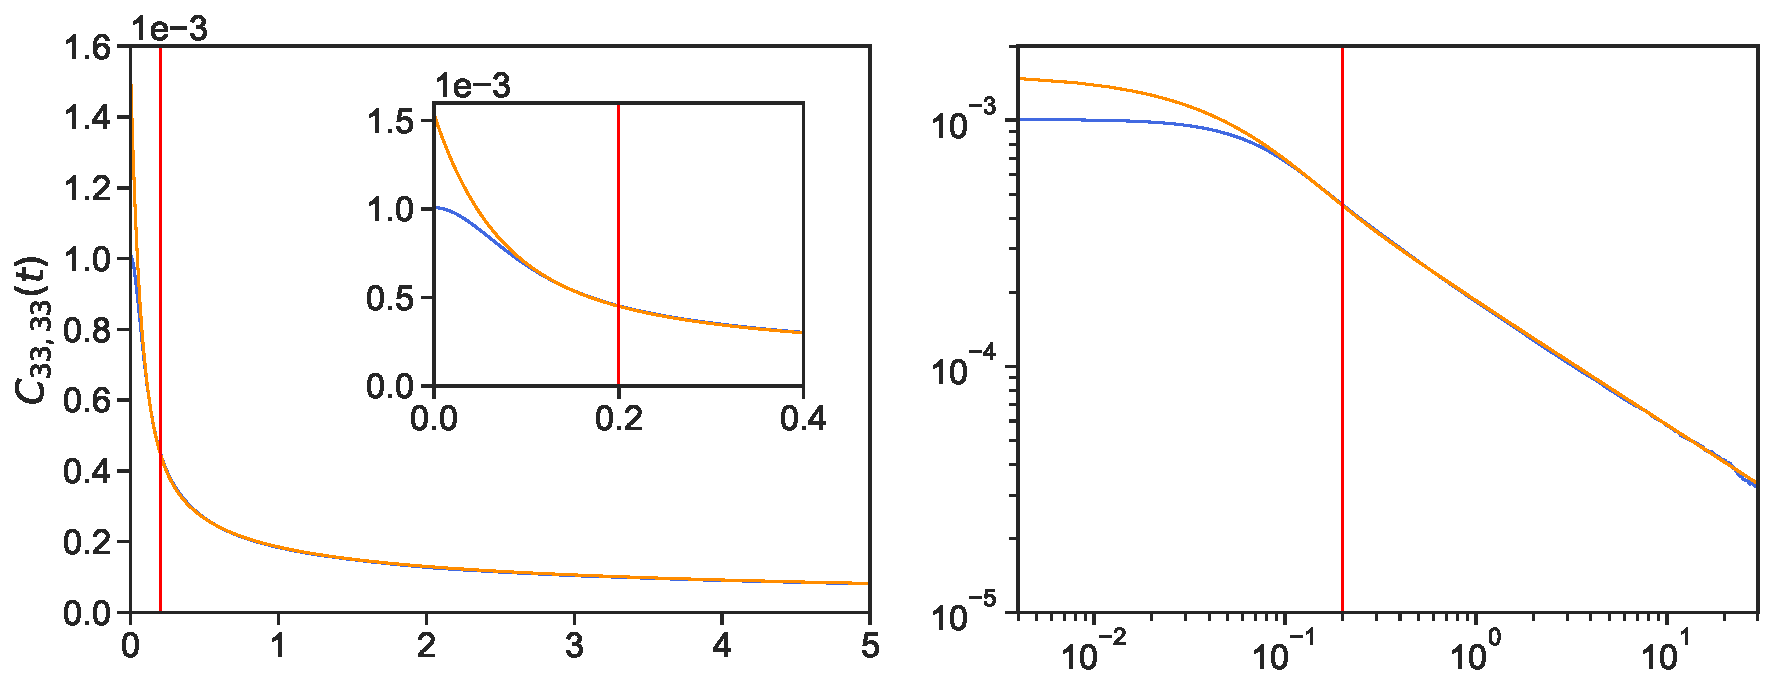
\includegraphics[width=\linewidth]{Predictions-canal-WALLS-66nodes-defense}
\end{figure}
\end{frame}

\begin{frame}{Predicted correlations near the walls ($\Delta z=0.5\sigma$)}
\begin{figure}[h!]
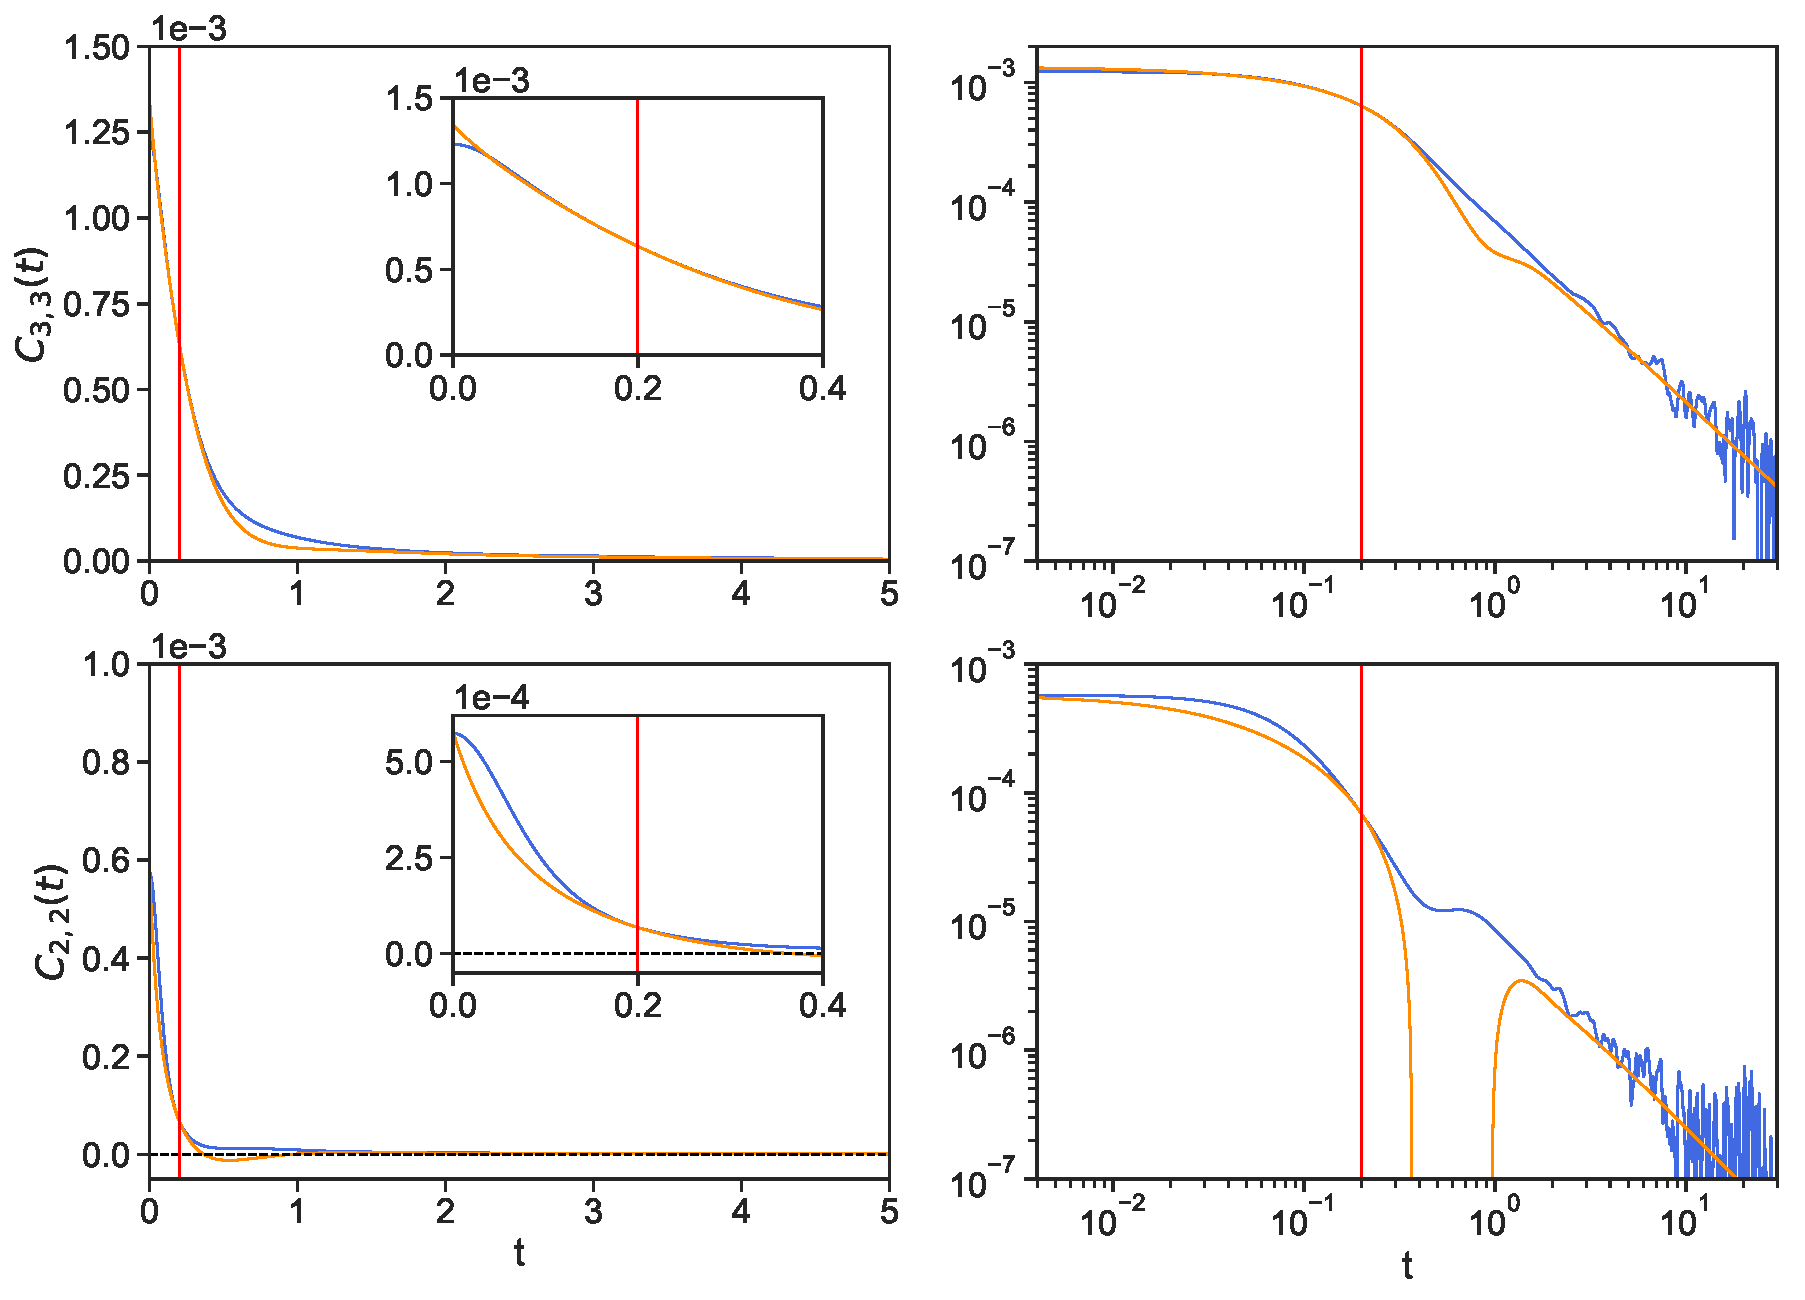
\includegraphics[width=\linewidth]{Predictions-WALLS-66nodes-defense}
\end{figure}
\end{frame}

\begin{frame}{From $\Delta z=0.5\sigma$ to $\Delta z=2\sigma$}
  \begin{itemize}
    \item We change the size of the bin
\begin{figure}[h!]
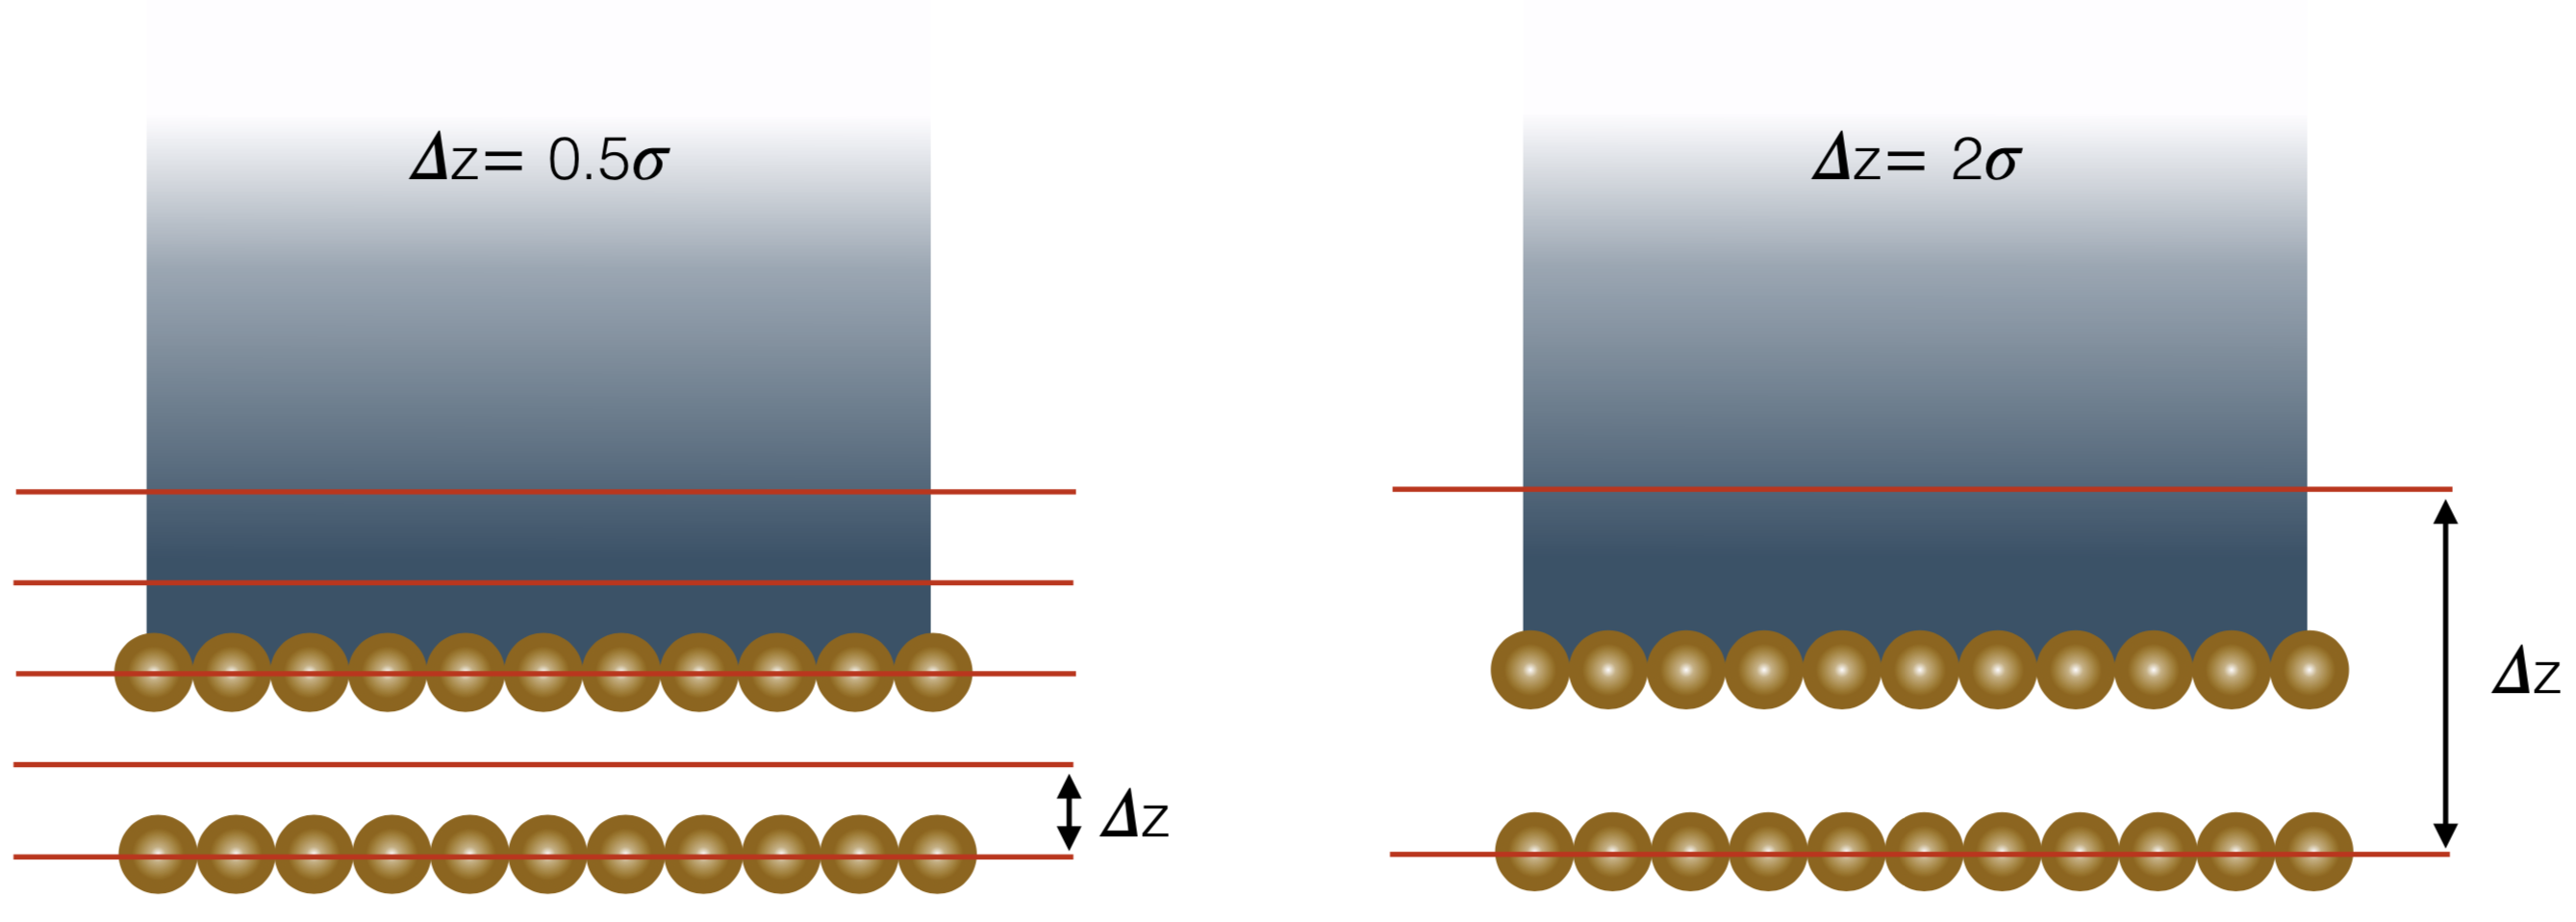
\includegraphics[width=0.9\linewidth]{bin_size}
\end{figure}
\item The thick bins do not capture the layering of the density field
\begin{figure}[h!]
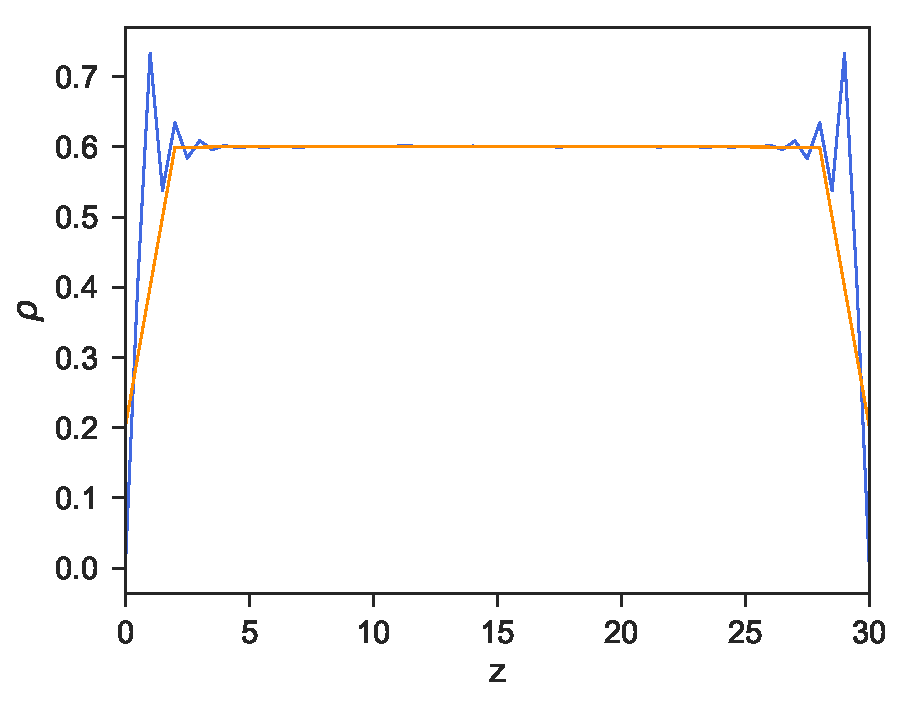
\includegraphics[width=0.47\linewidth]{DensityProfile-WALLS}
\end{figure}
  \end{itemize}
\end{frame}


\begin{frame}{Eigenvalues $\tilde{C}_{\mu\mu}(t)$ ($\Delta=2\sigma$)}
%Evolution of different eigenvalues $\tilde{C}_{\mu\nu}(t)$. Vertical line  at $t=\tau=0.3$.
\begin{figure}[h!]
  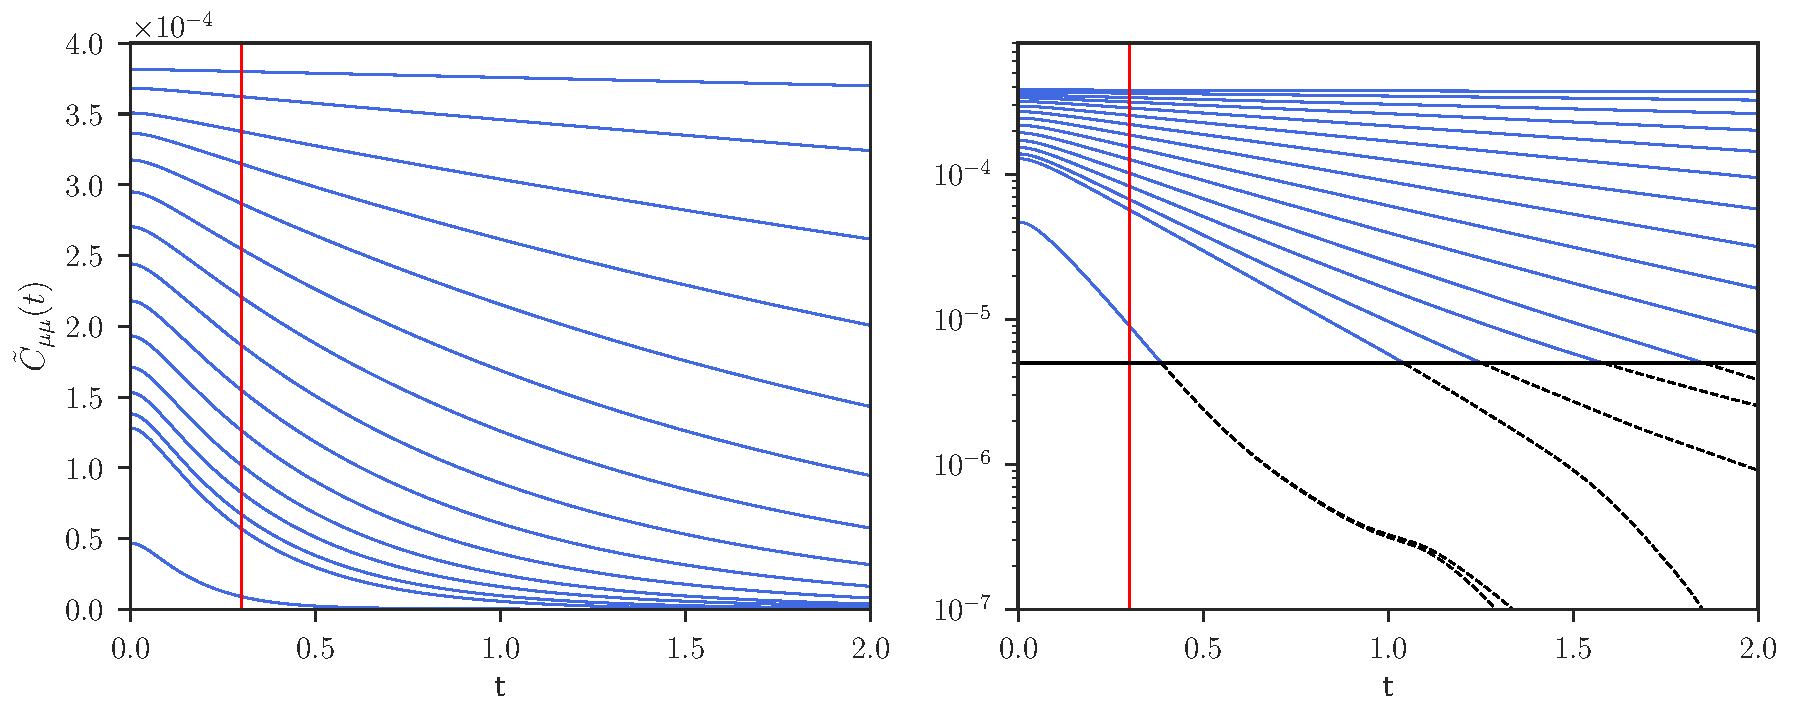
\includegraphics[width=0.87\linewidth]{CtRec-WALLS-17nodes-exp}
\end{figure}
\begin{figure}[h!]
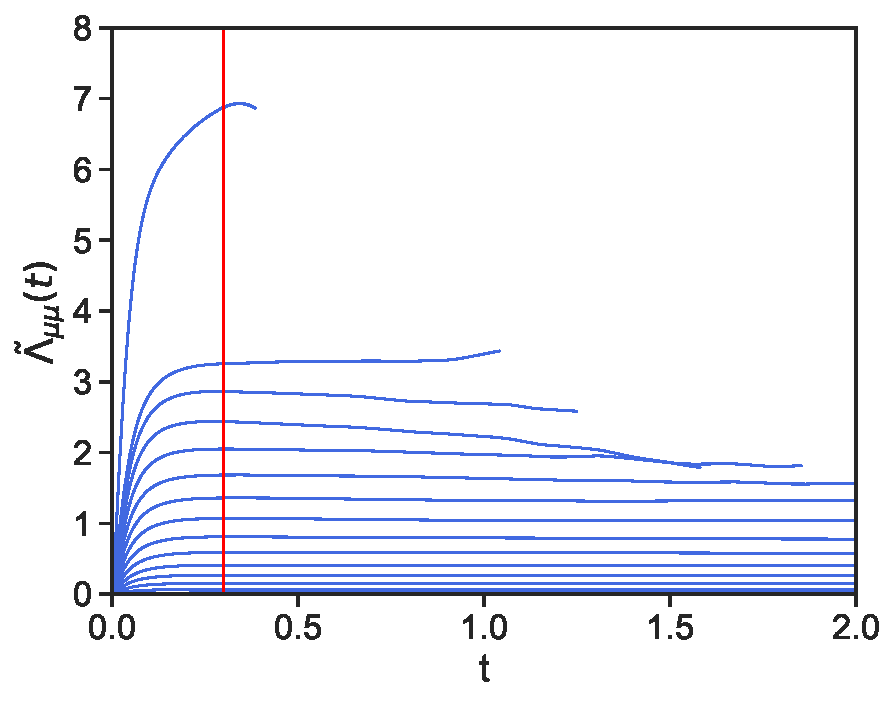
\includegraphics[scale=0.315]{LambdatRec-WALLS-17nodes}
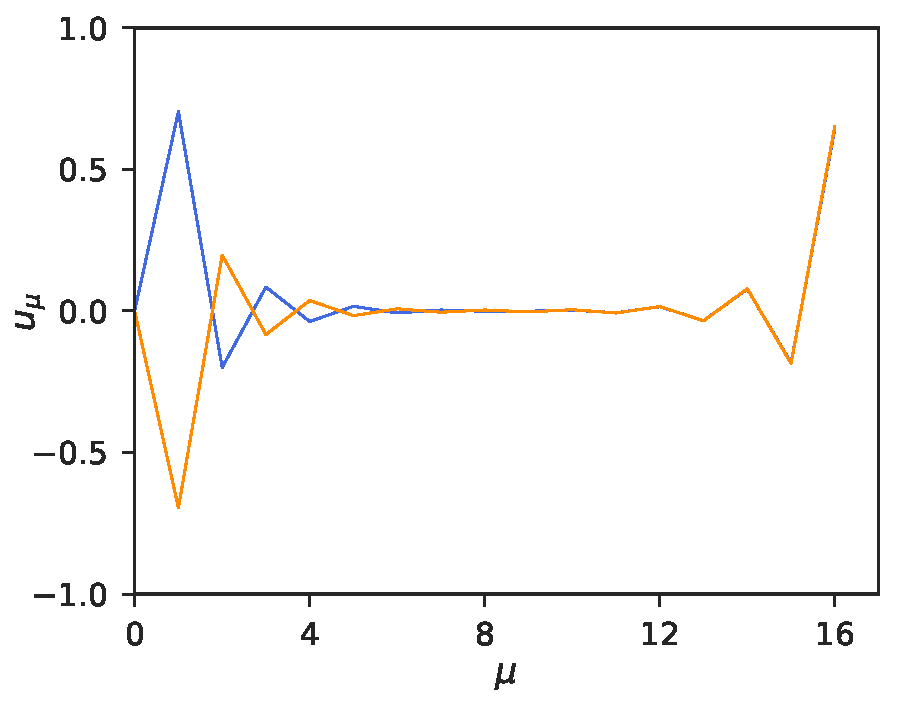
\includegraphics[scale=0.315]{Eigenvectors-WALLS-17nodes}
\end{figure}
\end{frame}

\begin{frame}{Predicted auto-correlations ($\Delta z=2\sigma$)}
\begin{figure}[h!]
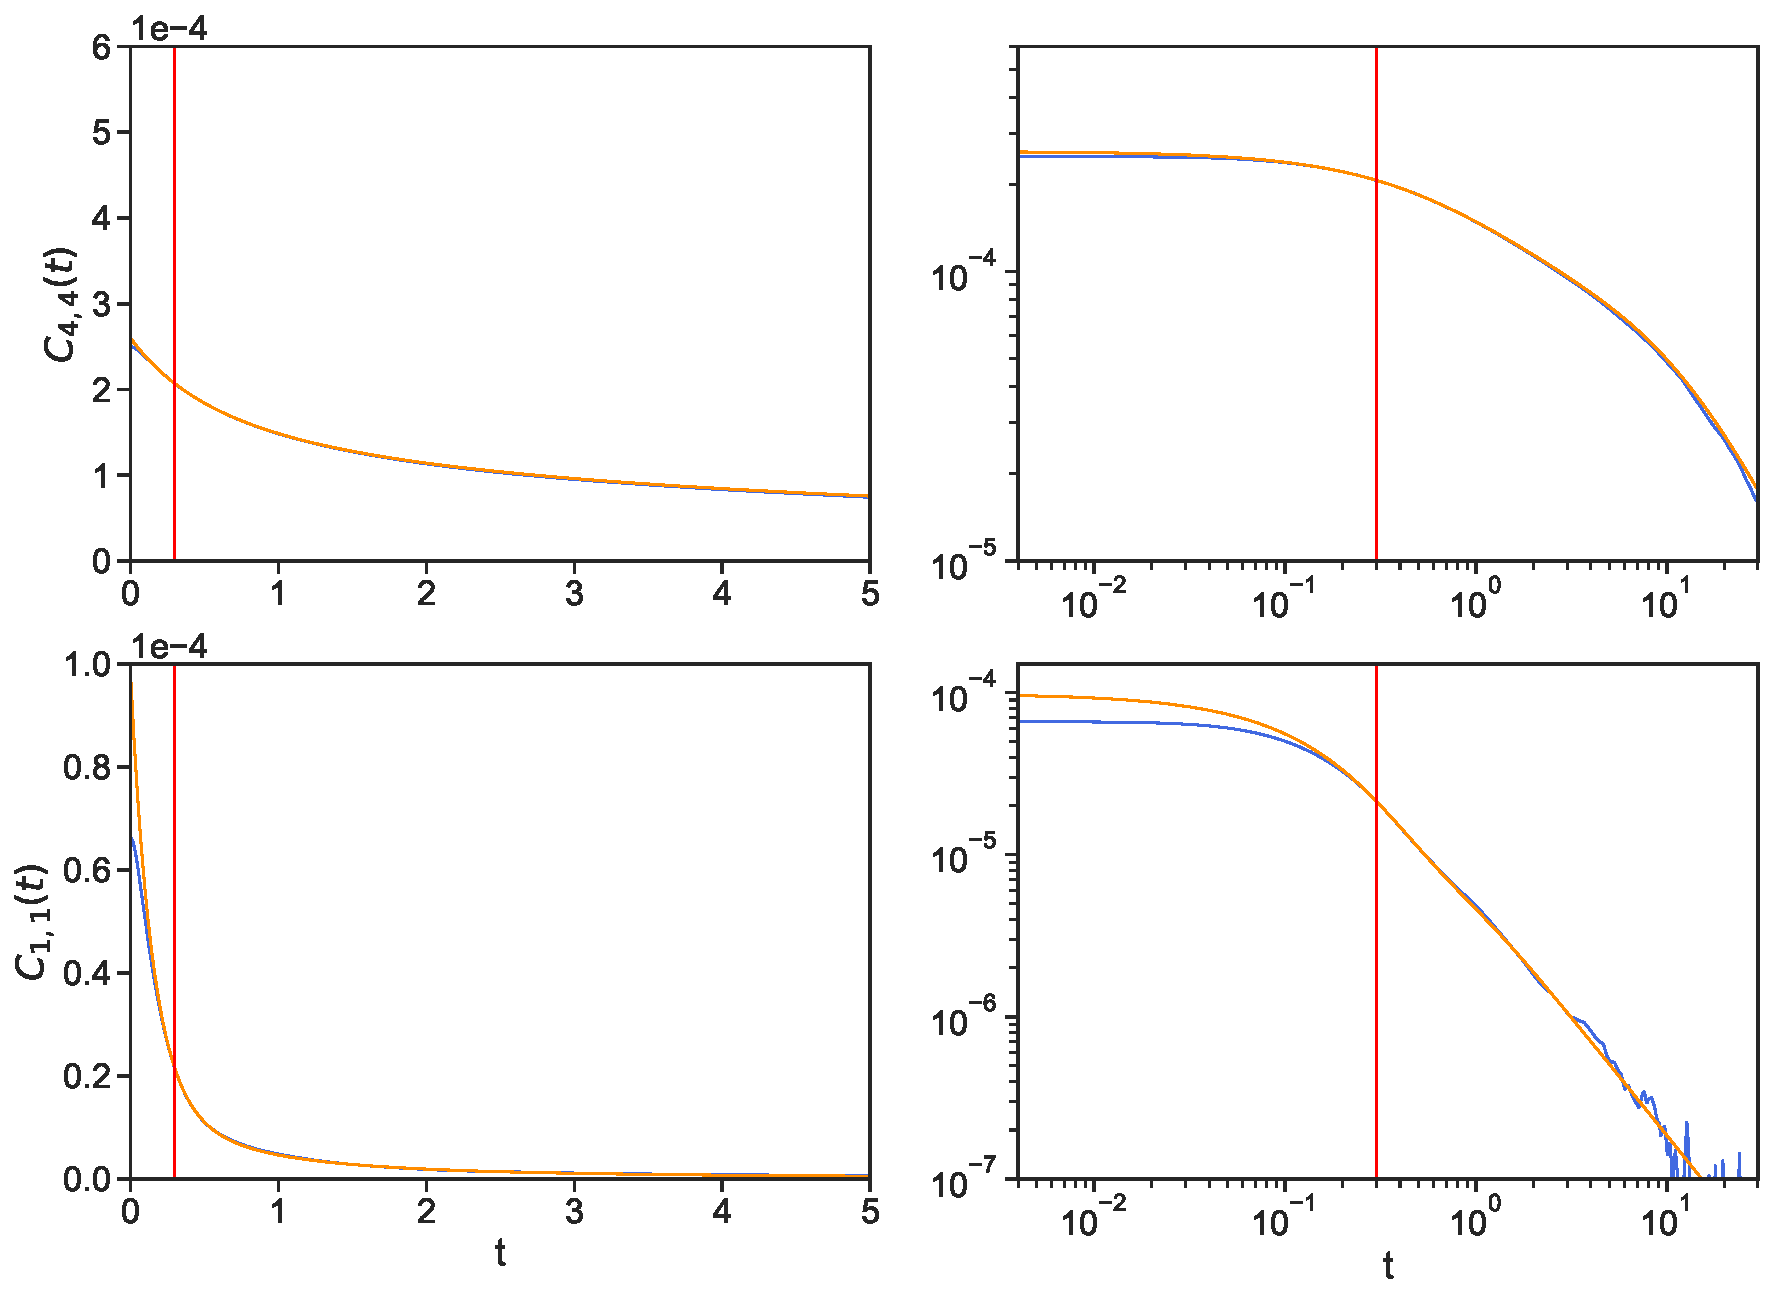
\includegraphics[width=\linewidth]{Predictions-WALLS-17nodes-defense}
\end{figure}
\end{frame}

\begin{frame}{Predicted cross-correlations ($\Delta z=2\sigma$)}
\begin{figure}[h!]
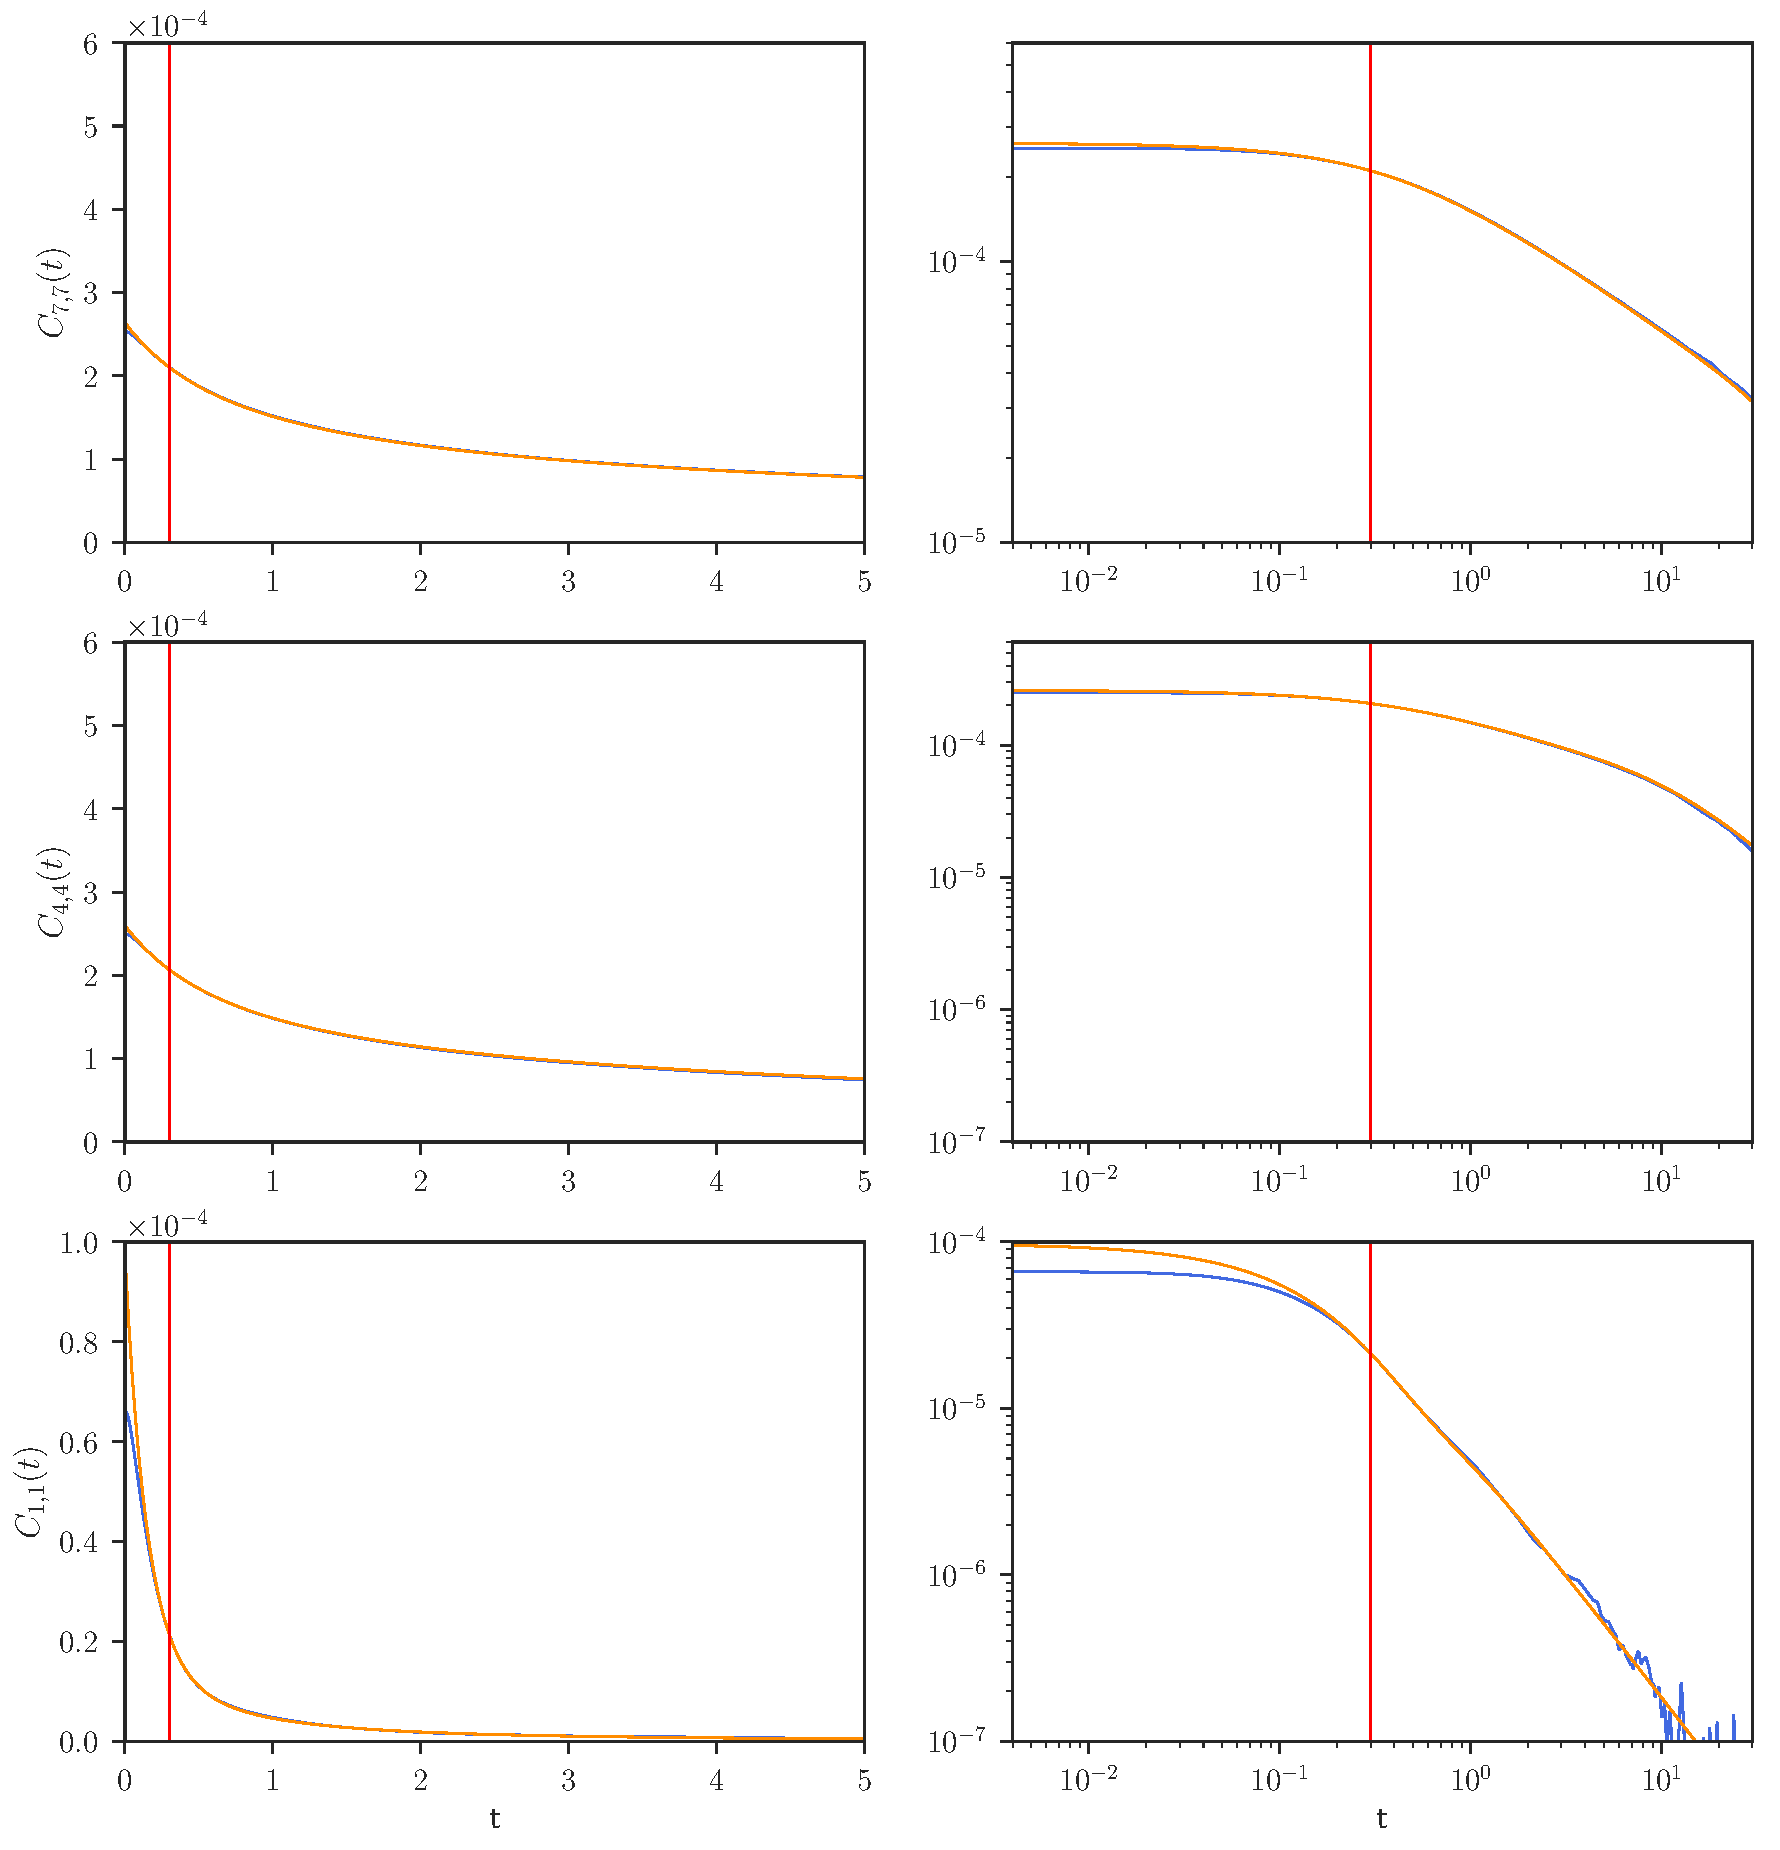
\includegraphics[width=\linewidth]{PredictionsCross-WALLS-17nodes}
\end{figure}
\end{frame}




\begin{frame}{Roadmap}
  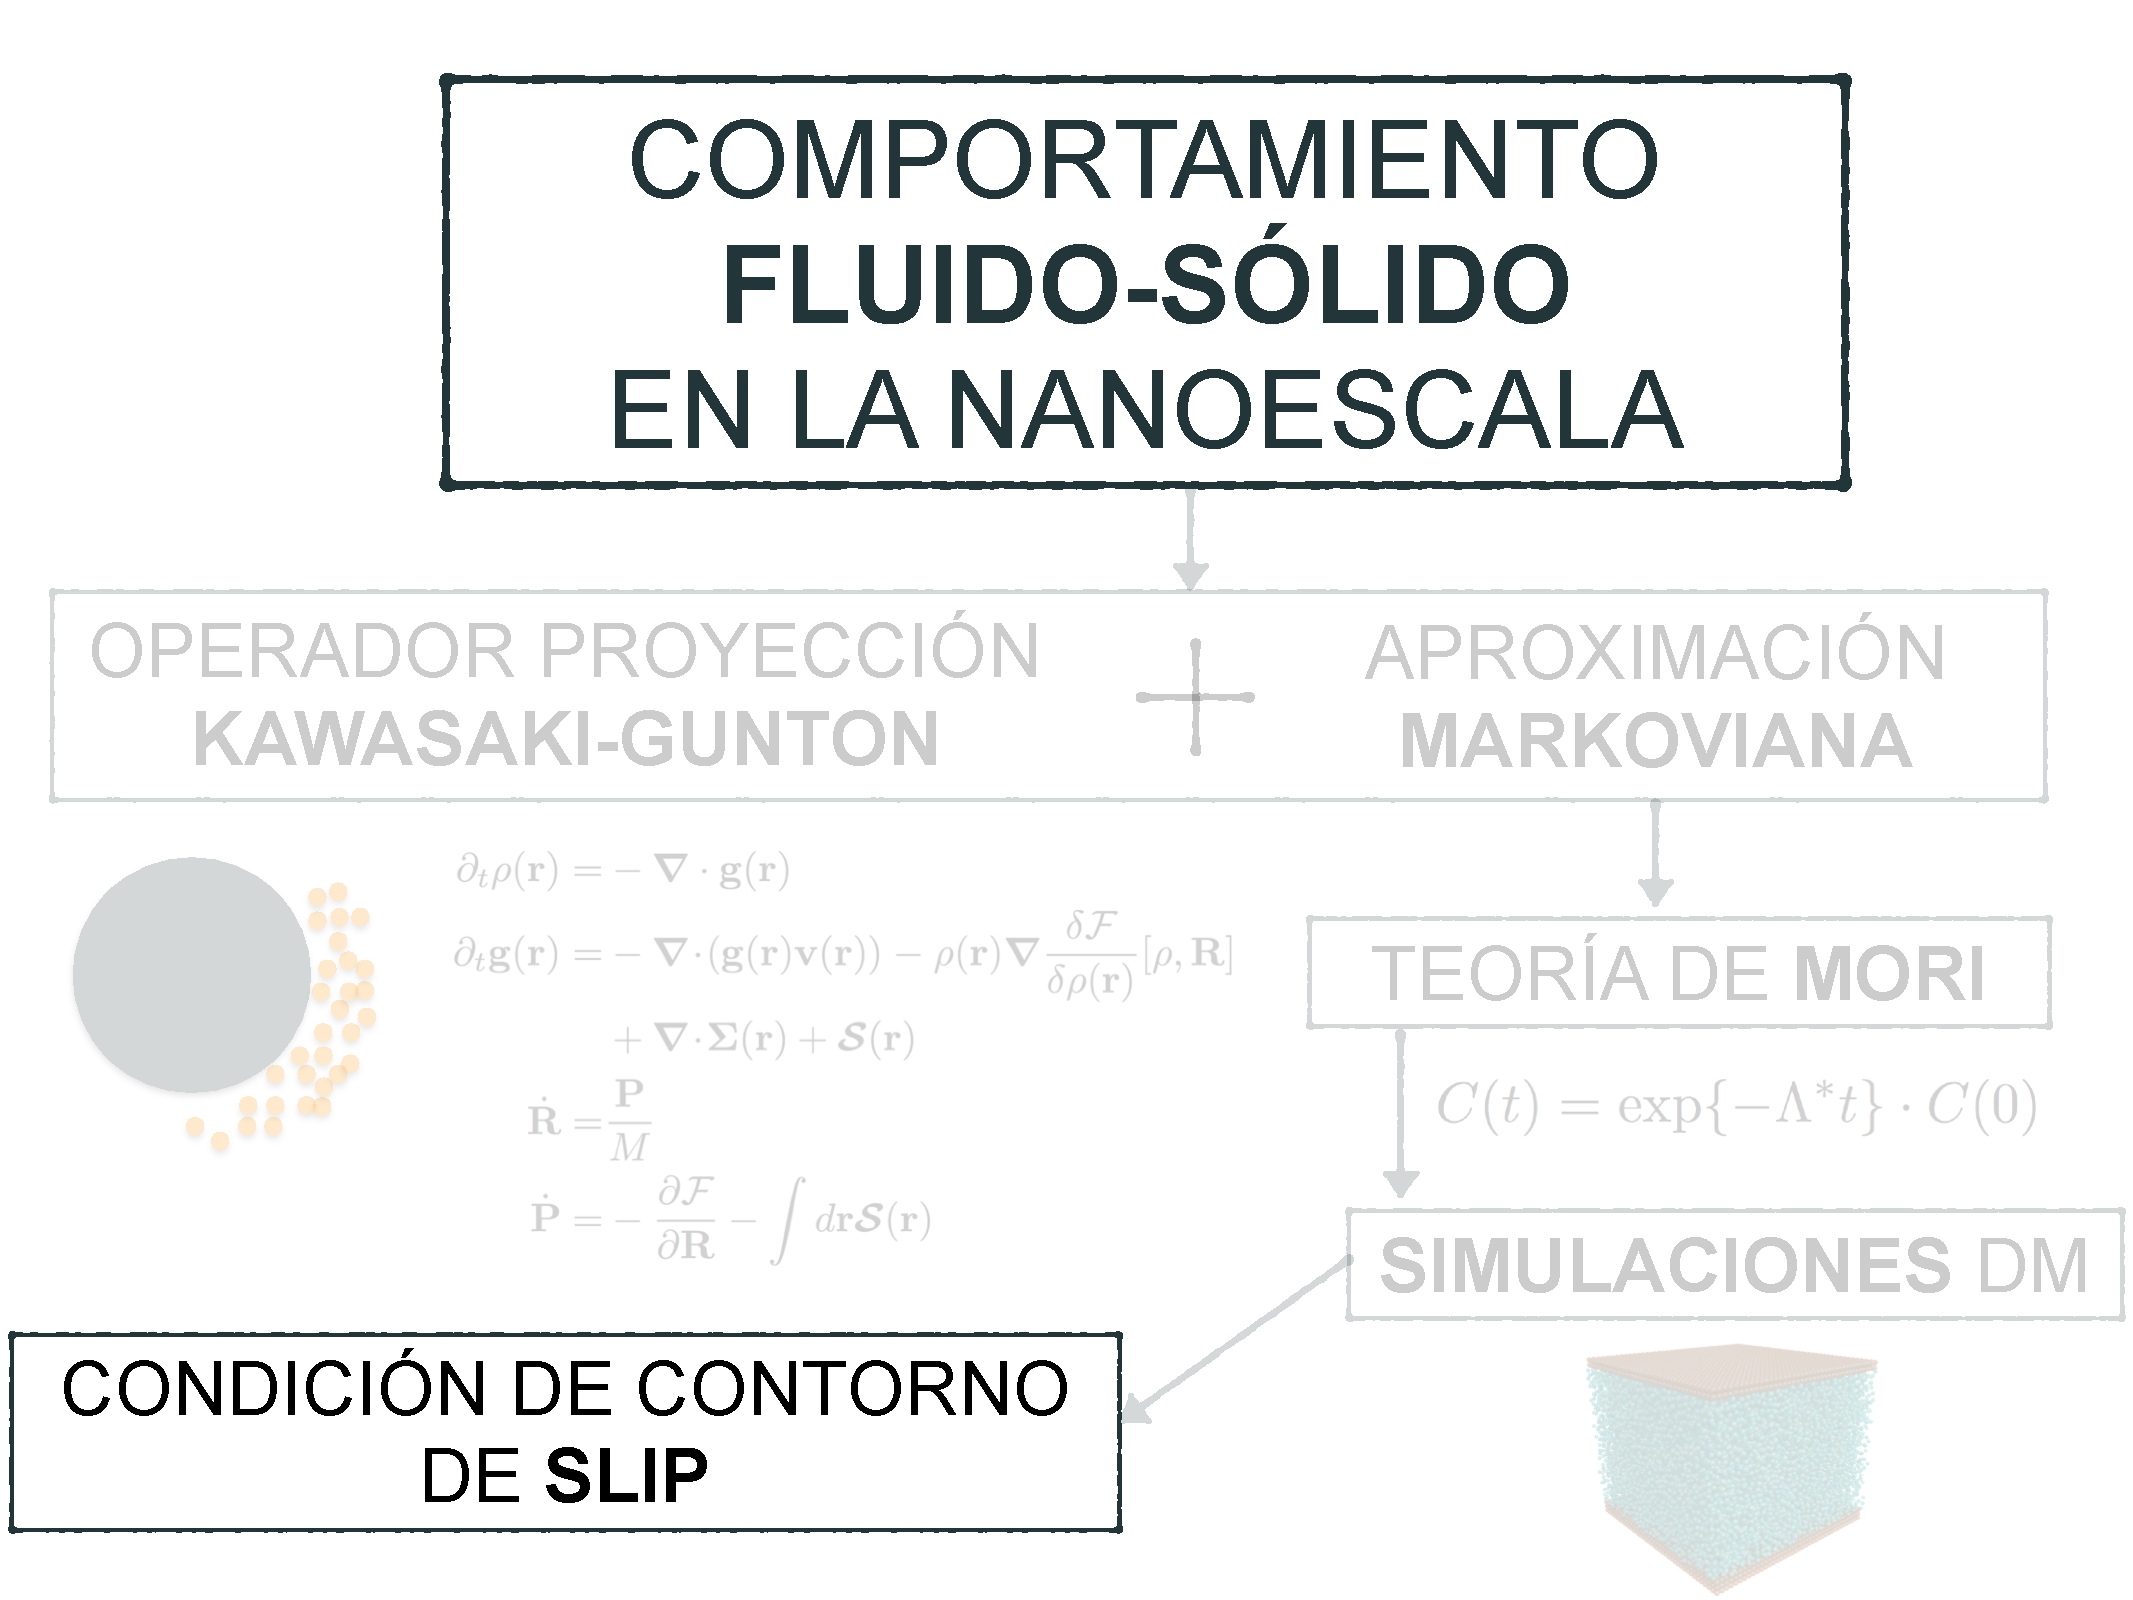
\includegraphics[width=\linewidth]{scheme-thesis-slip}
\end{frame}

\section{The slip boundary condition}
\begin{frame}{Strategy}
  \begin{enumerate}
    \item Compute the viscosity ($\eta$) and friction kernels ($G$, $H$, $\gamma$).
    \item Corrected Green-Kubo expression which avoid the plateau problem. 
    \item Predict the evolution of the average of the momentum profile, $g(t)$, with that transport kernels. 
    \item Navier slip boundary condition $\rightarrow$ slip length. 
    \item Check that the slip boundary condition is satisfied by a plug flow.
    %\item The slip lenght is independent on the channel width.
    \item Compare nonlocal and local theories. 
  \end{enumerate}
\end{frame}

\begin{frame}{Correlation matrix $C(t)$}
  \begin{itemize}
    \item We measure the correlation matrix $C(t)=\llangle \hat{g}(t) \hat{g}^T \rrangle$
%with $\hat{g}^T=(\hat{\bf g}^x_1,\cdots,\hat{\bf g}^x_{\rm bin})$.
\item  The time derivative of the correlation matrix
\begin{align}
  \frac{d}{dt}C(t)
=-  \int_0^t dt' \llangle i{\cal L}\hat{g}(t') i{\cal L}\hat{g}^T\rrangle
=-  k_BT M(t)
\nonumber
\end{align}
\item The Green-Kubo running integral 
\begin{align}
M(t)&= \frac{1}{k_BT}\int_0^t dt'\langle i{\cal L}\hat{g}(t')i{\cal L} \hat{g}^T\rangle
\nonumber
\end{align}
\item The time derivative of the momentum is 
\begin{align}
  i{\cal L}\hat{g}_\mu(z) &=\hat{F}_\mu(z)-\frac{\hat{\sigma}_\mu(z)-\hat{\sigma}_{\mu-1}(z)}{\Delta z}
\nonumber
\end{align}
where
$\hat{F}_\mu=\hat{\bf                   F}_\mu^x$                  and
$\hat{\sigma}_\mu=\hat{\boldsymbol{\sigma}}^{xz}_\mu$.
\item Therefore, the Green-Kubo running integral takes the form  
\begin{align}
{M}(t)&=F^T\esc{\eta}(t)\esc F+{G}(t)\esc F+F^T\esc{H}(t)+{\gamma}(t)
\nonumber
\end{align}
where $F$ is the bi-diagonal fordward finite difference operator.
  \end{itemize}
\end{frame}

\begin{frame}{The nonlocal transport matrices} 
\begin{align}
\eta_{\mu\nu}(t)
&=\frac{1}{k_BT}\int_0^t dt'
\left\langle \hat{\boldsymbol{\sigma}}^{xz}_{\mu}(t')\hat{\boldsymbol{\sigma}}^{xz}_{\nu}
\right\rangle
\nonumber\\
  G_{\mu\nu}(t)&=\frac{1}{k_BT}\int_0^t dt'
\left\langle\hat{\bf F}^x_\mu(t')
\hat{\boldsymbol{\sigma}}^{xz}_\nu
\right\rangle
\nonumber\\
H_{\mu\nu}(t)&=
\frac{1}{k_BT}\int_0^t dt'
\left\langle\hat{\boldsymbol{\sigma}}^{xz}_\mu(t')\hat{\bf F}^{x}_\nu\right\rangle
\nonumber\\
  \gamma_{\mu\nu}(t)
&=\frac{1}{k_BT}\int_0^t dt'
\left\langle 
\hat{\bf F}^{x}_\mu(t')
\hat{\bf F}^{x}_\nu\right\rangle
\nonumber
\end{align}
\end{frame}
\begin{frame}{The plateau problem}
$\eta_{10,10}(t)$ (middle of the channel), $\gamma_{1,1}$ (blue) and $\gamma_{2,2}$ (orange). 
\begin{figure}[]
  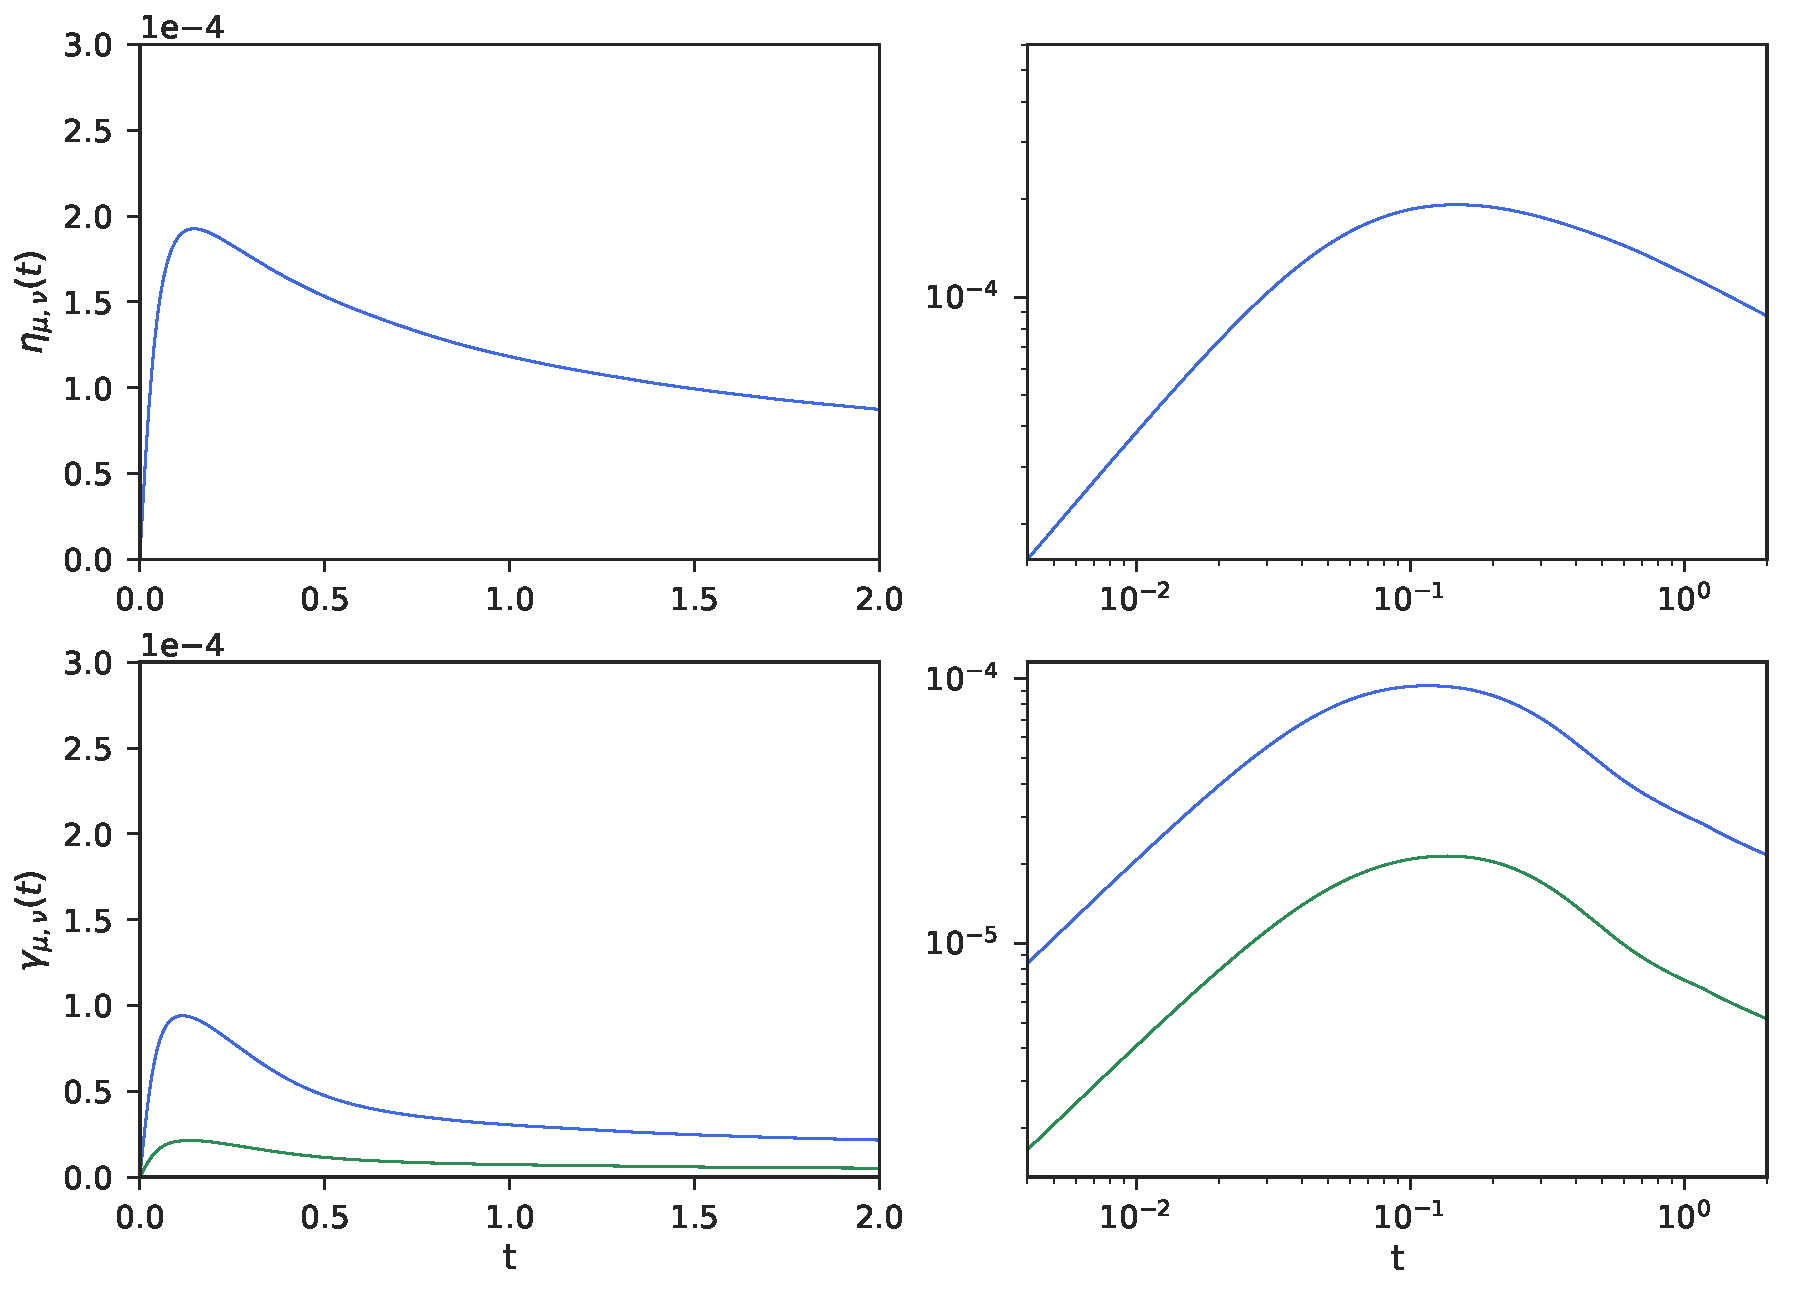
\includegraphics[scale=0.33]{NoPlateau-WALLS-17nodes}
\end{figure}
\end{frame}

\begin{frame}{Corrected Green-Kubo expression}
  \begin{itemize}
    \item Mori's theory and Markovian approximation 
      \begin{align}
        \frac{d}{dt}C(t)=-k_BT({\color{red}\cancel{L}} + M^*)\esc C^{-1}(0)\esc C(t)
        \nonumber
      \end{align}
    \item We also have $\frac{d}{dt}C(t)=-k_B T\esc M(t)$
    \item The \textit{corrected} Green-Kubo formula 
      %\begin{align}
       $ M^*=M(\tau)\esc C^{-1}(\tau)\esc C(0)$
      %\end{align}
      %where $c(\tau)=C^{-1}(0)\esc C(\tau)$
    \item The evolution of the correlation matrix
      \begin{align}
        \frac{d}{dt}C(t)=-k_BT\esc M(\tau)\esc {\color{red} C^{-1}(\tau)}\esc C(t)
        \nonumber
      \end{align}
    \item The evolution of the momentum field
      \begin{align}
        \frac{d}{dt}g(t)=-k_BT\esc M(\tau)\esc C^{-1}(\tau)\esc g(t)
        \nonumber
      \end{align}
    \item The evolution of the velocity field
      \begin{align}
        \frac{d}{dt}v(t)=-k_BT\esc M(\tau)\esc C^{-1}(\tau)\esc {\cal V}\esc \underbrace{C^{-1}(\tau)\esc C(0)\esc v(t)}_{\overline{v}(t)}
        \nonumber
      \end{align}
  \end{itemize}
\end{frame}

\begin{frame}{Plug flow simulation}
  \begin{itemize}
    \item Simulations to generate a nonequilibrium plug flow. 
    \item Add to the thermal velocity of each fluid atom the same velocity $\bf{V}$ 
\begin{figure}[]
  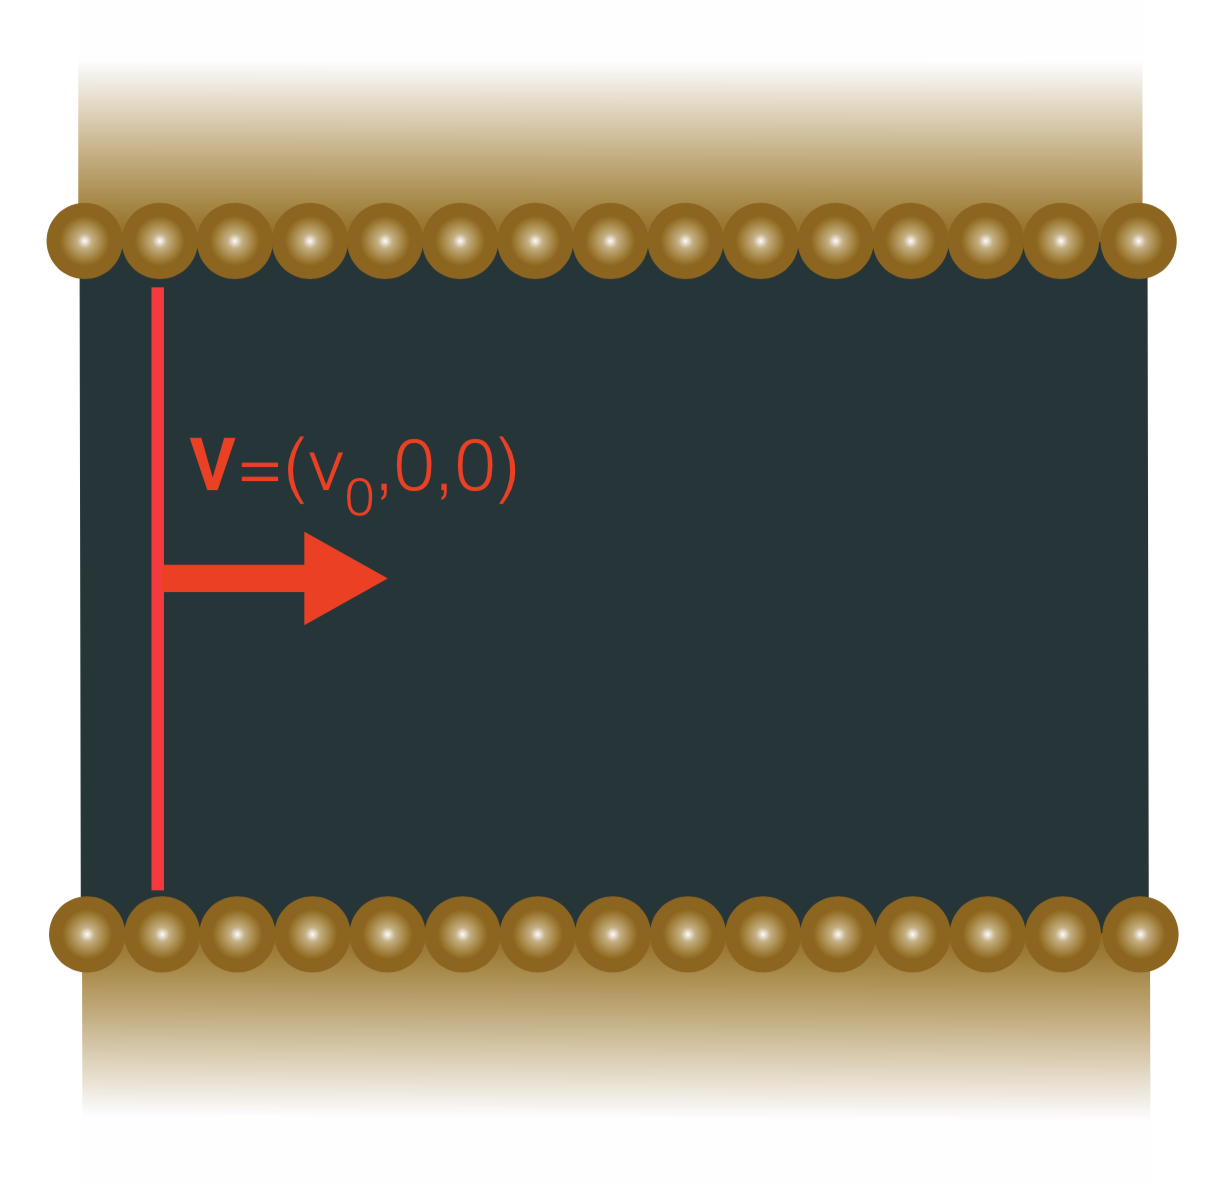
\includegraphics[width=0.3\linewidth]{plug_flow}
\end{figure}
\item Increase the kinetic energy $\rightarrow$ Increase the temperature. 
\item Rescale the resulting velocities in order to remain at the same temperature. 
\item Average over 5000 simulations with different initial configurations.
\item $g^x_{\mu})(t)$ recorded every 2 timesteps.  
  \end{itemize}
\end{frame}

\begin{frame}{Plug flow predictions}
  \begin{align}
    g(t)=\exp\{-\Lambda^* (t-\tau)\}\esc g(\tau)
    \nonumber
\end{align}
\begin{figure}[!h]
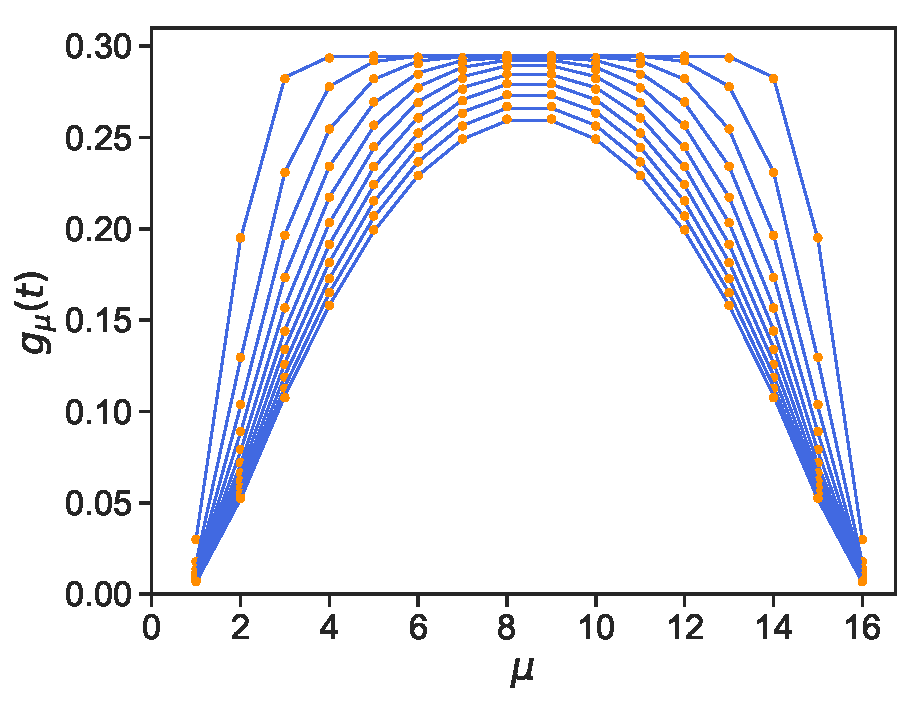
\includegraphics[width=0.5\linewidth]{gxtPredictions-17nodes-WALLS-defense1}
\end{figure}
The {\color{blue} measured momentum average} and the {\color{orange} predictions} for $\tau=0.3$ at times $t=1,3,...,21$ in descending order. 
\end{frame}

\begin{frame}{Plug flow predictions}
\begin{figure}[!h]
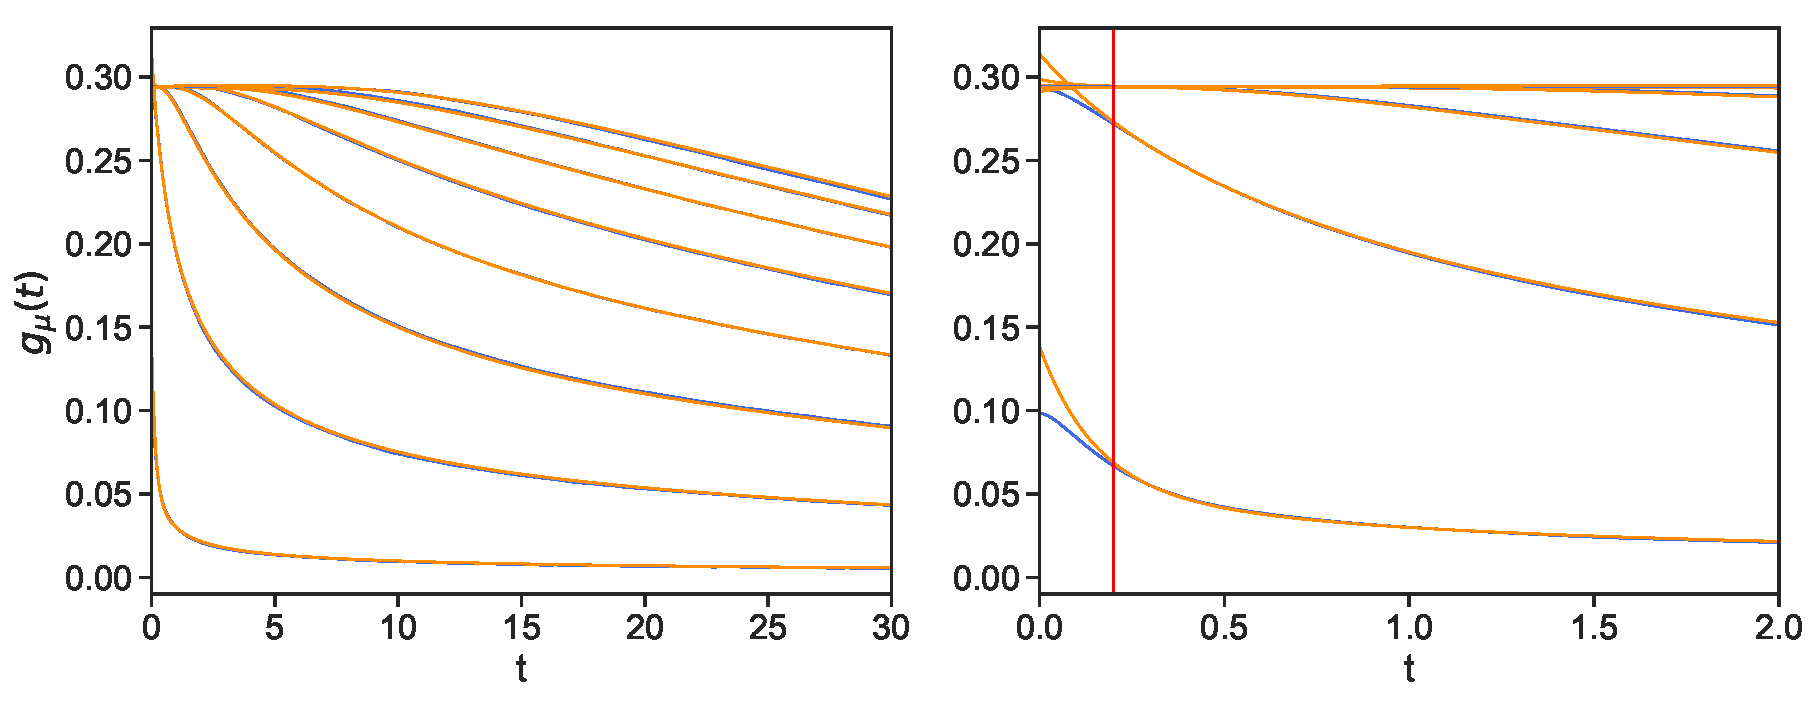
\includegraphics[width=\linewidth]{gxtPredictions-17nodes-WALLS-defense2}
\end{figure}
  \begin{itemize}
    \item The {\color{blue} measured momentum average} and the {\color{orange} predictions} for modes $\mu=1, 2,...,8$ in ascending order. Zoom at short times.
    \item Only after the tine in which the transport matrix reached a plateau, and hence a Markovian theory holds, it is expected that we get correct predictions. 
  \end{itemize}
\end{frame}

\begin{frame}{The boundary condition from pillbox argument}
Boundary slab of made of $B$ bins near one of the walls.
  \begin{enumerate}
    \item The momentum obeys the dynamics
      \begin{align}
        \frac{d}{dt}g(t)=-k_BT\esc M(\tau)\esc C^{-1}(\tau)\esc g(t)
        \nonumber
      \end{align}
\item The velocity field inside the boundary slab is linear
\begin{align}
\overline{\bf v}^x_{\mu}&=  \overline{\bf v}^x_{\rm wall}+\dot{\overline{\gamma}}_{\rm wall}(\mu\Delta z-z_{\rm wall})
\nonumber
\end{align}
      \begin{itemize}
        \item $z_{\rm wall}$: position of the wall. 
        \item $\overline{\bf v}^x_{\rm wall}$: velocity at $z_{\rm wall}$.
        \item $\dot{\overline{\gamma}}_{\rm wall}$: shear rate.
      \end{itemize}
\item The force on the boundary slab is vanishingly small. 
  \end{enumerate}
The Navier slip boundary condition and the slip length $\delta$
\begin{align}
\overline{\bf v}^x_{\rm wall}=\delta\dot{\overline{\gamma}}_{\rm wall}
  =\frac{\eta-G}{\gamma-H}\dot{\overline{\gamma}}_{\rm wall}
  \nonumber
\end{align}
\end{frame}

\begin{frame}{Linear approximation for the velocity and force on the slab}
\begin{figure}[!h]
  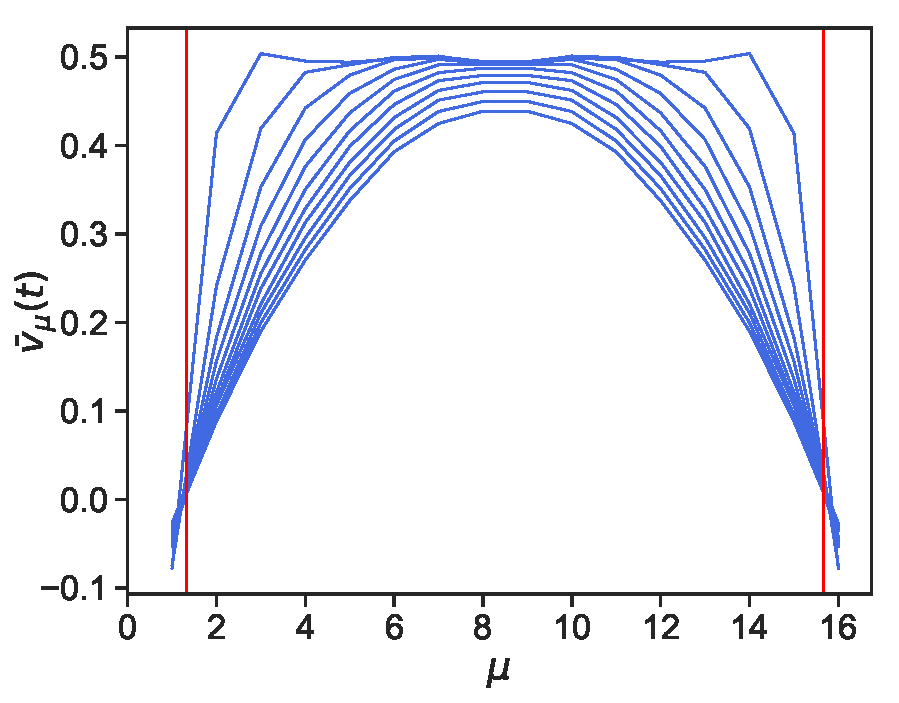
\includegraphics[width=0.5\linewidth]{vtCorrected-17nodes-WALLS-defense}
  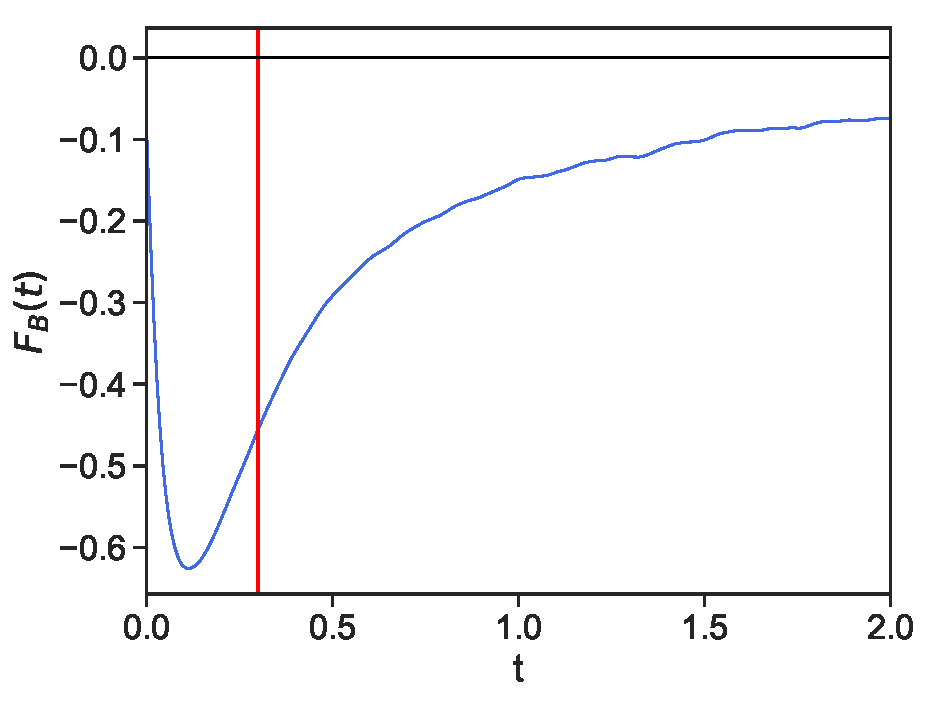
\includegraphics[width=0.5\linewidth]{checkMecBalance-17nodes-WALLS-defense}
\end{figure}
  \begin{itemize}
    \item The linear approximation for the velocity depends on the width of the boundary slab $B$. We choose $B=2$.\\
\item The force on the slab boundary vanishes for times larger than $t=2$.
  \end{itemize}
\end{frame}

\begin{frame}{Validation of the slip boundary condition}
  \begin{itemize}
    \item The slip length is measured from 
      %$\overline{\bf v}_{\rm wall}(t)$ and $\dot{\overline{\gamma}}_{\rm wall}$
%\begin{align}
 $\delta(t)=\frac{\overline{\bf v}^x_{\rm wall}(t)}{\dot{\overline{\gamma}}_{\rm wall}(t)}$
%\nonumber
%\end{align}
\item The slip lenght has to be constant according to 
  %\begin{align}
  $\delta =\frac{\eta -G}{\gamma-H}$
    %\nonumber
  %\end{align}
  \end{itemize}
  \begin{figure}[]
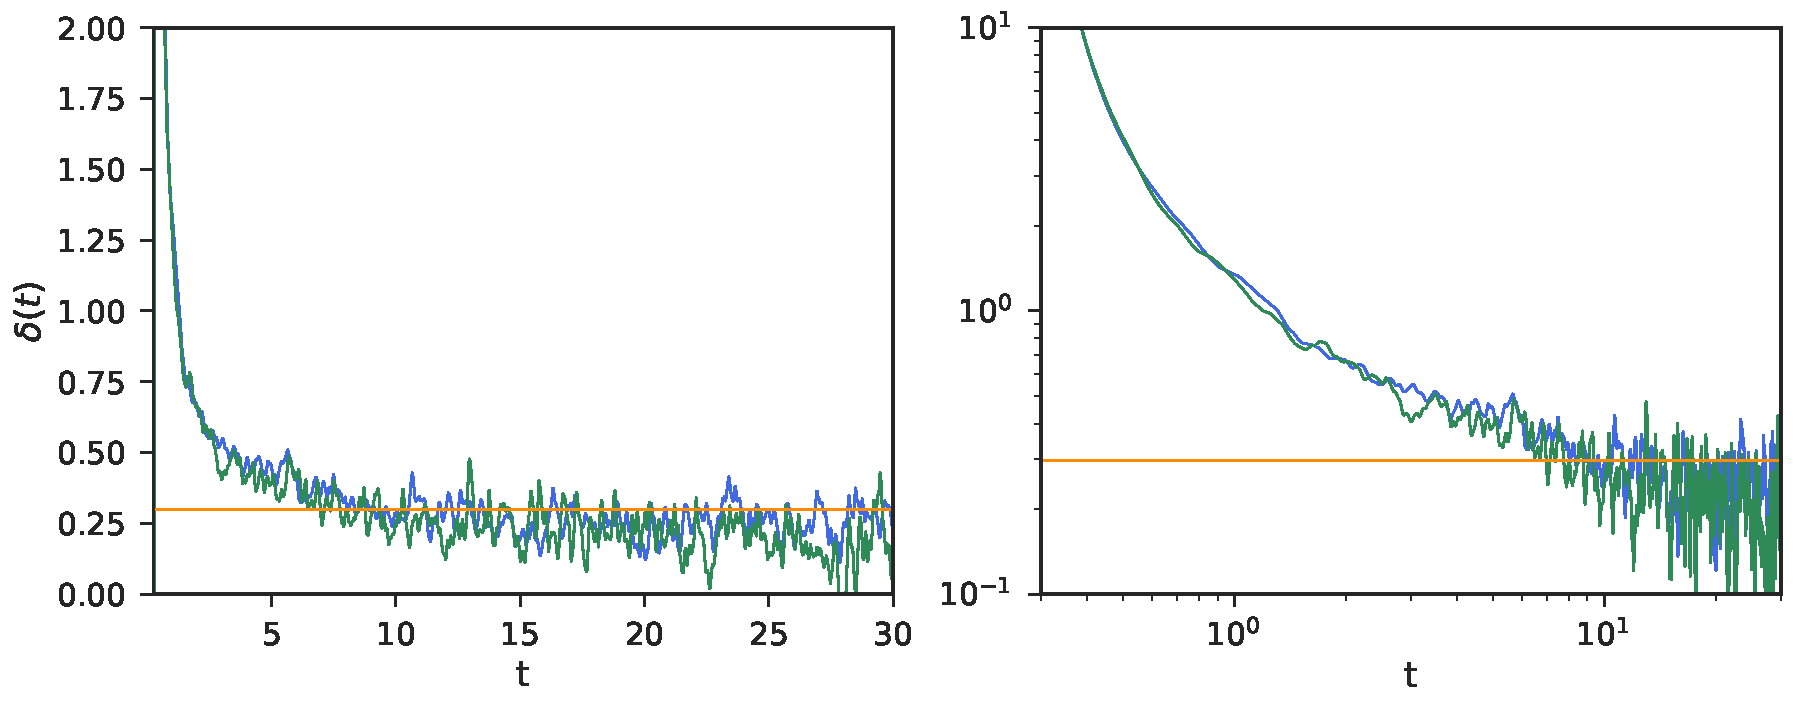
\includegraphics[width=\linewidth]{Slipt-17nodes-WALLS}
  \end{figure}
  \begin{itemize}
    \item The slip length does not depend on the channel width (left) and is roughly independent of the actual value of $\tau$ (right).
  \end{itemize}
\end{frame}

\begin{frame}{Local hydrodynamic model with boundary conditions}  
  \begin{itemize}
    \item The disrete version of the local equation $\partial_t g(z,t)=\nu\frac{\partial^2}{\partial z^2} g(z,t)$
\begin{align}
  \frac{d}{dt}g_\mu(t)&=\nu \frac{1}{\Delta z^2}(g_{\mu-1}(t)+g_{\mu+1}(t)-2g_{\mu}(t))
\nonumber
\end{align}
where the kinematic viscosity is $\nu=\frac{\eta}{\rho}$.
    \item Nonlocal hydrodynamic equation  
\begin{align}
  \frac{d}{dt}{\bf g}^x_\mu(t)=&
-\sum_{\nu} {\cal V}_\nu \frac{\left[\eta_{\mu\nu}-\eta_{\mu-1\nu}-\eta_{\mu\nu-1}+\eta_{\mu-1\nu-1}\right]}{\Delta z^2}\overline{\bf v}^x_\nu \nonumber \\
  &{\color{red}+\sum_{\nu} {\cal V}_\nu\frac{\left[G_{\mu\nu}-G_{\mu\nu-1}\right]}{\Delta z}\overline{\bf v}^x_\nu
+\sum_{\nu} {\cal V}_\nu\frac{\left[H_{\mu\nu}-H_{\mu-1\nu}\right]}{\Delta z}
  \overline{\bf v}^x_\nu}
\nonumber \\
  &{\color{red}-\sum_{\nu} {\cal V}_\nu\gamma_{\mu\nu}\overline{\bf v}^x_\nu}
\nonumber
\end{align}
\item We use the slip boundary condition $\overline{\bf v}_{\rm wall}^x=\delta \dot{\overline{\gamma}}_{\rm wall}$ applied at $z_{\rm wall}$.
  \end{itemize}
\end{frame}

\begin{frame}{The local predictions}
\begin{align}
 g(t)&=\exp\{\nu \Delta' (t-\tau)\}g(\tau)
\nonumber
\end{align}
%with $\Delta'$ the Laplacian operator for slip boundary condition.
\begin{figure}[]
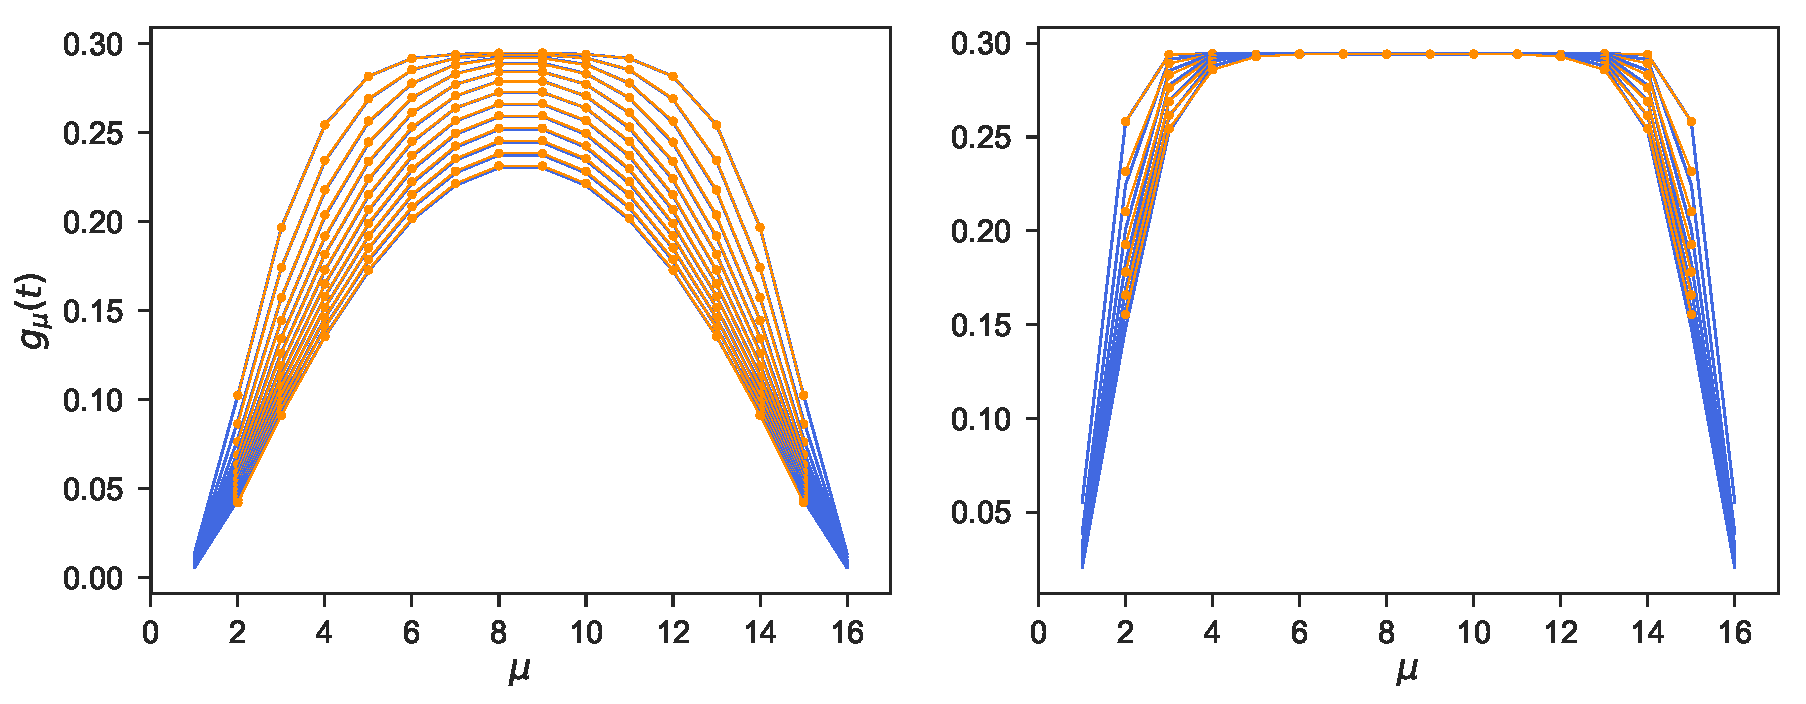
\includegraphics[width=\linewidth]{gxtLocalPrediction-17nodes-WALLS}
\end{figure}
  {\color{orange} Local  prediction}
  compared with the {\color{blue} measured} momentum density
  profile. Times  are $t=5,7,\cdots,29$  (left panel) in descending  order. Times $t=0.3,0.6,\cdots2.1$ (right panel).
\end{frame}

\begin{frame}{Comparison of the error between local and nonlocal theories}
  \begin{align}
  err_\mu(t)=  g_\mu(t)-g^{\rm predict}_\mu(t)
    \nonumber
  \end{align}
    \begin{figure}
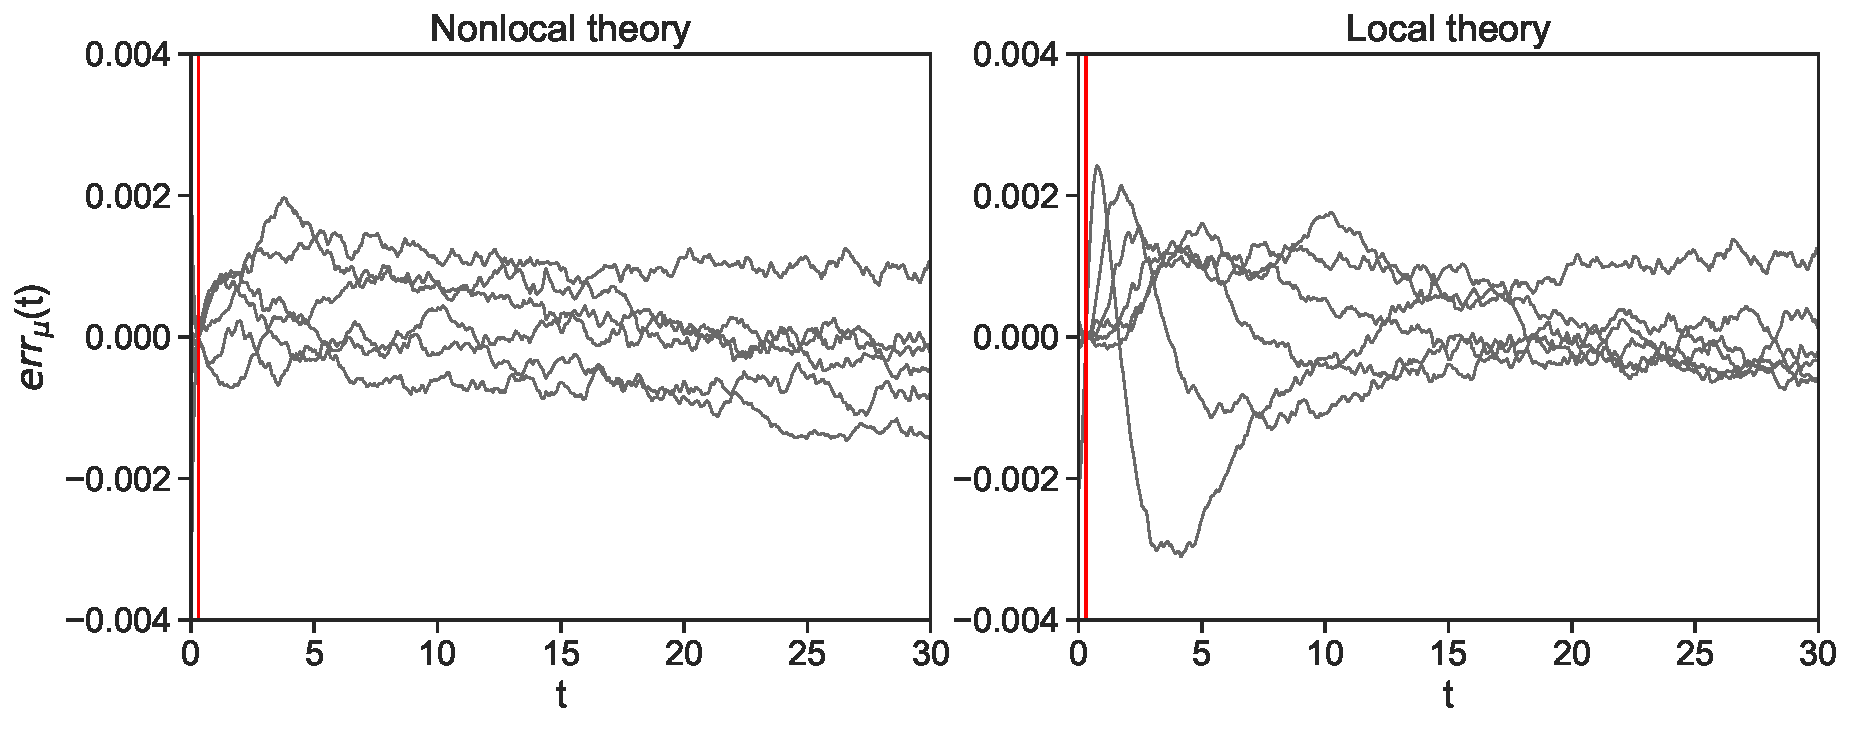
\includegraphics[width=\linewidth]{errors-17nodes-WALLS-defense}
\end{figure}
  %\begin{itemize}
    %\item The local theory gives higher errors. 
    %\item The slip boundary condition used to predict the flow does not hold. 
    %\item It is necessary to consider the explicit interaction between the solid and the fluid through the surface irreversible forces containing the transport kernels $G_{\mu\nu}$,$H_{\mu\nu}$,$\gamma_{\mu\nu}$.
    %\item While the local prediction with the slip boundary condition is acceptable, nonlocal effects are appreciable. 
  %\end{itemize}
\end{frame}

\begin{frame}{Conclusions}

\end{frame}

\begin{frame}{Future Directions}
  \begin{enumerate}
        \item Non-Markovian effects may be related to the ``hard'' nature of the crystal. 
      \begin{itemize}
        \item More realistic models for the solid wall. 
        \item Change the thermodynamic point. 
        \item Hydrofobicity or hydrofillicity affect the conclusions. 
      \end{itemize}
    \item Non-isothermal theory. 
      \begin{itemize}
        \item New CG variables
\begin{align}
  \hat{e}_{\bf r}(z) = \sum_i^N e_i\delta({\bf r}-{\bf q}_i) &&  \hat{E}(z)=\sum_{i'}^{N'}e_{i'}
  \nonumber
\end{align}
\item Solve the problem of thermal boundary conditions. 
    \item Understand the heat transfer between solids and fluid, specifically between nanoparticles and molten salts. 
      \end{itemize}
  \end{enumerate}
\end{frame}

\begin{frame}{Relevant references}
  \begin{itemize}
      \begin{small}
    \item D.Camargo, J.A. de la Torre, {\bf D.Duque-Zumajo}, P.Espa\~nol, R.Delgado-Buscalioni, and F. Chejne. Nanoscale hydrodynamics near solids. \textit{Journal of Chemical Physics}, 148(6), 2018.
    \item P.Espa\~nol, J.A.de la Torre, and {\bf D.Duque-Zumajo}. Solution to the plateau problem in the Green-Kubo formula. \textit{Physical Review E}, 99(2), 2019.
    \item {\bf D. Duque-Zumajo}, D. Camargo, J. A. de la Torre, F. Chejne, and Pep Espa\~nol. Discrete hydrodynamics for planar flows with confining walls. \textit{Physical Review E}, 2019.
  \item {\bf D. Duque-Zumajo}, J. A. de la Torre, and Pep Espa\~nol. Slip and non-Markovian effects in nanohydrodynamics (in preparation). \textit{Physical Review Letters}, 2019. 
  \item {\bf D. Duque-Zumajo}, D. Camargo, J. A. de la Torre, Farid Chejne, and Pep Espa\~nol. Discrete hydrodynamics near solid walls: non-Markovian effects and slip (in preparation). \textit{Physical Review E}, 2019. 
      \end{small}
  \end{itemize}
\end{frame}

\begin{frame}
\begin{figure}

\includegraphics[width=0.2\linewidth]{logo}
\end{figure}
  \vspace{0.5cm}  
\begin{center}
\textit{Nanoscale hydrodynamics near solids}\\
July 2019\\
Diego Duque Zumajo
\end{center}

\end{frame}

\begin{frame}{Dual basis functions and mass matrix}
  \begin{itemize}
  \item We can contruct continuum and discrete fields from dual basis functions $\delta_{\mu}({\bf r})$ and $\psi_\mu({\bf r})$ 
    \begin{align}
      v_\mu=\int d{\bf r}v({\bf r})\delta_\mu({\bf r}),&&
        \overline{v}({\bf r}) =\sum_{\mu}v_\mu\psi_\mu({\bf r})
    \nonumber
    \end{align}
    \item The usual mass matrix of the finite element method is
      \begin{align}
      M^\Phi_{\mu\nu}&=\llg\Phi_\mu\Phi_\nu\rlg  
      \nonumber
      \end{align}
      where we have introduce the notation $\llg\cdots\rlg=\int d{\bf r}...$
    \item We introduce the discrete velocity field in terms of $M^\Phi_{\mu\nu}$
      \begin{align}
        \tilde{{\bf v}}_{\mu}=\sum_{\nu}{\cal V}_{\mu}[M^{\Phi}]^{-1}_{\mu\nu}{\bf v}_{\nu}
        \nonumber
      \end{align}
  \end{itemize}
\end{frame}

\begin{frame}{Normal and tangent evolution}
\begin{itemize}
  \item The normal evolution 
\begin{align}
  \frac{d}{dt}\rho_\mu=&  {\color{blue} \llg\overline{\rho} \; \overline{v}^{z}{\nabla}^{z}\delta_\mu \rlg}
\nonumber\\
    \frac{d}{dt}{{\bf g}}^{z}_\mu=&
{\color{blue} \llg\overline{\rho}\; \overline{v}^{z}\;\overline{v}^{z}{\nabla}^{z}\delta_{\mu}\rlg
-\llg\overline{\rho}\delta_{\mu}{\nabla}^{z}\delta_{\nu}\rlg
\frac{\partial  F}{\partial \rho_{\nu}}(\rho)}
{\color{red} +M_{\mu\nu}^{\bot}{\cal V}_\nu\tilde{v}^{z}_\nu}
\nonumber
\end{align}
  \item The parallel evolution for $\alpha=x,y$  
\begin{align}
  \frac{d}{dt}{{\bf g}}^\alpha_\mu=&{\color{red}-M_{\mu\nu}^{||}{\cal V}_\nu\tilde{v}^\alpha_\nu}
\nonumber
\end{align}
\item The dissipative matrix for $\odot=||,\bot$
\begin{align}
M^{\odot}_{\mu\nu} 
=&-\frac{\eta^{\odot}_{\mu\nu}-\eta^{\odot}_{\mu-1\nu}-\eta^{\odot}_{\mu\nu-1}+\eta^{\odot}_{\mu-1\nu-1}}{\Delta z^2}
+\frac{{G}^{\odot}_{\mu\nu}-{G}^{\odot}_{\mu\nu-1}}{\Delta z} \nonumber \\
&+\frac{{H}^{\odot}_{\mu\nu}-{H}^{\odot}_{\mu-1\nu}}{\Delta z}
-{\gamma}^{\odot}_{\mu\nu}
\nonumber
\end{align}
\end{itemize}
\end{frame}

\begin{frame}{Mori's theory}
  \begin{itemize}
    \item<1-> Linear dynamic equations not only for the averages of the relevant variables but also for their correlations
\begin{align}
  \frac{d}{dt}C(t)&=-L\esc C^{-1}(0)\esc C(t)
  -{\color{red}\int_0^tdt' \Gamma(t-t')\esc C^{-1}(0)\esc  C(t')}
\nonumber
\end{align}
where the following matrices have been introduced
\begin{align}
  L&=\langle \hat{A}i{\cal L}\hat{A}^T\rangle \nonumber \\
  C(0)&=\langle \hat{A}\hat{A}^T\rangle \nonumber \\
\Gamma(t)&=\langle F^+(t)F^{+T}(0)\rangle
\nonumber
\end{align}
\item<2-> The projected forces are given by
\begin{align}
F^+(t)&= \exp\{{\cal Q}i{\cal L}t\} {\cal Q}i{\cal L}\hat{A}  
\nonumber
\end{align}
\item<3-> ${\cal Q}=1-{\cal P}$ where  ${\cal P}$  is Mori's  projector 
\begin{align}
  {\cal P}\hat{F}(z) = \langle \hat{F}\rangle+ \langle \hat{F}\hat{A}^T \rangle\esc  C^{-1}(0)\esc  \hat{A}(z)
\nonumber
\end{align}
\end{itemize}
\end{frame}

\begin{frame}{Markovian approximation}
  \begin{itemize}
    \item Memory-less term 
  \begin{align}
{\color{red}\int_0^tdt' \Gamma(t-t')\esc C^{-1}(0)\esc  C(t')} \simeq M^* C^{-1}(0)C(t)
\nonumber
\end{align}
\item Expression for the correlations
\begin{align}
  \frac{d}{dt}C(t) &= - (L+M^*)\esc C^{-1}(0)\esc C(t) \nonumber \\
                     &\equiv \Lambda^*\esc C(t)
  \nonumber
\end{align}
\item For a linear Markovian theory the only possibility for a correlation is to decay in an exponential matrix way
\begin{align}
  C(t)=\exp\{-\Lambda^* (t-\tau)\}\esc C(\tau)
\nonumber
\end{align}
\item {\bf We need to find a constant matrix $\boldsymbol{\Lambda^*}$}.
\end{itemize}
\end{frame}

\end{document}
